%
% This text file include all filess neccessary to create
% the User's Guide
%

%====== define a new class for layout

\documentclass[a4paper]{../covise}

\usepackage{makeidx}
\makeindex

%====== set some useful packages for HTML, color, graphics, longer table
%====== floating text around images , pdf-links ...

\usepackage{html, htmllist}
\usepackage{hyperref}
\usepackage{color}
\usepackage{graphicx}
\usepackage{longtable}
\usepackage{codoxygen}

%\usepackage{mathpazo}
%\usepackage{newcent}
\usepackage{pslatex}
%\renewcommand{\familydefault}{\sfdefault}

\usepackage[T1]{fontenc}
%\renewcommand{\sfdefault}{uop}

\newcommand{\code}[1]{{\sffamily #1}}
\newcommand{\arrow}{-\textgreater}

\setlength\LTleft{0pt}
\setlength\LTright\fill

%====== start the document

\begin{document}


%====== the following tables are only used by PS/PDF
%====== also the titlepage and the next page
\begin{latexonly}

\begin{titlepage}
    \setcounter{page}{0}
	 \thispagestyle{empty}
    \unitlength1cm
    
       \begin{picture}(15,17)
       \put(2, -2.5){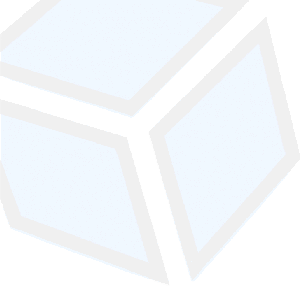
\includegraphics[scale=5]{../visenso_title}}     
       \put(0,-3){\line(1,0){15}}
       \put(0, 10){\makebox(15,2)[t]{\Huge{COVISE}}}
       \put(0, 9){\makebox(15,2)[t]{\Huge{Programming Guide}}}          
       \end{picture}
    
	\newpage
   \setcounter{page}{0}
	\thispagestyle{empty}
   \uppertitleback{\bf{Title:} \\
			COVISE Programming Guide \\
         \today }
   \vfill
	\lowertitleback{\bf{Authors:} \\
         Martin Aum\"uller \\
         Andreas Werner \\
         Uwe Woessner }

\end{titlepage}

	\pagenumbering{arabic}
	\tableofcontents
%	\listoffigures
%	\listoftables
	
\end{latexonly}


%====== include the chapters


\begin{htmlonly}

\usepackage{html, htmllist}
\usepackage{longtable}

\bodytext{bgcolor="#ffffff" link="#0033cc" vlink="#0033cc"}

%%%==================================================	
%%%==================================================	

% #1  mark defined by \label
% #2  a linktext 
% #3  a html link 
\newcommand{covlink}[3]{\htmladdnormallink{#2}{#3} \latex{(\ref{#1})} }


\newenvironment{covimg}[4]%
{
 \begin{figure}[htp]
  \begin{center}
   \latexonly
      \includegraphics[scale=#4]{#1/pict/#2}
   \endlatexonly  
   \html{\htmladdimg[align="center"]{pict/#2.png}}
   \caption{#3}
  \end{center}
 \end{figure} 
}{} 

\newenvironment{covimg2}[3]%
{ 
 \begin{figure}[htp]
  \begin{center}
     \latexonly
       \includegraphics[scale=#3]{#1/pict/#2}   
     \endlatexonly
     \html{\htmladdimg[align="center"]{pict/#2.png}}
  \end{center}
 \end{figure} 
}{}

\definecolor{output}{rgb}{0.,0.,1.}
\definecolor{depend}{rgb}{1.,0.65,0.}
\definecolor{required}{rgb}{0.58,0.,0.83}
\definecolor{optional}{rgb}{0.,0.39,0.}

\newcommand{\addimage}[1] {\html{\htmladdimg{pict/#1.png}}}

\newcommand{\addpict}[4] {\latexonly
	     \begin{figure}[!htbp]
			  \begin{center}
   	 		  \includegraphics[scale=#1]{#2}
   	 		  \caption{#3}
		 		  \label{#4}
			  \end{center}
	 		\end{figure}
	     \endlatexonly}



\end{htmlonly}



%=============================================================
\startdocument
\chapter{Basics}
\label{Basics}
%=============================================================
\index{Basics}


\section{Introduction}

This documentation describes how to integrate new application modules into COVISE.
There is also a section describing how to write plugins for the VR renderer.
The programming functionality to interface and communicate with COVISE is explained 
in detail.

Currently, each COVISE module is realized as an operating system process.
Future versions may allow to create modules which are modeled as subroutines or
threads in a single process environment.

\section{Prerequisites}
\latexonly
\index{Prerequisites}
\endlatexonly

To create new COVISE modules, the COVISE development distribution with all the 
necessary header files and libraries has to be installed on the target platform. 
For UNIX and similar systems, this includes also a set of scripts for Bourne
Shell compatible shells
to set up your compile environment, especially the environment variables necessary
for compiling COVISE.
Start a bash by typing \texttt{bash} (if this is not your default shell), change to the
COVISE top level directory and type \texttt{source .covise.sh}.
If your current working directory is not the COVISE top level directory
and if your home directory does not contain the covise top level directory then you have to pass the
location of this directory as a parameter to this script.

When compiling modules, COVISE automatically creates different directories for 
platform-specific parts like object files and executables: object files are generated 
in the objects\_\$ARCHSUFFIX subdirectory of your source directory, while binaries are put in 
\$COVISEDIR/\$ARCHSUFFIX/bin, where \$ARCHSUFFIX is a platform identifier. Refer to
\$COVISEDIR/README-ARCHSUFFIX.txt for a full list. Here are some examples:

\begin{longtable}{|p{2.5cm}|p{12cm}|}
\hline
   {\bf ARCH} & {\bf Platform}  \endhead
\hline\hline
   rhel6 & RedHat Enterprise Linux 6.x or compatible (CentOS, Scientific Linux) \\
\hline
	win32 &  Microsoft Windows using the Visual Studio 2003 compiler \\
\hline
	lion &  Apple Mac OS X 10.7 (x86\_64)\\
\hline
\end{longtable}
{\bf Table 1: Architecture suffixes}
\index{Architecture suffix}

There are following requirements before starting to program:

\begin{itemize}

   \item A \texttt{CMakeLists.txt} file \index{CMake} used by CMake to generate a Makefile \index{Makefile} or
compile instructions for other build environments: examples are available with the example modules, 
which reside in \verb+$COVISEDIR/src/application/Examples+.
You can also use the template in \verb+$COVISEDIR/src/template/module+ as a
starting point.

\item A directory for the source code of the module is required.

\item The {\tt Hello} module in {\tt \$COVISEDIR/src/application/Examples/Hello} defines 
the complete basic structure of a module. It is recommended to copy this module source 
code as the base for own developments.

\end{itemize}

For users of the make build system having sourced the .covise.sh setup file,
compiling the module is as simple as typing \texttt{make} in the module source directory.

COVISE has an object-oriented architecture requiring static initialization of 
multiple classes. For proper initialization, the main body of each module has to be 
written in C++. Nevertheless it is possible to integrate FORTRAN and C routines into 
an application module. 

Each module is executed as a separate operating system process.
Modules communicate in general 
using TCP/IP socket connections.
This applies within a machine as well as between 
machines.
Data exchange is handled differently. Within a machine pointers to shared 
memory are used  to avoid copying of data objects. Between machines data objects are 
exchanged via TCP/IP socket connections. All this is handled transparently  for  
the application programmer.
The COVISE API (Application Programming Interface) is 
accessible through several libraries, which have to be linked to each new module. 
This happens automatically, if you specify \texttt{covise\_add\_module} as done
in the CMakeLists.txt for the module template.
\index{cmake!template}

The main COVISE library is called {\tt libcoCore.so}
({\tt .sl} on HP, \texttt{.dll}/\texttt{.lib} on Windows, \texttt{.dylib} on Mac OS X).
It is used for data management, message communication, starting processes, etc.
\index{Libraries!coCore}

The Application library, called {\tt libcoAppl.so}, contains the basic functionality to 
write application programs. It hides the details of packing and receiving COVISE 
messages and provides a framework for structuring application modules.
\index{Libraries!coAppl}

The library {\tt libcoApi.so} builds on these libraries and provides the
Application Programming Interface, which makes programming of applications
easier and less error-prone.
Whenever possible, programmers are recommended to use the higher level API
functions instead of the direct COVISE calls provided with the Application library.
\index{Libraries!coApi}

\section{Data flow model}
\latexonly
\index{Data flow}
\endlatexonly

COVISE sessions are organized as a collection of modules, which are connected in a 
strictly unidirectional data flow network.

A typical data flow network is shown in the next figure.  Data and control flows from top to 
bottom. Loops are not allowed, nevertheless, there are possibilities to send feedback 
messages from later to earlier modules in the processing chain.

\begin{covimg}{Basics}{Module_and_Dataflow_network}{Module and Dataflow network}{0.7}\
\end{covimg}
\begin{htmlonly}
Figure: Module and Dataflow network
\vspace*{1cm}
\end{htmlonly}

Each module in the pipeline communicates with the central controller
(the process named \texttt{covise}) and a local 
data-manager (named \texttt{crb}) by sending or receiving control messages via a TCP/IP socket. 
Data flow between modules is only a visual metaphor. Within a machine data objects are 
stored in shared memory segments. They are accessible from different modules by mapping
their storage into the address space of the respective module processes. Between 
machines, objects are transferred by COVISE request brokers (CRBs), including necessary 
format conversions. This is transparent for the modules accessing the data objects. 
Both data and control communication are completely hidden within the
COVISE libraries.

\section{Execution sequence and module states}
\latexonly
\index{Execution sequence} 
\index{module states}
\endlatexonly

The sequence of states a COVISE module can have is shown in the following figure.

\begin{covimg}{Basics}{Module_execution_scheme}{Module execution scheme}{0.7}\
\end{covimg}
\begin{htmlonly}
Figure: Module execution scheme
\vspace*{1cm}
\end{htmlonly}

The start-up of a module \index{coModule!start-up} is divided into two parts: The Constructor creates the module 
layout, which is sent to the COVISE controller using the module start message.
In order to avoid timeout conditions during running the constructor,
time consuming initialization operations should be put into an additional user subroutine
which is called after establishing the COVISE connectivity to allow user-supplied start-up routines to 
be performed without timeout problems. After the start-up sequence, COVISE enters a 
main event loop, which is only left for the module shut-down. In the main loop, COVISE 
can receive different events, which are then handled by one of the following event 
handlers:

\begin{itemize}

\item {\it param}: Every change of a module parameter submits a message 
to the module. The \texttt{param} subroutine reacts on these change messages.

\item {\it compute}: COVISE tells the module to read its input data and create output data. 
Only within this routine data objects in shared memory can be read or new data objects 
in shared memory can be created.

\item {\it sockData}: The user can register open network sockets to be monitored. Whenever 
data on one of these sockets arrives, sockData is called.

\end{itemize}

It is important to note that several commands are only allowed when COVISE is in the 
appropriate state. Due to performance reasons these states are not generally checked, 
thus calling functions during illegal states may result in module crashes.



\begin{htmlonly}

\usepackage{html, htmllist}
\usepackage{longtable}

\bodytext{bgcolor="#ffffff" link="#0033cc" vlink="#0033cc"}

%%%==================================================	
%%%==================================================	

% #1  mark defined by \label
% #2  a linktext 
% #3  a html link 
\newcommand{covlink}[3]{\htmladdnormallink{#2}{#3} \latex{(\ref{#1})} }


\newenvironment{covimg}[4]%
{
 \begin{figure}[htp]
  \begin{center}
   \latexonly
      \includegraphics[scale=#4]{#1/pict/#2}
   \endlatexonly  
   \html{\htmladdimg[align="center"]{pict/#2.png}}
   \caption{#3}
  \end{center}
 \end{figure} 
}{} 

\newenvironment{covimg2}[3]%
{ 
 \begin{figure}[htp]
  \begin{center}
     \latexonly
       \includegraphics[scale=#3]{#1/pict/#2}   
     \endlatexonly
     \html{\htmladdimg[align="center"]{pict/#2.png}}
  \end{center}
 \end{figure} 
}{}

\definecolor{output}{rgb}{0.,0.,1.}
\definecolor{depend}{rgb}{1.,0.65,0.}
\definecolor{required}{rgb}{0.58,0.,0.83}
\definecolor{optional}{rgb}{0.,0.39,0.}

\newcommand{\addimage}[1] {\html{\htmladdimg{pict/#1.png}}}

\newcommand{\addpict}[4] {\latexonly
	     \begin{figure}[!htbp]
			  \begin{center}
   	 		  \includegraphics[scale=#1]{#2}
   	 		  \caption{#3}
		 		  \label{#4}
			  \end{center}
	 		\end{figure}
	     \endlatexonly}



\end{htmlonly}


%=============================================================
\startdocument
\chapter{Module Programming}
\label{Module Programming}
%=============================================================
\index{coModule}


\section{The \code{coModule} Base Class}

The base class for all module programming is {\tt coModule}. An application is created 
by deriving a class of {\tt coModule}. The constructor of the derived class creates 
the module layout with input ports, output ports and parameters. Virtual functions are 
overloaded to implement the module's reactions on events.  Every COVISE
module based on {\tt coModule} looks like:

\underline{Header file:}
\begin{verbatim}
class myMod: public coModule
{
   private:
      ... // parameter and data object ports

   public:
      myMod(int argc, char *argv[]);     // Constructor: module set-up
      virtual void compute(const char *);       // Called for every execute
      virtual void param(const char *, bool inMapLoading);
                                         // Called for param changes
      virtual void sockData(int sockNo); // Called for receiving data
}
\end{verbatim}

\underline{Source code:}
\begin{verbatim}
myMod::myMod(int argc, char *argv[])
: coModule(argc, argv, "My example module")
                               {...}    // build ports and parameters
myMod::compute(const char *)         {...}    // module is executed
myMod::param(const char *, bool inMapLoading)
                               {...}    // parameters changed
myMod::postInst(const char *)  {...}    // between c'tor and main loop
myMod::quit(const char *)      {...}    // after the end of main loop
myMod::sockData(int socNo)     {...}    // data arrived on a socket

MODULE_MAIN(SomeCategory, myMod)

\end{verbatim}

To allow future use of threads and multi-linked modules, modules should use neither global nor non-constant
static variables.

\section{\code{coModule}'s Functions}

{\Large Constructor}
\index{coModule!constructor}
\vspace*{0.5cm}

The constructor of a module is used to set up its external connectivity. First, it calls the constructor of the base
class {\tt coModule}:

\begin{verbatim}
      void coModule::coModule(int argc, char *argv[], const char *description=NULL, bool propagate=false)
\end{verbatim}

The constructor of \code{coModule} establishes some basic data structures and pre-sets 
them with defaults values.

The execution of a module constructor is time-critical. If the constructor is not finished within the timeout period
given in the config file, the CRB will not accept the module and the user interface will issue an error message
telling that the module did not start. 

In general, the constructor should never do anything else than defining the 
ports and parameters of the module.

\vspace*{1cm}
{\Large postInst}
\index{coModule!postInst}
\vspace*{0.5cm}

For any additional functionality required before entering the main loop the routine 

\begin{verbatim}
      virtual void coModule::postInst()
\end{verbatim}

should be overloaded by the module. It is called once before entering the main event loop. This avoids timeouts,
which could occur as described in the constructor paragraph.

\vspace*{1cm}
{\Large param}
\index{coModule!param}
\vspace*{0.5cm}

Since COVISE 6.1, a module is notified immediately unconditionally when a parameter was
changed by the user (i.~e. all parameters are ``immediate'' now).
For any changed  parameters, the callback

\begin{verbatim}
      virtual void coModule::param(const char *paramName, bool inMapLoading)
\end{verbatim}

is called with the name of the port as the parameter.

\vspace*{1cm}
{\Large compute}
\index{coModule!compute}
\vspace*{0.5cm}

The compute callback is called whenever new input data for a module is available or when the user executes a
module manually.
 
\begin{verbatim}
      virtual int coModule::compute(const char *)
\end{verbatim}

Before calling the user supplied routine,
the input objects are retrieved from the data manager and the object pointer is stored 
to be retrieved from the port. The return value of the compute callback must be either 
CONTINUE\_PIPELINE or STOP\_PIPELINE depending on whether modules below should be 
executed or not.

Most modules only need a compute function and do not use the other functions. All 
functions are pre-initialized with empty functions in case the user does not overload 
them. A warning is submitted if compute(const char *) is executed without being overloaded.

\vspace*{1cm}
{\Large sockData}
\index{coModule!sockData}
\vspace*{0.5cm}

If a module needs to use any other external communication means than the COVISE internal
networking, e.~g.\ connect to a simulation or use the X Window system, the programmer has to make 
sure that COVISE messages are still received and handled. Therefore, a file descriptor, 
e.~g.\ a socket, can be registered with the module via

\begin{verbatim}
      void addSocket(int fd)
\end{verbatim}

Once this has been done, COVISE adds the socket to its own sockets and calls the 
virtual function

\begin{verbatim}
      virtual void coModule::sockData(int fd)
\end{verbatim}

with the file descriptor as the argument. The user can then handle the input and return 
control to COVISE by leaving the callback. After use, the socket is removed using

\begin{verbatim}
      void removeSocket(int fd)
\end{verbatim}

\vspace*{1cm}
{\Large quit}
\vspace*{0.5cm}

A module terminates either when COVISE terminates, the user deletes a module or a new 
map is loaded. To allow cleaning up resources, the routine

\begin{verbatim}
      virtual void coModule::quit()
\end{verbatim}

is automatically called before the module quits.

\vspace*{1cm}
{\Large idle}
\vspace*{0.5cm}

The idle function is called whenever the module waits for COVISE messages.

\begin{verbatim}
      virtual float coModule::idle()
\end{verbatim}

You should not block in this function, otherwise the module will never get the chance to
process incomming messages. If you overwrite this method, you have to return a float 
value. This value specifies the maximum number of seconds to wait until the idle function
is called again. If zero is returned, the idle function is called again immediately after
checking for COVISE messages. If a negative value is returned, the idle function will 
not be called until any message arrived. If  a positive Value is returned, the idle 
function will be called after the appropriate time, or earlier if any message arrived.

Remember: You can't create COVISE distributed objects in this callback! 

\vspace*{1cm}
{\Large Other coModule functions}
\vspace*{0.5cm}

\begin{verbatim}
      virtual void feedback(int len, const char *data);
\end{verbatim}

This function is called when a COVER plugin sends a feedback message.

\begin{verbatim}
      virtual void feedbacksetInfo(int len, const char *datatext);
\end{verbatim}

Allows to set an info string in the control panel of the module.

\section{coSimpleModule Set-Handler}

COVISE can handle hierarchical structures of data created by Set containers, e.g. 
timestep series or data sets consisting of multiple distinct parts. A module handling 
these data types has to be written recursively to be able to handle arbtrary levels 
of hierarchy. In most cases, modules work with `corresponding' data, e.g. a set of 
geometry objects required an identical set of colors and normals, or a set of timesteps of a moving grid simulation
corresponds to a similar set of data values. 

For easier module development, the class \code{coSimpleModule} has been derived from 
coModule. It automatically un-packs all level of Set containers until reaching 
the lowes level, and then calls compute(const char *) for each low-level object. The module 
developer simply creates the module and writes a compute(const char *) function as if the data was 
non-hierarchical, which is then called for every corresponding set of low-level object. 

The functions

\begin{verbatim}
      void setComputeTimesteps(const int off);    // 0 by default
      void setComputeMultiblock(const int off);   // 0 by default
\end{verbatim}

can be called if the user wants to handle timesteps or multiblock data  himself, 
e.g. for particle tracing. 

The simple module also automatically copies all attributes from the input objects to the output objects at the port directly underneath the input port. If
this is not desired, it can be switched of by calling

\begin{verbatim}
      void setCopyAttributes(const int on);      // 1 by default
\end{verbatim}


\section{Ports and Parameters}
%\index{Ports}
%\index{Parameters}

Ports establish the connection of a module to the rest of the COVISE system. Three 
different kinds of connections can be defined:

\begin{enumerate}
\item Parameters:        Values interactively set in the Map-Editor by the user 
\item Input data ports:  Receive data from other modules
\item Output data ports: Send data to other modules
\end{enumerate}

All ports and parameters are created by calling a member function of \code{coModule}
that returns a pointer to a port class object, which can later be used to set or 
retrieve port data. These pointers will usually be stored as module
class private data being usable in the whole module. 

The creation of ports and parameters only possible in the Constructor state, a later 
creation of ports is not supported. Ports can be hidden or de-activated if not currently
needed.

\vspace*{0.5cm}

\textbf{Never create Modules with variable numbers of Ports or Parameters: 
These modules will crash COVISE when being read from a map file!}

\vspace*{0.5cm}

%\begin{covimgpath}{ModuleProgramming}{Warning1}{0.8} \end{covimg2}

All ports and parameters must have a unique name and description, which can be any text 
explaining the function of the port. Names must not contain blank characters or any 
special ASCII characters like TAB, CR, LF, DEL, BS. The description may contain blanks, 
but no special characters like CR, LF or BS characters and need not be unique.

Never construct a port or parameter by its own constructor, COVISE must register it with 
the module. Instead, the functions \code{add<type>Port} and \code{add<type>Param} have 
to be used.

All input and parameter ports derive from the same base class coUifElem, which implements
some base functionality for all kinds of ports. The following subroutines can therefore 
be called for all parameter and port class objects: 
\index{Ports!common functions}
\index{Parameters!common functions}

\begin{longtable}{|p{4cm}|p{10cm}|}
\hline
\multicolumn{2}{|p{13.5cm}|}{\bf const char *coUifElem::getName() const} \\
\hline
{Description:}   & {Get port's name} \\
\hline
{COVISE states:} & {all} \\
\hline
{Return value:}  & {Port name} \endhead
\hline
\end{longtable}
\index{coUifElem!getName}

\begin{longtable}{|p{4cm}|p{10cm}|}
\hline
\multicolumn{2}{|p{13.5cm}|}{\bf const char *coUifElem::getDesc() const} \\
\hline
{Description:}   & {Get port's description} \\
\hline
{COVISE states:} & {all} \\
\hline
{Return value:}  & {Port description} \endhead
\hline
\end{longtable}
\index{coUifElem!getDesc}

\begin{longtable}{|p{4cm}|p{2.5cm}|p{7cm}|}
\hline
\multicolumn{3}{|p{13.5cm}|}{\bf virtual void coUifElem::print(ostream \&str) const} \endhead
\hline
{Description:}   & 
                       \multicolumn{2}{|p{9.5cm}|}{Print port information into a stream} \\
\hline
{COVISE states:} & \multicolumn{2}{|p{9.5cm}|}{all} \\
\hline
\multicolumn{1}{|r|}{IN:}  & {str} & 
                                  {stream to print into} \\
\hline
\end{longtable}
\index{coUifElem!print}


\section{Data Ports}

When replacing modules, data port connections can only be maintained if the ports adhere to a
common naming scheme.
A port name should start with a prefix from the following table.
If the port is able to accept data types from several lines in this table, then choose ``Data'',
except for when it is Geometry and grid types, then choose ``Grid''.
As appropriate, append ``In'' or ``Out'' to the prefix.
Finally you should append the number of the port: start with ``0'' for the first port with a
certain prefix and direction, and increase the number for each other port with the same prefix
and direction.
Also append the final ``0'' if there is only one port of this type.


\begin{longtable}{|p{4cm}|p{9.5cm}|}
\hline
{Name prefix} & {Data object types} \\
\hline\hline
Data & Int, Float, Vec2, Vec3, RGBA, Mat, Tensor \\
\hline
Grid & Points, Spheres, Lines, Polygons, TriangleStrips,
     
     UniformGrid, RectilinearGrid, StructuredGrid, UnstructuredGrid \\
\hline
Geometry & Geometry \\
\hline
Texture & Texture \\
\hline
\end{longtable}

Data ports are created by:

%\begin{longtable}{|p{4cm}|p{2.5cm}|p{7cm}|}
%\hline
%\multicolumn{3}{|p{13.5cm}|}{\bf coInputPort *coModule::addInputPort(const char *name,const char *typeList, 
%const char *desc)} \\
%\hline
%{Description:}   & 
%                       \multicolumn{2}{|p{9.5cm}|}{Create an Input data port} \\
%\hline
%{COVISE states:} & \multicolumn{2}{|p{9.5cm}|}{Constructor} \\
%\hline
%\multicolumn{1}{|r|}{IN:}  & {name:} & 
%                                  {Port name} \\
%\hline
%\multicolumn{1}{|r|}{IN:}  & {typeList:} & 
%                                  {Map editor data types} \\
%\hline
%\multicolumn{1}{|r|}{IN:}  & {desc:} & 
%                                  {Parameter description} \\
%\hline
%{Return Value:}   & 
%                       \multicolumn{2}{|p{9.5cm}|}{pointer to newly created port} \endhead
%\hline
%\end{longtable}


\begin{longtable}{|p{4cm}|p{2.5cm}|p{7cm}|}
\hline
\multicolumn{3}{|l|}{\bf coInputPort *coModule::addInputPort(const char *name,const char *typeList, const char *desc)} \\
\hline
{Description:}    & \multicolumn{2}{|p{9.5cm}|}{Create an Input data port} \\ \hline
{COVISE states:}  & \multicolumn{2}{|p{9.5cm}|}{Constructor} \\ \hline
\multicolumn{1}{|r|}{IN:}        & {name:}      &  {Port name} \\ \hline
\multicolumn{1}{|r|}{IN:}        & {typeList:}  & {Map editor data types} \\ \hline
\multicolumn{1}{|r|}{IN:}        & {desc:}      & {Parameter description} \\ \hline
{Return Value:}   &  \multicolumn{2}{|p{9.5cm}|}{pointer to newly created port} \\ \hline
\end{longtable}


\index{coModule!addInputPort}
     
\begin{longtable}{|p{4cm}|p{2.5cm}|p{7cm}|}
\hline
\multicolumn{3}{|p{13.5cm}|}{\bf coOutputPort *coModule::addOutputPort(const char *name, 
const char *typeList, const char *desc)} \\
\hline
{Description:}   & 
                       \multicolumn{2}{|p{9.5cm}|}{Create an Output data port} \\
\hline
{COVISE states:} & \multicolumn{2}{|p{9.5cm}|}{Constructor} \\
\hline
\multicolumn{1}{|r|}{IN:}  & {name:} & 
                                  {Port name} \\
\hline
\multicolumn{1}{|r|}{IN:}  & {typeList:} & 
                                  {Map editor data types} \\
\hline
\multicolumn{1}{|r|}{IN:}  & {desc:} & 
                                  {Parameter description} \\
\hline
{Return Value:}   & 
                       \multicolumn{2}{|p{9.5cm}|}{pointer to newly created port} \endhead
\hline
\end{longtable}
\index{coModule!addOutputPort}
	     
The parameter types string lists all type names of objects allowed to connect with this 
port divided by a \latexonly `$\mid$' \endlatexonly \begin{htmlonly} `|'
\end{htmlonly} character, e.g.: 

\begin{verbatim}
      "Float|Vec3"
\end{verbatim}

The type string must not contain any blanks, otherwise it is not possible to connect 
the ports in the map editor. This type information is only given to the map editor, 
which then prohibits connections between ports without common types. The port information
does not imply any checking of data types assigned to the port by the module, so 
type-checking must still be implemented in the module. The reason for not checking the 
data types according to the map editor types is to allow different usage of the same 
data type by different map editor types enforcing correct connections.

By default, a module only executes (i.e. calls its compute callback) if all input ports 
of a module are connected. By declaring a port 'not required', the pipeline will also 
be executed without a connection to this port. The module will then receive a NULL 
pointer when trying to retrieve the port's data.

\begin{longtable}{|p{4cm}|p{2.5cm}|p{7cm}|}
\hline
\multicolumn{3}{|p{13.5cm}|}{\bf void coInputPort::setRequired(int isRequired)} \\
\hline
{Description:}   & 
                        \multicolumn{2}{|p{9.5cm}|}{declare a port (not) required} \\
\hline
{COVISE states:} & \multicolumn{2}{|p{9.5cm}|}{Compute} \\
\hline
\multicolumn{1}{|r|}{IN:}  & {isRequired} & 
                        {=0:not required, else required} \endhead
\hline
\end{longtable}
\index{coInputPort!setRequired}

Whenever the compute(const char *) callback is called by the main loop, the data objects at the 
input ports are opened and can be read by calling the input port's getCurrentObject() method. 
If the port is not connected, or if an error occurs, a NULL pointer is returned.

A non-required input port can be declared as a `dependency' of an output port, meaning 
it becomes required if this output port is connected.
%This will only work if the output port is created \emph{before} the input port.

\begin{longtable}{|p{4cm}|p{2.5cm}|p{7cm}|}
\hline
\multicolumn{3}{|p{13.5cm}|}{\bf void coOutputPort::setDependency(coInputPort *port)} \\
\hline
{Description:}   & 
              \multicolumn{2}{|p{9.5cm}|}{declare an output port dependending on a certain input} \\
\hline
{COVISE states:} & \multicolumn{2}{|p{9.5cm}|}{Constructor} \\
\hline
\multicolumn{1}{|r|}{IN:}  & {port} & 
                        {port depended upon} \\
\hline
\end{longtable}
\index{coOutputPort!setDependency}

If no data is available on a connected port, the compute callback is not called and 
the start message is silently ignored. This allows a direct flow control by not creating
some of the defined output objects which leads to branches of the data flow network 
that are not executed.  

\begin{longtable}{|p{4cm}|p{10cm}|}
\hline
\multicolumn{2}{|p{13.5cm}|}{\bf coDistributedObject *coInputPort::getCurrentObject()} \\
\hline
{Description:}   & {Retrieve input data} \\
\hline
{COVISE states:} & {Compute} \\
\hline
{Return value:}  & {Object received at the port} \endhead
\hline
\end{longtable}
\index{coInputPort!getCurrentObject}

The resulting object pointer is a pointer to a derived class of  coDistributedObject, which
can be casted up to the real class. To find the correct type, the base class member 
function {\tt getType()} can be used. 
%The {\tt createUnknown()} function of the old 
%COVISE programming interface is not required any more.


\begin{longtable}{|p{4cm}|p{10cm}|}
\hline
\multicolumn{2}{|p{13.5cm}|}{\bf const char *coOutputPort:: getObjName()} \\
\hline
{Description:}   
                        & {get object name for output objects} \\
\hline
{COVISE states:} & {Compute} \\
\hline
{Return value:}  
                        & {pointer to name for new data object} \endhead
\hline
\end{longtable}
\index{coOutputPort!getObjName}

This call delivers the appropriate name to create data objects for an output port. 
The return value must be given to the constructor of the object, which is then assigned 
to the port for sending it to all connected modules by

\begin{longtable}{|p{4cm}|p{10cm}|}
\hline
\multicolumn{2}{|p{13.5cm}|}{\bf void coOutputPort::setCurrentObject(coDistributedObject *obj)} \\
\hline
{Description:}   
                       & {Assign output data object to port} \\
\hline
{COVISE states:} & {Compute} \\
\hline
\end{longtable}
\index{coOutputPort!setCurrentObject}

%\begin{longtable}{|p{13cm}|}
%\hline
% \\ 
%{\huge Never delete objects assigned to a port !} \\
% \endhead
%\hline
%\end{longtable}

\begin{covimgpath}{ModuleProgramming}{Warning2}{0.8} \end{covimgpath}

The output object will be sent to all connected modules after the compute(const char *) callback 
has finished and is then automatically deleted. Examples for object creation and 
receiving can be found in the example modules under {\tt covise/src/examples}.

The tool-tip text, which appears when right-clicking on a port, can be set by:

\begin{longtable}{|p{4cm}|p{2.5cm}|p{7cm}|}
\hline
\multicolumn{3}{|p{13.5cm}|}{\bf void coPort::setInfo(const char *text)} \\
\hline
{Description:}   & 
                        \multicolumn{2}{|p{9.5cm}|}{set tooltip text} \\
\hline
{COVISE states:} 
            & \multicolumn{2}{|p{9.5cm}|}{After initialisation (postInst, compute, ...)} \\
\hline
\multicolumn{1}{|r|}{IN:}  & {text} & 
                        {tooltip text} \endhead
\hline
\end{longtable}
\index{coPort!setInfo}


\section{Parameters}

\subsection{Common functions}
\index{Parameter!Common functions}

All parameter classes are derived from {\tt coUifPara}, which offers common functions 
for all kinds of parameter ports:

To allow direct interaction with the module, 
all parameter changes are immediately sent to the module and 
the module's param() callback is fired. If the callback does not react on the parameter,
the value is still updated, but no further action is taken.

A parameter can be mapped into the Control Panel by clicking the checkbox in the Module 
Set-up window. Nevertheless, the module programmer can control the mapping by calls to 
the functions:


\begin{longtable}{|p{4cm}|p{10cm}|}
\hline
\multicolumn{2}{|p{13.5cm}|}{\bf void coUifPara::show()} \\
\hline
{Description:}   & 
           {Show/Hide a parameter in the control panel} \\
\hline
{COVISE states:} 
            & {PostInst, all Main-Loop callbacks} \endhead
\hline	   
\end{longtable}
\index{coUifPara!show}

\begin{longtable}{|p{4cm}|p{10cm}|}
\hline
\multicolumn{2}{|p{13.5cm}|}{\bf void coUifPara::hide()} \\
\hline
{Description:}   & 
           {Show/Hide a parameter in the control panel} \\
\hline
{COVISE states:} 
            & {PostInst, all Main-Loop callbacks} \endhead
\hline	   
\end{longtable}
\index{coUifPara!hide}

Parameters can also be disabled by the module. If a parameter is disabled, it is 
displayed in gray both in the Module set-up panel and in the control panel and no 
parameter changes are possible. Parameter disabling is typically used for parameters 
that are only required under certain circumstances, e.g. in simulation couplings, 
which can have different sets of parameters depending on the simulation case.


\begin{longtable}{|p{4cm}|p{10cm}|}
\hline
\multicolumn{2}{|p{13.5cm}|}{\bf void coUifPara::enable()} \\
\hline
{Description:}   & 
           {Enable or disable parameter} \\
\hline
{COVISE states:} 
            & {PostInst, all Main-Loop callbacks} \endhead
\hline	   
\end{longtable}
\index{coUifPara!enable}

\begin{longtable}{|p{4cm}|p{10cm}|}
\hline
\multicolumn{2}{|p{13.5cm}|}{\bf void coUifPara::disable()} \\
\hline
{Description:}   & 
           {Enable or disable parameter} \\
\hline
{COVISE states:} 
            & {PostInst, all Main-Loop callbacks} \endhead
\hline	   
\end{longtable}
\index{coUifPara!disable}

\subsection{Boolean Parameter}
\index{Parameter!Boolean}

\begin{covimgpath}{ModuleProgramming}{boolean}{0.7} \end{covimgpath}

A Boolean parameter can only have the values TRUE \latexonly $(\neq0)$ \endlatexonly 
\begin{htmlonly} (NONZERO) \end{htmlonly} or FALSE (=0).

The default value of a Boolean parameter is FALSE.

A Boolean parameter is created by:

	 
\begin{longtable}{|p{4cm}|p{2.5cm}|p{7cm}|}
\hline
\multicolumn{3}{|p{13.5cm}|}{\bf coBooleanParam *coModule::addBooleanParam 
(const char *name, const char *desc)} \\
\hline
{Description:}   
                        & \multicolumn{2}{|p{9.5cm}|}{Create a Boolean parameter} \\
\hline
{COVISE states:} & \multicolumn{2}{|p{9.5cm}|}{Constructor} \\
\hline
\multicolumn{1}{|r|}{IN:} & {name:} 
                             & {Parameter name}\\
\hline
\multicolumn{1}{|r|}{IN:} & {desc:} 
                            & {Parameter description}\\
\hline
{Return value:}  
                        & \multicolumn{2}{|p{9.5cm}|}{pointer to new created port} \endhead
\hline
\end{longtable}
		   
This function creates a new port and registers it at the module for receiving port 
messages. The value of a Boolean Parameter can be requested and set by the program using:


\begin{longtable}{|p{4cm}|p{10cm}|}
\hline
\multicolumn{2}{|p{13.5cm}|}{\bf int coBooleanParam::getValue()} \\
\hline
{Description:}   
                        & {get Value of a Boolean parameter } \\
\hline
{COVISE states:} & {all} \\
\hline
{Return value:}  
                        & {Value of the parameter } \endhead
\hline
\end{longtable}


\begin{longtable}{|p{4cm}|p{2.5cm}|p{7cm}|}
\hline
\multicolumn{3}{|p{13.5cm}|}{\bf int coBooleanParam::setValue(int value)} \\
\hline
{Description:}   
                        & \multicolumn{2}{|p{9.5cm}|}{set Value of a Boolean parameter} \\
\hline
{COVISE states:} & \multicolumn{2}{|p{9.5cm}|}{all} \\
\hline
\multicolumn{1}{|r|}{IN:} & {value} 
                             & {value to be set}\\
\hline
{Return value:}  
                        & \multicolumn{2}{|p{9.5cm}|}{=0 on error, =1 on success} \endhead
\hline
\end{longtable}

A typical code fragment is:

\underline{myModule.h}

\begin{verbatim}
class myModule
{
   private:

      coBooleanParam *p_shadeFlag;
      ...
   
}
\end{verbatim} 

\underline{myModule.cpp}

\begin{verbatim}
myModule::myModule()   // ... build ports and parameters
{
  // create the boolean port: declared as member variable
  p_shadeFlag = addBooleanParameter("shade","apply shading");
 
  // set a default value

  p_shadeFlag->setValue(1);
}

myModule::compute(const char *)    // ... e.g. in the compute callback
{
  int shading = p_shadeFlag->getValue();
  ...
}
\end{verbatim} 

It is a good habit to mark all ports and parameters with a common prefix. In our examples 
we have chosen names that start with 'p\_'.

\subsection{Scalar Parameter}
\index{Parameter!Scalar}


\begin{covimgpath}{ModuleProgramming}{iscalar}{0.7} \end{covimgpath}

\begin{covimgpath}{ModuleProgramming}{fscalar}{0.7} \end{covimgpath}

There are integer and float scalar parameters. Both represent a single value of the 
corresponding type. The integer scalar parameter is exactly identical to the float one 
except for replacing {\it "...Float..."} by {\it "...Int..."} in the names of functions 
and changing the data types.

Both float and integer scalar parameters default to 0. 

A float scalar parameter is created by:

			  
\begin{longtable}{|p{4cm}|p{2.5cm}|p{7cm}|}
\hline
\multicolumn{3}{|p{13.5cm}|}{\bf coFloatParam *coModule::addFloatParam \newline
                                  (const char *name, const char *desc)} \\
\hline
{Description:}   
                        & \multicolumn{2}{|p{9.5cm}|}{Create a float scalar parameter} \\
\hline
{COVISE states:} & \multicolumn{2}{|p{9.5cm}|}{Constructor} \\
\hline
\multicolumn{1}{|r|}{IN:} & {name:} 
                             & {Parameter name}\\
\hline
\multicolumn{1}{|r|}{IN:} & {desc:} 
                            & {Parameter description}\\
\hline
{Return value:}  
                        & \multicolumn{2}{|p{9.5cm}|}{pointer to newly created port} \endhead
\hline
\end{longtable}

The value of a scalar parameter can be requested/set by the program using:


\begin{longtable}{|p{4cm}|p{10cm}|}
\hline
\multicolumn{2}{|p{13.5cm}|}{\bf float coFloatParam::getValue()} \\
\hline
{Description:}   
                        & {get Value of a float scalar parameter } \\
\hline
{COVISE states:} & {all} \\
\hline
{Return value:}  
                        & {Value of the parameter } \endhead
\hline
\end{longtable}


\begin{longtable}{|p{4cm}|p{2.5cm}|p{7cm}|}
\hline
\multicolumn{3}{|p{13.5cm}|}{\bf int coFloatParam::setValue(float value)} \\
\hline
{Description:}   
                        & \multicolumn{2}{|p{9.5cm}|}{set Value of a float scalar parameter} \\
\hline
{COVISE states:} & \multicolumn{2}{|p{9.5cm}|}{all} \\
\hline
\multicolumn{1}{|r|}{IN:} & {value} 
                             & {value to be set}\\
\hline
{Return value:}  
                        & \multicolumn{2}{|p{9.5cm}|}{=0 on error, =1 on success} \endhead
\hline
\end{longtable}


The corresponding commands for the integer scalar parameter are:

\begin{verbatim}
coInt32Param *coModule::addInt32Param(const char *name,
                                              const char *desc)
long coInt32Param::getValue()
int coInt32Param::setValue(long value)
\end{verbatim}
 

A typical code fragment is:

\underline{myModule.h}

\begin{verbatim}
class myModule
{
   private:

      coFloatParam *p_timestep;
      coInt32Param   *p_numsteps;
      ...
        
}
\end{verbatim} 

\underline{myModule.cpp}

\begin{verbatim}
myModule::myModule()   // ... build ports and parameters
{
   p_timestep=addFloatParam ("timestep","length of a timestep");
   p_numsteps=addFloatParam ("numsteps","number of steps");
  
   // set a default values
   p_timestep->setValue(0.001);
   p_numsteps->setValue(100);
}

myModule::compute(const char *)    // compute callback
{
   float timestep =  p_timestep->getValue();
   int   numsteps =  p_numsteps->getValue(); // we can access it here!
   ...
}

myModule::param(const char *portname)      // param callback
{
   if ( strcmp(portname,numsteps->getName()) )  
      .... do something when the user changes number of steps
}
\end{verbatim}



\subsection{Slider Parameter}
\index{Parameter!Slider}


\begin{covimgpath}{ModuleProgramming}{slider}{0.7} \end{covimgpath}

Sliders can also be either of type float or integer: Both of them have a minimum, maximum 
and a `current' value, which can be set or requested by the module.

Float sliders default to 0...0.5...1.0, int sliders to 0...127...255.

A Slider parameter is created by:

\begin{longtable}{|p{4cm}|p{2.5cm}|p{7cm}|}
\hline
\multicolumn{3}{|p{13.5cm}|}{\bf coFloatSliderParam *coModule::addFloatSliderParam 
(const char *name, const char *desc)} \\
\hline
{Description:}   
                        & \multicolumn{2}{|p{9.5cm}|}{Create a float slider parameter} \\
\hline
{COVISE states:} & \multicolumn{2}{|p{9.5cm}|}{Constructor} \\
\hline
\multicolumn{1}{|r|}{IN:} & {name:} 
                             & {Parameter name}\\
\hline
\multicolumn{1}{|r|}{IN:} & {desc:} 
                            & {Parameter description}\\
\hline
{Return value:}  
                        & \multicolumn{2}{|p{9.5cm}|}{pointer to newly created port} \endhead
\hline
\end{longtable}

The value of a slider parameter can be requested/set by the program using:

\begin{longtable}{|p{4cm}|p{2.5cm}|p{7cm}|}
\hline
\multicolumn{3}{|p{13.5cm}|}{\bf void coFloatSliderParam::getValue 
(float \&min, float \&max, float \&value)} \\
\hline
{Description:}   
                        & \multicolumn{2}{|p{9.5cm}|}{get Value of a float slider parameter} \\
\hline
{COVISE states:} & \multicolumn{2}{|p{9.5cm}|}{Constructor} \\
\hline
\multicolumn{1}{|r|}{IN:} & {min/max} 
                             & {lower/upper bound of slider}\\
\hline
\multicolumn{1}{|r|}{IN:} & {value} 
                            & {current value of slider}\\
\hline
{Return value:}  
                        & \multicolumn{2}{|p{9.5cm}|}{none} \endhead
\hline
\end{longtable}



\begin{longtable}{|p{4cm}|p{2.5cm}|p{7cm}|}
\hline
\multicolumn{3}{|p{13.5cm}|}{\bf void coFloatSliderParam::setValue (float min, float max, float value)} \\
\hline
{Description:}   
                  & \multicolumn{2}{|p{9.5cm}|}{set Value of a float slider parameter} \\
\hline
{COVISE states:} & \multicolumn{2}{|p{9.5cm}|}{all} \\
\hline
\multicolumn{1}{|r|}{IN:} & {min/max/value} 
                             & {value to be setlike getValue()}\\
\hline
{Return value:}  
                        & \multicolumn{2}{|p{9.5cm}|}{=0 on error, =1 on success} \endhead
\hline
\end{longtable}

Single values can also be requested or set:

\begin{verbatim}
   float coFloatSliderParam::getMin()
   float coFloatSliderParam::getMax()
   float coFloatSliderParam::getValue()
   void  coFloatSliderParam::getMin(float min)
   void  coFloatSliderParam::getMax(float max)
   void  coFloatSliderParam::getValue(float value)
\end{verbatim}

As for the scalar parameter, there are corresponding integer functions, exactly like 
theirs float counterparts but with "{\tt Int}"  in the name and integer return/param type.

A typical code fragment is:

\underline{myModule.h}

\begin{verbatim}
class myModule
{
   private:

      coFloatSliderParam *p_relax;
      ...
         
}
\end{verbatim}

\underline{myModule.cpp}

\begin{verbatim}
myModule::myModule()   // ... build ports and parameters
{
   p_relax=addFloatSliderParam ("p_relax","relaxation factor");
   p_relax->setValue(0.0,1.0,0.95);
}
 
myModule::compute(const char *)    // compute callback
{
   float relax =  p_relax->getValue();
   ...
 
   // if the relaxation is too high, we push it down...
   relax = relax * 0.9;
   p_relax->setValue(relax);
}
\end{verbatim}

 

\subsection{Vector Parameter}
\index{Parameter!Vector}

\begin{covimgpath}{ModuleProgramming}{vector}{0.7} \end{covimgpath}


Vectors are parameters with an arbitrary number of scalar values. The number of fields
is not limited by the system, but since there is no numbering in the control panel, it
should be limited to a small number for clarity reasons.

Both integer and float vector parameters default to 3D null vectors.

A vector parameter is created with a default size of 3 elements by:



\begin{longtable}{|p{4cm}|p{2.5cm}|p{7cm}|}
\hline
\multicolumn{3}{|p{13.5cm}|}{\bf coFloatVectorParam *coModule::addFloatVectorParam 
(const char *name, const char *desc)} \\
\hline
{Description:}   
                        & \multicolumn{2}{|p{9.5cm}|}{Create a float vector parameter} \\
\hline
{COVISE states:} & \multicolumn{2}{|p{9.5cm}|}{Constructor} \\
\hline
\multicolumn{1}{|r|}{IN:} & {name:} 
                             & {Parameter name}\\
\hline
\multicolumn{1}{|r|}{IN:} & {desc:} 
                            & {Parameter description}\\
\hline
{Return value:}  
                        & \multicolumn{2}{|p{9.5cm}|}{pointer to newly created port} \endhead
\hline
\end{longtable}

This is the only way for a user to specify vector parameters with another size than 
three elements.

The value of any vector parameter can be requested by the program using:


\begin{longtable}{|p{4cm}|p{2.5cm}|p{7cm}|}
\hline
\multicolumn{3}{|p{13.5cm}|}{\bf float coFloatVectorParam::getValue (int pos)} \\
\hline
{Description:}   
              & \multicolumn{2}{|p{9.5cm}|}{get value of one element in a float vector parameter} \\
\hline
{COVISE states:} & \multicolumn{2}{|p{9.5cm}|}{all} \\
\hline
\multicolumn{1}{|r|}{IN:} & {pos} 
                             & {select which element to get}\\
\hline
{Return value:}  
                        & \multicolumn{2}{|p{9.5cm}|}{requested value} \endhead
\hline
\end{longtable}

If the position parameter is out of bounds, a warning is issued and 0 is returned.

A single value of a scalar parameter can also be set by the module:

\begin{longtable}{|p{4cm}|p{2.5cm}|p{7cm}|}
\hline
\multicolumn{3}{|p{13.5cm}|}{\bf int coFloatVectorParam::setValue(int pos, float value)} \\
\hline
{Description:}   
               & \multicolumn{2}{|p{9.5cm}|}{set value of one element in a vector parameter} \\
\hline
{COVISE states:} & \multicolumn{2}{|p{9.5cm}|}{all} \\
\hline
\multicolumn{1}{|r|}{IN:} & {pos} 
                             & {select which element to get}\\
\hline
\multicolumn{1}{|r|}{IN:} & {value} 
                             & {value to be set}\\
\hline
{Return value:}  
                        & \multicolumn{2}{|p{9.5cm}|}{=0 on error, =1 on success} \endhead
\hline
\end{longtable}

To change the number of values in the field, an array can be used to initialize 
the parameter:


\begin{longtable}{|p{4cm}|p{2.5cm}|p{7cm}|}
\hline
\multicolumn{3}{|p{13.5cm}|}{\bf int coFloatVectorParam::setValue(int numElem, float *field)} \\
\hline
{Description:}   
               & \multicolumn{2}{|p{9.5cm}|}{set number of elements and set all values} \\
\hline
{COVISE states:} & \multicolumn{2}{|p{9.5cm}|}{all} \\
\hline
\multicolumn{1}{|r|}{IN:} & {numElem} 
                             & {select which element to get}\\
\hline
\multicolumn{1}{|r|}{IN:} & {field} 
                             & {value to be set}\\
\hline
{Return value:}  
                        & \multicolumn{2}{|p{9.5cm}|}{=0 on error, =1 on success} \endhead
\hline
\end{longtable}

Since 3-dimensional vectors are used very often, commodity functions for dealing with 
3D vectors are defined:


\begin{longtable}{|p{4cm}|p{2.5cm}|p{7cm}|}
\hline
\multicolumn{3}{|p{13.5cm}|}{\bf int coFloatVectorParam::setValue (float data0, float data1, float data2)}\\
\hline
{Description:}   
               & \multicolumn{2}{|p{9.5cm}|}{set 3-element vector parameter values} \\
\hline
{COVISE states:} & \multicolumn{2}{|p{9.5cm}|}{all} \\
\hline
\multicolumn{1}{|r|}{IN:} & {data1...3} 
                             & {values to be set}\\
\hline
{Return value:}  
                        & \multicolumn{2}{|p{9.5cm}|}{=0 on error, =1 on success} \endhead
\hline
\end{longtable}

All these functions are also defined for integer vectors:

\begin{verbatim}
coIntVectorParam*coModule::addIntSliderParam(const char *name, const char *desc);
int coIntVectorParam::getValue(int pos, long &value);
int coIntVectorParam::setValue(int pos, long value);
int coIntVectorParam::setValue(int numElem, long *field);
int coIntVectorParam::setValue(Int data0, long data1, Int data2);
\end{verbatim}



\subsection{String Parameter}
\index{Parameter!String}


\begin{covimgpath}{ModuleProgramming}{string}{0.7} \end{covimgpath}


A string is a 0-terminated sequence of characters. 

The default value is the string "no default val".

A string parameter is created by:

\begin{longtable}{|p{4cm}|p{2.5cm}|p{7cm}|}
\hline
\multicolumn{3}{|p{13.5cm}|}{\bf CoStringParam *coModule::addStringParam 
(const char *name, const char *desc)} \\
\hline
{Description:}   
                        & \multicolumn{2}{|p{9.5cm}|}{Create a string parameter} \\
\hline
{COVISE states:} & \multicolumn{2}{|p{9.5cm}|}{Constructor} \\
\hline
\multicolumn{1}{|r|}{IN:} & {name:} 
                             & {Parameter name}\\
\hline
\multicolumn{1}{|r|}{IN:} & {desc:} 
                            & {Parameter description}\\
\hline
{Return value:}  
                        & \multicolumn{2}{|p{9.5cm}|}{pointer to newly created port} \endhead
\hline
\end{longtable}

The value of a string parameter can be requested by the program using:

\begin{longtable}{|p{4cm}|p{10cm}|}
\hline
\multicolumn{2}{|p{13.5cm}|}{\bf const char *coStringParam::getValue()} \\
\hline
{Description:}   
                        & {get value of a string parameter} \\
\hline
{COVISE states:} & {all} \\
\hline
{Return value:}  
                        & {Value of the parameter} \endhead
\hline
\end{longtable}

The value of a string parameter can also be set by the module:

\begin{longtable}{|p{4cm}|p{2.5cm}|p{7cm}|}
\hline
\multicolumn{3}{|p{13.5cm}|}{\bf int coStringParam::setValue(const char *val)} \\
\hline
{Description:}   
                        & \multicolumn{2}{|p{9.5cm}|}{set value of a string parameter} \\
\hline
{COVISE states:} & \multicolumn{2}{|p{9.5cm}|}{all} \\
\hline
\multicolumn{1}{|r|}{IN:} & {val} 
                            & {new value for the parameter}\\
\hline
{Return value:}  
                        & \multicolumn{2}{|p{9.5cm}|}{=0 on error, =1 on success} \endhead
\hline
\end{longtable}



\subsection{File Browser}
\index{Parameter!File Browser}


\begin{covimgpath}{ModuleProgramming}{browser}{0.7} \end{covimgpath}

A File Browser parameter allows the selection of a file on the host the module is running on. 

\emph{The File Browser parameter cannot be updated by the module.}
{\tt setValue} calls outside the constructors are ignored.

 

A Browser parameter is created by:


\begin{longtable}{|p{4cm}|p{2.5cm}|p{7cm}|}
\hline
\multicolumn{3}{|p{13.5cm}|}{\bf coFileBrowserParam *coModule::addFileBrowserParam 
(const char *name, const char *desc)} \\
\hline
{Description:}   
                        & \multicolumn{2}{|p{9.5cm}|}{Create a browser parameter} \\
\hline
{COVISE states:} & \multicolumn{2}{|p{9.5cm}|}{Constructor} \\
\hline
\multicolumn{1}{|r|}{IN:} & {name:} 
                             & {Parameter name}\\
\hline
\multicolumn{1}{|r|}{IN:} & {desc:} 
                            & {Parameter description}\\
\hline
{Return value:}  
                        & \multicolumn{2}{|p{9.5cm}|}{pointer to newly created port} \endhead
\hline
\end{longtable}

The value of a browser parameter can be requested by the program using:


\begin{longtable}{|p{4cm}|p{10cm}|}
\hline
\multicolumn{2}{|p{13.5cm}|}{\bf const char *coFileBrowserParam::getValue()} \\
\hline
{Description:}   
                & {get filename selected in a browser parameter} \\
\hline
{COVISE states:} & {all} \\
\hline
{Return value:}  
                        & {value of the parameter} \endhead
\hline
\end{longtable}

The start value of a browser parameter must be set by the module in the constructor

\begin{longtable}{|p{4cm}|p{2.5cm}|p{7cm}|}
\hline
\multicolumn{3}{|p{13.5cm}|}{\bf int void coFileBrowserParam::setValue
(const char *defaultFile, const char *mask)} \\
\hline
{Description:}   
                   & \multicolumn{2}{|p{9.5cm}|}{set the initial value of a file browser} \\
\hline
{COVISE states:} & \multicolumn{2}{|p{9.5cm}|}{all} \\
\hline
\multicolumn{1}{|r|}{IN:} & {defaultFile} 
                            & {default file name with path}\\
\hline
\multicolumn{1}{|r|}{IN:} & {mask} 
                          & {file selection mask, e.g. "*.dat"}\\
\hline
{Return value:}  
                        & \multicolumn{2}{|p{9.5cm}|}{=0 on error, =1 on success} \endhead
\hline
\end{longtable}


\subsection{Choice Parameter}
\index{Parameter!Choice}


\begin{covimgpath}{ModuleProgramming}{choice}{0.7}\end{covimgpath}


A choice parameter allows to select one entry from a list of given choice strings.

A choice parameter is created by:


\begin{longtable}{|p{4cm}|p{2.5cm}|p{7cm}|}
\hline
\multicolumn{3}{|p{13.5cm}|}{\bf coChoiceParam *coModule::addChoiceParam 
                           (const char *name, const char *desc)} \\
\hline
{Description:}   
                        & \multicolumn{2}{|p{9.5cm}|}{Show a parameter in control panel} \\
\hline
{COVISE states:} & \multicolumn{2}{|p{9.5cm}|}{Constructor} \\
\hline
\multicolumn{1}{|r|}{IN:} & {name:} 
                             & {Parameter name}\\
\hline
\multicolumn{1}{|r|}{IN:} & {desc:} 
                            & {Parameter description}\\
\hline
{Return value:}  
                        & \multicolumn{2}{|p{9.5cm}|}{pointer to newly created port} \endhead
\hline
\end{longtable}

The active choice list entry can be retrieved by:

\begin{longtable}{|p{4cm}|p{10cm}|}
\hline
\multicolumn{2}{|p{13.5cm}|}{\bf int coChoiceParam::getValue()}\\
\hline
{Description:}   
                   & {get value of a choice parameter} \\
\hline
{COVISE states:} & {all} \\
\hline
{Return value:}  
               & {active choice, count starts with 1} \endhead
\hline
\end{longtable}

The choice list can be set by:

\begin{longtable}{|p{4cm}|p{2.5cm}|p{7cm}|}
\hline
\multicolumn{3}{|p{13.5cm}|}{\bf int coChoiceParam::setValue(const char *val)}\\
\hline
{Description:}   
                   & \multicolumn{2}{|p{9.5cm}|}{set value of a choice parameter} \\
\hline
{COVISE states:} & \multicolumn{2}{|p{9.5cm}|}{all} \\
\hline
\multicolumn{1}{|r|}{IN:} & {val} 
                     & {new value for the parameter}\\
\hline
{Return value:}  
                        & \multicolumn{2}{|p{9.5cm}|}{=0 on error, =1 on success} \endhead
\hline
\end{longtable}

\begin{longtable}{|p{4cm}|p{2.5cm}|p{7cm}|}
\hline
\multicolumn{3}{|p{13.5cm}|}{\bf int coChoiceParam::setValue\newline
                      (int num, const char * const *label, int active)} \\
\hline
{Description:}   
               & \multicolumn{2}{|p{9.5cm}|}{set value of a choice parameter} \\
\hline
{COVISE states:} & \multicolumn{2}{|p{9.5cm}|}{all} \\
\hline
\multicolumn{1}{|r|}{IN:} & {num} 
                             & {number of entries}\\
\hline
\multicolumn{1}{|r|}{IN:} & {label} 
                             & {array of strings:\newline
			                         define as `char *arr[num]'}\\
\hline
\multicolumn{1}{|r|}{IN:} & {active} 
                       & {pre-set value: count starts with 1}\\
\hline
{Return value:}  
                        & \multicolumn{2}{|p{9.5cm}|}{=0 on error, =1 on success} \endhead
\hline
\end{longtable}

%add update choice parm

If you want to use the same {\bf contents} of a choice parameter, even if it appears at a
different {\bf position (number)} use the update function:

\begin{longtable}{|p{4cm}|p{2.5cm}|p{7cm}|}
\hline
\multicolumn{3}{|p{13.5cm}|}{\bf int coChoiceParam::updateValue\newline
                      (int num, const char * const *label, int active)} \\
\hline
{Description:}   
               & \multicolumn{2}{|p{9.5cm}|}{set value of a choice parameter} \\
\hline
{COVISE states:} & \multicolumn{2}{|p{9.5cm}|}{all} \\
\hline
\multicolumn{1}{|r|}{IN:} & {num} 
                             & {number of entries}\\
\hline
\multicolumn{1}{|r|}{IN:} & {label} 
                             & {array of strings:\newline
			                         define as `char *arr[num]'}\\
\hline
\multicolumn{1}{|r|}{IN:} & {active} 
                       & {pre-set value: count starts with 1, 
		       use current label if possible. If this is possible, ignore active}\\
\hline
{Return value:}  
                        & \multicolumn{2}{|p{9.5cm}|}{=0 on error, =1 on success} \endhead
\hline
\end{longtable}

%end update

The current value can be set by:


\begin{longtable}{|p{4cm}|p{2.5cm}|p{7cm}|}
\hline
\multicolumn{3}{|p{13.5cm}|}{\bf int coFloatVectorParam::setValue(int pos, float value)} \\
\hline
{Description:}   
               & \multicolumn{2}{|p{9.5cm}|}{set value of one element in a vector parameter} \\
\hline
{COVISE states:} & \multicolumn{2}{|p{9.5cm}|}{all} \\
\hline
\multicolumn{1}{|r|}{IN:} & {pos} 
                             & {select which element to get}\\
\hline
\multicolumn{1}{|r|}{IN:} & {value} 
                             & {value to be set}\\
\hline
{Return value:}  
                        & \multicolumn{2}{|p{9.5cm}|}{=0 on error, =1 on success} \endhead
\hline
\end{longtable}

See the example code {\tt \$COVISEDIR/src/examples/UpdateChoice} for an example using 
all features of the Choice parameter.


\subsection{Parameter switching groups}
\index{Parameter switching}


Parameters can be grouped in the control panel. The syntax for grouping parameters is:

\begin{verbatim}

paraSwitch("top_switch","Now switch Parameters"); // switch with 
                                                     name and label
   paraCase("First possibility label");    // first possibility 
      // ... all parameters we want to change in this group
   paraEndCase();
   paraCase("other possibility");   // Next switch possibility
      // ... all parameters we want to change in this group
      // second level of switching 
      paraSwitch("subSwitch","Sub-Cases"); // nested switch 
         paraCase("one case");
            // ...parameters // one case
         paraEndCase();
         paraCase("other case");
            // ...parameters
         paraEndCase();
      // second level of switching ends here
      paraEndSwitch();
   // The `Scalar' case ends here
   paraEndCase();
paraEndSwitch();

\end{verbatim}
 

Each {\tt paraSwitch} call creates a `master' choice parameter, which 
automatically shows and hides the parameters of its {\tt paraCase} groups. The name of the 
choice is the first parameter of the {\tt paraSwitch} command, while the labels of 
the {\tt paraSwitch} and all following {\tt paraCase} commands are automatically added to 
the choice list. As the first choice, the `master' displays its own label and shows none 
of its cases.

The user can access the switch choices as usual choice parameters using the {\tt setValue}
command, e.g. to change the choice labels, but the assignment between choice result number
and {\tt paraCase} can not be influenced, so choice number 1 always is `no parameters', 
number 2 the first case, number 3 the second and so on. This feature will typically be used 
to de-activate complete cases from the control panel.

Notice: the module set-up panel will always show ALL parameters of the module.

The example program TestUIF shows the implementation of a 2-level hierarchy of switched 
parameter groups.


\begin{longtable}{|p{4cm}|p{2.5cm}|p{7cm}|}
\hline
\multicolumn{3}{|p{13.5cm}|}{\bf coChoiceParam *coModule::paraSwitch(const char *choiceName,
                       const char *label)} \\
\hline
{Description:}   
              & \multicolumn{2}{|p{9.5cm}|}{Start parameter switching group,\newline
			           define name and top label of choice} \\                     
\hline
{COVISE states:} & \multicolumn{2}{|p{9.5cm}|}{Constructor} \\
\hline
\multicolumn{1}{|r|}{IN:} & {choiceName} 
                             & {Unique parameter port name}\\
\hline
\multicolumn{1}{|r|}{IN:} & {label} 
                            & {Label for the choice}\\
\hline
{Return value:}  
                        & \multicolumn{2}{|p{9.5cm}|}{Pointer to the `master' choice port} \endhead
\hline
\end{longtable}
\index{coModule!paraSwitch}


\begin{longtable}{|p{4cm}|p{10cm}|}
\hline
\multicolumn{2}{|p{13.5cm}|}{\bf void coModule::paraEndSwitch()} \\
\hline
{Description:}   
                        & {End parameter switching group} \\
\hline
{COVISE states:} & {Constructor} \endhead
\hline
\end{longtable}
\index{coModule!paraEndSwitch}


\begin{longtable}{|p{4cm}|p{2.5cm}|p{7cm}|}
\hline
\multicolumn{3}{|p{13.5cm}|}{\bf int coModule::paraCase(const char *label)}\\
\hline
{Description:}   
               & \multicolumn{2}{|p{9.5cm}|}{Start a case within a switched group and
	                            give corresponding choice label} \\
\hline
{COVISE states:} & \multicolumn{2}{|p{9.5cm}|}{Constructor} \\
\hline
\multicolumn{1}{|r|}{IN:} & {label} 
                             & {Label for the choice}\\
\hline
{Return value:}  
                        & \multicolumn{2}{|p{9.5cm}|}{-1 on error, 0 on success} \endhead
\hline
\end{longtable}
\index{coModule!paraCase}

\begin{longtable}{|p{4cm}|p{10cm}|}
\hline
\multicolumn{2}{|p{13.5cm}|}{\bf void coModule::paraEndCase()}\\
\hline
{Description:}   
               & {End a group within a switched parameter area} \\
\hline
{COVISE states:} & {Constructor} \endhead
\hline
\end{longtable}
\index{coModule!paraEndCase}

\section{COVISE configuration database}
\index{coCoviseConfig}
\index{Configuration database}
\index{Singleton!coCoviseConfig}

COVISE has a central configuration database, which resides in XML files in the 
{\tt \$COVISEDIR/config} directory or in the {\tt .covise} subdirectory of the user's
home directory.

The configuration database is accessed by calling static methods of the
{\tt coCoviseConfig} singleton.


Several functions are provided to access entries in the configuration database. Most of 
these access functions require a single 'entry' parameter {\tt Scope.Var}.
This 'entry' parameter describes the path along which to descend in the tree of
nested XML elements.
Elements are separated by a dot (".").
However, the first two path elements are defined implictly (e.~g.\ "COCONFIG.GLOBAL") and must
not be specified.
For all data types, there are two kinds of query functions.
Those taking only an 'entry', return the value of the "value" attribute of the corresponding XML
element.
For querying another attribute, you have to use the method with 'variable' and 'entry' arguments.

Consider the following configuration file:
\begin{verbatim}
<?xml version="1.0"?>
<COCONFIG version="1">
 <GLOBAL>
  <Module>
   <MyModule>
    <BufferSize value="1024" />
   </MyModule>
  <Module>
 </GLOBAL>
</COCONFIG>
\end{verbatim}
The "value" attribute of "BufferSize" could be queried with
{\tt coCoviseConfig::getInt("value", "Module.MyModule.BufferSize")} or
{\tt coCoviseConfig::getInt("Module.MyModule.BufferSize")}.

  
\begin{longtable}{|p{4cm}|p{2.5cm}|p{7cm}|}
\hline
\multicolumn{3}{|p{13.5cm}|}{\bf const char *getEntry(const char *entry)} \\
\multicolumn{3}{|p{13.5cm}|}{\bf const char *getEntry(const char *variable, const char *entry)} \\
\hline
{Description:}   
              & \multicolumn{2}{|p{9.5cm}|}{get a single string entry} \\                     
\hline
\multicolumn{1}{|r|}{IN:} & {entry} 
                             & {path to XML tag }\\
\hline
\multicolumn{1}{|r|}{IN:} & {variable} 
                             & {attribute, the value of which should be returned}\\
\hline
{Returns}  
                        & \multicolumn{2}{|p{9.5cm}|}{value of configuration} \endhead
\hline
\end{longtable}
\index{coCoviseConfig!getEntry}


\begin{longtable}{|p{4cm}|p{2.5cm}|p{7cm}|}
\hline
\multicolumn{3}{|p{13.5cm}|}{\bf int getInt(const char *entry)} \\
\multicolumn{3}{|p{13.5cm}|}{\bf int getInt(const char *variable, const char *entry)} \\
\hline
{Description:}   
              & \multicolumn{2}{|p{9.5cm}|}{get a single string entry} \\                     
\hline
\multicolumn{1}{|r|}{IN:} & {entry} 
                             & {path to XML tag }\\
\hline
\multicolumn{1}{|r|}{IN:} & {variable} 
                             & {attribute, the value of which should be returned}\\
\hline
{Returns}  
                        & \multicolumn{2}{|p{9.5cm}|}{value of configuration} \endhead
\hline
\end{longtable}
\index{coCoviseConfig!getInt}


\begin{longtable}{|p{4cm}|p{2.5cm}|p{7cm}|}
\hline
\multicolumn{3}{|p{13.5cm}|}{\bf long getLong(const char *entry)} \\
\multicolumn{3}{|p{13.5cm}|}{\bf long getLong(const char *variable, const char *entry)} \\
\hline
{Description:}   
              & \multicolumn{2}{|p{9.5cm}|}{get a single string entry} \\                     
\hline
\multicolumn{1}{|r|}{IN:} & {entry} 
                             & {path to XML tag }\\
\hline
\multicolumn{1}{|r|}{IN:} & {variable} 
                             & {attribute, the value of which should be returned}\\
\hline
{Returns}  
                        & \multicolumn{2}{|p{9.5cm}|}{value of configuration} \endhead
\hline
\end{longtable}
\index{coCoviseConfig!getLong}



\begin{longtable}{|p{4cm}|p{2.5cm}|p{7cm}|}
\hline
\multicolumn{3}{|p{13.5cm}|}{\bf float getFloat(const char *entry)} \\
\multicolumn{3}{|p{13.5cm}|}{\bf float getFloat(const char *variable, const char *entry)} \\
\hline
{Description:}   
              & \multicolumn{2}{|p{9.5cm}|}{get a single string entry} \\                     
\hline
\multicolumn{1}{|r|}{IN:} & {entry} 
                             & {path to XML tag }\\
\hline
\multicolumn{1}{|r|}{IN:} & {variable} 
                             & {attribute, the value of which should be returned}\\
\hline
{Returns}  
                        & \multicolumn{2}{|p{9.5cm}|}{value of configuration} \endhead
\hline
\end{longtable}
\index{coCoviseConfig!getFloat}



\begin{longtable}{|p{4cm}|p{2.5cm}|p{7cm}|}
\hline
\multicolumn{3}{|p{13.5cm}|}{\bf bool isOn(const char *entry)} \\
\multicolumn{3}{|p{13.5cm}|}{\bf bool isOn(const char *variable, const char *entry)} \\
\hline
{Description:}   
              & \multicolumn{2}{|p{9.5cm}|}{get a single string entry} \\                     
\hline
\multicolumn{1}{|r|}{IN:} & {entry} 
                             & {path to XML tag }\\
\hline
\multicolumn{1}{|r|}{IN:} & {variable} 
                             & {attribute, the value of which should be returned}\\
\hline
{Returns}  
                        & \multicolumn{2}{|p{9.5cm}|}{value of configuration} \endhead
\hline
\end{longtable}
\index{coCoviseConfig!isOn}



\begin{htmlonly}  
\begin{longtable}{|p{4cm}|p{2.5cm}|p{7cm}|}
\hline
\multicolumn{3}{|p{13.5cm}|}{\bf const char **getScopeEntries(const char *scope))} \\
\hline
{Description:}   
              & \multicolumn{2}{|p{9.5cm}|}{get all entries of one scope} \\                     
\hline
\multicolumn{1}{|r|}{IN:} & {scope} 
                             & {name of scope}\\
\hline
{Returns}  
    & \multicolumn{2}{|p{9.5cm}|}{NULL-terminated array, alternating\newline
                                 name0,value0,name1,value1,...valuen,NULL} \endhead
\hline
\end{longtable}  
\end{htmlonly}

\latexonly  
\begin{longtable}{|p{4cm}|p{2.5cm}|p{7cm}|}
\hline
\multicolumn{3}{|p{13.5cm}|}{\bf const char **getScopeEntries(const char *scope))} \\
\hline
{Description:}   
              & \multicolumn{2}{|p{9.5cm}|}{get all entries of one scope} \\                     
\hline
\multicolumn{1}{|r|}{IN:} & {scope} 
                             & {name of scope}\\
\hline
{Returns}  
    & \multicolumn{2}{|p{9.5cm}|}{NULL-terminated array, alternating\newline
                               name$_0$,value$_0$,name$_1$,value$_1$,...value$_n$,NULL} \endhead
\hline
\end{longtable}  
\endlatexonly  
\index{coCoviseConfig!getScopeEntries}
  
\begin{longtable}{|p{4cm}|p{2.5cm}|p{7cm}|}
\hline
\multicolumn{3}{|p{13.5cm}|}{\bf const char *getScopeEntry (const char *scope, const char *name)}\\
\hline
{Description:}   
              & \multicolumn{2}{|p{9.5cm}|}{get a single entry} \\                     
\hline
\multicolumn{1}{|r|}{IN:} & {scope} 
                             & {Scope to be looked in}\\
\hline
\multicolumn{1}{|r|}{IN:} & {name} 
                             & {Name of variable}\\
\hline
{Returns}  
                        & \multicolumn{2}{|p{9.5cm}|}{value of scope.name} \endhead
\hline
\end{longtable}  
\index{coCoviseConfig!getScopeEntry}
  


\begin{htmlonly}

\usepackage{html, htmllist}
\usepackage{longtable}

\bodytext{bgcolor="#ffffff" link="#0033cc" vlink="#0033cc"}

%%%==================================================	
%%%==================================================	

% #1  mark defined by \label
% #2  a linktext 
% #3  a html link 
\newcommand{covlink}[3]{\htmladdnormallink{#2}{#3} \latex{(\ref{#1})} }


\newenvironment{covimg}[4]%
{
 \begin{figure}[htp]
  \begin{center}
   \latexonly
      \includegraphics[scale=#4]{#1/pict/#2}
   \endlatexonly  
   \html{\htmladdimg[align="center"]{pict/#2.png}}
   \caption{#3}
  \end{center}
 \end{figure} 
}{} 

\newenvironment{covimg2}[3]%
{ 
 \begin{figure}[htp]
  \begin{center}
     \latexonly
       \includegraphics[scale=#3]{#1/pict/#2}   
     \endlatexonly
     \html{\htmladdimg[align="center"]{pict/#2.png}}
  \end{center}
 \end{figure} 
}{}

\definecolor{output}{rgb}{0.,0.,1.}
\definecolor{depend}{rgb}{1.,0.65,0.}
\definecolor{required}{rgb}{0.58,0.,0.83}
\definecolor{optional}{rgb}{0.,0.39,0.}

\newcommand{\addimage}[1] {\html{\htmladdimg{pict/#1.png}}}

\newcommand{\addpict}[4] {\latexonly
	     \begin{figure}[!htbp]
			  \begin{center}
   	 		  \includegraphics[scale=#1]{#2}
   	 		  \caption{#3}
		 		  \label{#4}
			  \end{center}
	 		\end{figure}
	     \endlatexonly}



\end{htmlonly}



%=============================================================
\startdocument
\chapter{COVISE Data Objects}
\label{CoviseDataObjects}
%=============================================================
\index{Data Objects}

\section{Available Data Object Types}
\latexonly
\index{Data Object Types}
\endlatexonly

Before the access for reading input objects is explained, we give in this 
section a short description of all available data object classes the programmer
can use.

\begin{longtable}{|p{7cm}|p{7cm}|}
\hline
   {\bf Data type} & {\bf Description} \\
\hline\hline
	coDistributedObject \index{Distributed Object} 
	                          & Base class for all data object types \\
\hline
	coDoAbstractStructuredGrid & Abstract base class for structured grids \\
\hline
	coDoUniformGrid \newline 
	coDoRectilinearGrid \newline                        
	coDoStructuredGrid      & Structured Grid Types \\
\hline
	coDoUnstructuredGrid     & Unstructured Grid Types \\
\hline
	coDoCoordinates & Abstract base class for geometry data \\
\hline
	coDoPoints \newline
	coDoLines\newline
	coDoTriangleStrips\newline
	coDoPolygons\newline
        coDoSpheres &   Geometry data types \endhead
\hline
	coDoFloat & Scalar data \\
\hline
	coDoVec2 \newline
	coDoVec3 & Vector data \\
\hline
	coDoTensor  &   Tensor data \\
\hline
	coDoRGBA &  Packed colour values \\
\hline
	coDoSet & Container type for grouping of data objects \\
\hline
   coDoGeometry & Renderer geometry container data type (as created by Collect
module) \\

\hline
\end{longtable}
{\bf        Table 2: COVISE data types}
\vspace{1cm}


The data types have been designed to meet the requirements of common scientific 
visualization problems and are similar to data models of widespread
visualization packages.

 
There are five main groups of data in the COVISE data model: 

\begin{enumerate}
\item Structured grids: They have implicit connectivity information. Addressing 
is  typically done by using 3 indices in x, y and z direction. The most simple 
structured grid is an equidistant orthogonal grid, i.~e.\ a collection of cubes 
or bricks. Also non-equidistant and deformed structured grid types are supported.
\item Unstructured grids: They are constructed of primitive elements by explicit 
definition of the element vertices of each single element.
\item Geometric Objects: They contain geometry element descriptions in various 
formats, which can be displayed by a renderer. They can be combined with color, 
normal and texture information using the Collect module.
\item Data  objects: They contain data elements, which usually reside either on
unstructured or structured grids, but also the other geometric elements are
possible.
\item Set Containers: They allow grouping of multiple objects, typically of the same 
kind. Thus, either multi-part objects or time-series of objects can be described. 
Containers can be used recursively.
\end{enumerate}

Each of these groups can be divided in sub-groups as shown in the table above. 


\section{Two important warnings}

\begin{covimgpath}{CoviseDataObjects}{Warning3}{0.7}\end{covimgpath}
 

\section{The Base Class for Distributed Objects}
\index{Distributed Object|see{coDistributedObject}}
\index{Data Object|see{coDistributedObject}}

This class is the base class of all available data object classes. It offers 
some basic functionality to all object classes:

\begin{longtable}{|p{4cm}|p{10cm}|}
\hline
\multicolumn{2}{|p{13.5cm}|}{\bf const char *getName()} \\
\hline
{Description:}   
              & {get the name of an object} \\
\hline
{Return value:}  & {object name} \endhead
\hline
\end{longtable}
\index{coDistributedObject!getName}

\begin{longtable}{|p{4cm}|p{10cm}|}
\hline
\multicolumn{2}{|p{13.5cm}|}{\bf const char *getType()} \\
\hline
{Description:}   
              & {get the type of an object} \\
\hline
{Return value:}  & {object type} \endhead
\hline
\end{longtable}
\index{coDistributedObject!getType}

\begin{longtable}{|p{4cm}|p{10cm}|}
\hline
\multicolumn{2}{|p{13.5cm}|}{\bf int isType(const char *reqType)} \\
\hline
{Description:}   
            & {check whether a an object has a certain type} \\
\hline
{Return value:}  & {object type} \endhead
\hline
\end{longtable}
\index{coDistributedObject!isType}

\begin{longtable}{|p{4cm}|p{10cm}|}
\hline
\multicolumn{2}{|p{13.5cm}|}{\bf char coDistributedObject::objectOk()} \\
\hline
{Description:}   
          & {Check whether object was created correctly} \\
\hline
{COVISE states:} & {Compute} \\
\hline
{Return value:}  
                    & {NONZERO on success, =0 on error} \endhead
\hline
\end{longtable}
\index{coDistributedObject!objectOk}

The coDistributedObject class is generally only used as the base class for all 
object classes. Direct usage of coDistributedObject class objects is usually
not necessary, except for:

\begin{itemize}
\item receiving data at an input port: A port can deliver different kinds of 
objects, so it returns a pointer to the base class. The user can then request 
the type with getType and then safely up-cast it to the real data type.
\item building/retrieving sets: The data container {\tt coDoSet} can hold 
groups of arbitrary data objects, which are represented by base class pointers. 
\end{itemize}


\section{Object types}

To identify the type of an object, the getType or isType functions can be used. 
This function works with a unique 6-digit string, documented in the
following table

\begin{longtable}{|p{6cm}|p{6cm}|}
\hline
   {\bf Data Object Type} & {\bf Type name} \\
\hline\hline
	coDoUniformGrid & UNIGRD \\
\hline
	coDoRectilinearGrid & RCTGRD \\
\hline
	coDoStructuredGrid & STRGRD \\
\hline
	coDoUnstructuredGrid & UNSGRD \\
\hline
	coDoPoints & POINTS \\		
\hline
	coDoLines &  LINES \\
\hline
	coDoPolygons & POLYGN \\
\hline
	coDoTriangleStrips & TRIANG \\
\hline
	coDoSpheres & SPHERE \\		
\hline
	coDoFloat & USTSDT \\
\hline
	coDoVec3 & USTVDT \\
\hline
	coDoTensor & USTTDT \endhead	
\hline
\end{longtable}
{\bf        Table 2: COVISE Type Identifiers}
\vspace{1cm}

A typical code fragment from the beginning of the {\tt compute()} callback 
function:

\begin{verbatim}
myApplication::compute(const char * /*port*/)     // ... module is executed
{
   // get the grid object from the port and check, 
   // whether it was received at all
   coDistributedObject *gridObj = p_grid->getCurrentObject();
   if (!gridObj)
   {
      sendError("Did not receive object at port %s",
                 p_grid->getName());
      return;
   }
 
   // if this is an unstructured grid...
   if ( coDoUnstructuredGrid *unsGrd = dynamic_cast<coDoUnstructuredGrid *>(gridObj) )
   {
      ... handle unstructured grid
   }
 
   // it is not an unstructured grid, maybe a structured grid...
   else if ( coDoStructuredGrid *strGrd = dynamic_cast<coDoStructuredGrid *>(gridObj) )
   {
      ... handle structured grid
   }
 
   // if it is not a case we can handle, we have to submit an error
   else
   {
      sendError("Illegal object type at port %s : %s",
                              p_grid->getName(), grid->get_type());
      return;
   }
}
\end{verbatim}
 


The code fragment first checks whether an object was created and then forks 
into different branches dependent on the received object type. dynamic\_cast
is used to check if an object is of a certain type and to up-cast the 
object pointer delivered by the port.

\section{Attributes}

Object attributes can be added to all objects derived from the coDistributedObject 
class. Attributes are only meaningful to modules which know about the
existence of a certain attribute. Attributes can be used to pack additional 
information (only character data is possible) into an data object.  Attributes
are created by:


\begin{longtable}{|p{4cm}|p{2.5cm}|p{7cm}|}
\hline
\multicolumn{3}{|p{13.5cm}|}{\bf addAttribute(const char *name, const char *value)} \\
\hline
{Description:}  
           & \multicolumn{2}{p{9.5cm}|}{attach a single attribute to an object} \\
\hline
\multicolumn{1}{|r|}{IN:} & {name} 
                          & {attribute name}\\
\hline
{Return}  & \multicolumn{2}{p{9.5cm}|}{attribute value} \endhead
\hline
\end{longtable}
\index{coDistributedObject!addAttribute}

\begin{longtable}{|p{4cm}|p{2.5cm}|p{7cm}|}
\hline
\multicolumn{3}{|p{13.5cm}|}{\bf addAttributes (int num,\newline
           const char * const* names, const char * const* values)}\\
\hline
{Description:}  
           & \multicolumn{2}{p{9.5cm}|}{attach multiple attributes to an object} \\
\hline
\multicolumn{1}{|r|}{IN:} & {name} 
                          & {attribute name}\\
\hline
\multicolumn{1}{|r|}{IN:} & {values} 
                          & {attribute values}\\
\hline
{Return}  & \multicolumn{2}{p{9.5cm}|}{attribute value} \endhead
\hline
\end{longtable}
\index{coDistributedObject!addAttributes}

The difficult-looking `const' declarations are necessary to allow constant 
fields to be assigned to this argument. Any two-dimensional char array or
list pointer to a list of char pointers can be assigned to this parameter. 

This is how attributes are retrieved from an object:


\begin{longtable}{|p{4cm}|p{2.5cm}|p{7cm}|}
\hline
\multicolumn{3}{|p{13.5cm}|}{\bf const char *getAttribute(const char *name)} \\
\hline
{Description:}  
           & \multicolumn{2}{p{9.5cm}|}{retrieve attribute values} \\
\hline
\multicolumn{1}{|r|}{IN:} & {name} 
                          & {attribute name}\\
\hline
{Return}  
  & \multicolumn{2}{p{9.5cm}|}{attribute value, NULL if attribute does not exist} \endhead
\hline
\end{longtable}
\index{coDistributedObject!getAttribute}

\begin{longtable}{|p{4cm}|p{2.5cm}|p{7cm}|}
\hline
\multicolumn{3}{|p{13.5cm}|}{\bf int getAllAttributes(const char ***names, 
const char ***content)}\\
\hline
{Description:}  
           & \multicolumn{2}{p{9.5cm}|}{retrieve all attribute values} \\
\hline
\multicolumn{1}{|r|}{OUT:} & {names} 
                          & {attribute name}\\
\hline
\multicolumn{1}{|r|}{OUT:} & {contents} 
                          & {attribute contents}\endhead
\hline
\end{longtable}
\index{coDistributedObject!getAllAttributes}

\begin{longtable}{|p{4cm}|p{2.5cm}|p{7cm}|}
\hline
\multicolumn{3}{|p{13.5cm}|}{\bf void copyAllAttributes(coDistributedObject  *src)} \\
\hline
{Description:}  
      & \multicolumn{2}{p{9.5cm}|}{copy all attribute values of object `src' to this object} \\
\hline
\multicolumn{1}{|r|}{IN:} & {src} 
                          & {the source distributed object}\endhead
\hline
\end{longtable}
\index{coDistributedObject!copyAllAttributes}

 

\section{Structured Grid Types}
\index{Structured Grid}

A structured grid can be either a regular orthogonal grid with constant spacing 
(coDoUniformGrid) or a regular orthogonal grid with variable spacing
(coDoRectilinerGrid) or a curvilinear grid (coDoStructuredGrid). Typical for all 
these grids is, that the grid is constructed by intersecting lines.
Furthermore it is not necessary to have a special connection list of the 
neighbouring points (contrary to unstructured grids) because each point can be
addressed by using the indices of  the computational domain.

\subsection{Abstract Structured Grid Base Class}
\index{Structured Grid!Abstract base class|see{coDoGeneralStructuredGrid}}

For easier handling of all these similiar structured grid types, they are
derived from the common abstract base class coDoGeneralStructuredGrid,
which provides the following methods:

\latexonly
\begin{longtable}{|p{4cm}|p{2.5cm}|p{7cm}|}
\hline
\multicolumn{3}{|p{13.5cm}|}{\bf void coDoGeneralStructuredGrid::getGridSize \newline
           (int *x\_size, int *y\_size, int *z\_size)}\\
\hline
{Description:}  
           & \multicolumn{2}{p{9.5cm}|}{get the grid dimensions} \\
\hline
{COVISE states:}  
           & \multicolumn{2}{p{9.5cm}|}{Compute} \\
\hline
\multicolumn{1}{|r|}{IN:} & \multicolumn{1}{p{3cm}|}{\{x$\mid$y$\mid$z\}\_size} 
                          & \multicolumn{1}{p{5cm}|}{ptr to variables in which 
			  dimensions should be stored}\endhead
\hline
\end{longtable}
\index{coDoGeneralStructuredGrid!getGridSize}
\endlatexonly

\begin{htmlonly}
\begin{longtable}{|p{4cm}|p{2.5cm}|p{7cm}|}
\hline
\multicolumn{3}{|p{13.5cm}|}{\bf void coDoGeneralStructuredGrid::getGridSize \newline
           (int *x\_size, int *y\_size, int *z\_size)}\\
\hline
{Description:}  
           & \multicolumn{2}{p{9.5cm}|}{get the grid dimensions} \\
\hline
{COVISE states:}  
           & \multicolumn{2}{p{9.5cm}|}{Compute} \\
\hline
\multicolumn{1}{|r|}{IN:} & \multicolumn{1}{p{3cm}|}{\{x|y|z\}\_size} 
                          & \multicolumn{1}{p{5cm}|}{ptr to variables in which 
			  dimensions should be stored}\endhead
\hline
\end{longtable}
\end{htmlonly}

\latexonly
\begin{longtable}{|p{4cm}|p{2.5cm}|p{7cm}|}
\hline
\multicolumn{3}{|p{13.5cm}|}{\bf void getPointCoordinates \newline
(int i, float *x\_coord, int j,  float *y\_coord,  int k, float *z\_coord)}\\
\hline
{Description:}  
           & \multicolumn{2}{p{9.5cm}|}{get the coordinates of a single grid point} \\
\hline
{COVISE states:}  
           & \multicolumn{2}{p{9.5cm}|}{Compute} \\
\hline
\multicolumn{1}{|r|}{IN:} & \multicolumn{1}{p{3cm}|}{i,j,k} 
                          & \multicolumn{1}{p{5cm}|}{coordinate index in 
			     \{x$\mid$y$\mid$z\} direction}\\
\hline
\multicolumn{1}{|r|}{OUT:} & \multicolumn{1}{p{3cm}|}{\{x$\mid$y$\mid$z\}\_ccord} 
                          & \multicolumn{1}{p{5cm}|}{ptr to variables in 
			  which cordinates should be stored}\endhead
\hline
\end{longtable}
\index{coDoGeneralStructuredGrid!getPointCoordinates}
\endlatexonly

\begin{htmlonly}
\begin{longtable}{|p{4cm}|p{2.5cm}|p{7cm}|}
\hline
\multicolumn{3}{|p{13.5cm}|}{\bf void getPointCoordinates \newline
(int i, float *x\_coord, int j,  float *y\_coord,  int k, float *z\_coord)}\\
\hline
{Description:}  
           & \multicolumn{2}{p{9.5cm}|}{get the coordinates of a single grid point} \\
\hline
{COVISE states:}  
           & \multicolumn{2}{p{9.5cm}|}{Compute} \\
\hline
\multicolumn{1}{|r|}{IN:} & \multicolumn{1}{p{3cm}|}{i,j,k} 
                          & \multicolumn{1}{p{5cm}|}{coordinate index in 
			     \{x|y|z\} direction}\\
\hline
\multicolumn{1}{|r|}{OUT:} & \multicolumn{1}{p{3cm}|}{\{x|y|z\}\_ccord} 
                          & \multicolumn{1}{p{5cm}|}{ptr to variables in 
			  which cordinates should be stored}\endhead
\hline
\end{longtable}
\end{htmlonly}


\subsection{Uniform Grid}
\index{Uniform Grid|see{coDoUniformGrid}}
%\vspace*{1cm}
%{\Large Uniform Grid} 
%\vspace*{0.5cm}

A uniform grid is described by 3 sets of equidistantly split coordinate ranges. 
The interpretation of a uniform grid may vary with the used coordinate
system. COVISE currently only supports Cartesian coordinates, so any uniform 
grid handed over to a COVISE module is interpreted as shown in the
following drawing: 
\latexonly

\endlatexonly

\begin{covimg}{CoviseDataObjects}{Uniform_Grid}{Uniform Grid}{0.7}\end{covimg}
\begin{htmlonly}
Figure: Uniform Grid
\end{htmlonly}
\vspace*{1cm}

Uniform grids are seldom, since the spatial resolution is constant, while most 
real-world applications require varying spatial resolutions. 

To create a new uniform grid object in shared memory, the 
constructor \index{coDoUniformGrid!constructor}is used:

\latexonly
\begin{longtable}{|p{4cm}|p{2.5cm}|p{7cm}|}
\hline
\multicolumn{3}{|p{13.5cm}|}{\bf coDoUniformGrid(const char *name,\newline
           int     x\_size,  int     y\_size,  int     z\_size,\newline
	   float  x\_min,    float   x\_max,   float  y\_min,\newline
	   float  y\_max,    float   z\_min,   float  z\_max }\\
\hline
{Description:}  
       & \multicolumn{2}{p{9.5cm}|}{create a new uniform grid by number of steps} \\
\hline
{COVISE states:}  
           & \multicolumn{2}{p{9.5cm}|}{Compute} \\
\hline
\multicolumn{1}{|r|}{IN:} & \multicolumn{1}{p{3cm}|}{name} 
                          & \multicolumn{1}{p{5cm}|}{new object name}\\
\hline
\multicolumn{1}{|r|}{IN:} & \multicolumn{1}{p{3cm}|}{\{x$\mid$y$\mid$z\}\_size} 
                          & \multicolumn{1}{p{5cm}|}{grid dimensions\newline 
			  in \{x$\mid$y$\mid$z\} direction}\\
\hline
\multicolumn{1}{|r|}{IN:} & \multicolumn{1}{p{3cm}|}{\{x$\mid$y$\mid$z\}\_\{min/max\}} 
                          & \multicolumn{1}{p{5cm}|}{minimum/maximum coordinate 
			  in \{x$\mid$y$\mid$z\} direction}\endhead
\hline
\end{longtable}
\endlatexonly

\begin{htmlonly}
\begin{longtable}{|p{4cm}|p{2.5cm}|p{7cm}|}
\hline
\multicolumn{3}{|p{13.5cm}|}{\bf coDoUniformGrid(const char *name,\newline
           int     x\_size,  int     y\_size,  int     z\_size,\newline
	   float  x\_min,    float   x\_max,   float  y\_min,\newline
	   float  y\_max,    float   z\_min,   float  z\_max }\\
\hline
{Description:}  
       & \multicolumn{2}{p{9.5cm}|}{create a new uniform grid by number of steps} \\
\hline
{COVISE states:}  
           & \multicolumn{2}{p{9.5cm}|}{Compute} \\
\hline
\multicolumn{1}{|r|}{IN:} & \multicolumn{1}{p{3cm}|}{name} 
                          & \multicolumn{1}{p{5cm}|}{new object name}\\
\hline
\multicolumn{1}{|r|}{IN:} & \multicolumn{1}{p{3cm}|}{\{x|y|z\}\_size} 
                          & \multicolumn{1}{p{5cm}|}{grid dimensions\newline 
			  in \{x|y|z\} direction}\\
\hline
\multicolumn{1}{|r|}{IN:} & \multicolumn{1}{p{3cm}|}{\{x|y|z\}\_\{min/max\}} 
                          & \multicolumn{1}{p{5cm}|}{minimum/maximum coordinate 
			  in \{x|y|z\} direction}\endhead
\hline
\end{longtable}
\end{htmlonly}

The new object name is usually taken from the output port's 
{\tt getObjName()} function, except for building part objects in a {\tt coDoSet}
container, as explained later.

Earlier API versions also contained a constructor, which retrieved the object 
from shared memory. This constructor is not necessary any more, since
the {\tt getCurrentObject()} method of the input port automatically retrieves all objects 
and hands over an object pointer.

The following functions extract the information of a received uniform grid:

\latexonly
\begin{longtable}{|p{4cm}|p{2.5cm}|p{7cm}|}
\hline
\multicolumn{3}{|p{13.5cm}|}{\bf void coDoUniformGrid::getGridSize \newline
           (int *x\_size, int *y\_size, int *z\_size)}\\
\hline
{Description:}  
           & \multicolumn{2}{p{9.5cm}|}{get the grid dimensions} \\
\hline
{COVISE states:}  
           & \multicolumn{2}{p{9.5cm}|}{Compute} \\
\hline
\multicolumn{1}{|r|}{IN:} & \multicolumn{1}{p{3cm}|}{\{x$\mid$y$\mid$z\}\_size} 
                          & \multicolumn{1}{p{5cm}|}{ptr to variables in which 
			  dimensions should be stored}\endhead
\hline
\end{longtable}
\index{coDoUniformGrid!getGridSize}
\endlatexonly

\begin{htmlonly}
\begin{longtable}{|p{4cm}|p{2.5cm}|p{7cm}|}
\hline
\multicolumn{3}{|p{13.5cm}|}{\bf void coDoUniformGrid::getGridSize \newline
           (int *x\_size, int *y\_size, int *z\_size)}\\
\hline
{Description:}  
           & \multicolumn{2}{p{9.5cm}|}{get the grid dimensions} \\
\hline
{COVISE states:}  
           & \multicolumn{2}{p{9.5cm}|}{Compute} \\
\hline
\multicolumn{1}{|r|}{IN:} & \multicolumn{1}{p{3cm}|}{\{x|y|z\}\_size} 
                          & \multicolumn{1}{p{5cm}|}{ptr to variables in which 
			  dimensions should be stored}\endhead
\hline
\end{longtable}
\end{htmlonly}

\latexonly
\begin{longtable}{|p{4cm}|p{2.5cm}|p{7cm}|}
\hline
\multicolumn{3}{|p{13.5cm}|}{\bf void getPointCoordinates \newline
(int i, float *x\_coord, int j,  float *y\_coord,  int k, float *z\_coord)}\\
\hline
{Description:}  
           & \multicolumn{2}{p{9.5cm}|}{get the coordinates of a single grid point} \\
\hline
{COVISE states:}  
           & \multicolumn{2}{p{9.5cm}|}{Compute} \\
\hline
\multicolumn{1}{|r|}{IN:} & \multicolumn{1}{p{3cm}|}{i,j,k} 
                          & \multicolumn{1}{p{5cm}|}{coordinate index in 
			     \{x$\mid$y$\mid$z\} direction}\\
\hline
\multicolumn{1}{|r|}{OUT:} & \multicolumn{1}{p{3cm}|}{\{x$\mid$y$\mid$z\}\_ccord} 
                          & \multicolumn{1}{p{5cm}|}{ptr to variables in 
			  which cordinates should be stored}\endhead
\hline
\end{longtable}
\index{coDoUniformGrid!getPointCoordinates}
\endlatexonly

\begin{htmlonly}
\begin{longtable}{|p{4cm}|p{2.5cm}|p{7cm}|}
\hline
\multicolumn{3}{|p{13.5cm}|}{\bf void getPointCoordinates \newline
(int i, float *x\_coord, int j,  float *y\_coord,  int k, float *z\_coord)}\\
\hline
{Description:}  
           & \multicolumn{2}{p{9.5cm}|}{get the coordinates of a single grid point} \\
\hline
{COVISE states:}  
           & \multicolumn{2}{p{9.5cm}|}{Compute} \\
\hline
\multicolumn{1}{|r|}{IN:} & \multicolumn{1}{p{3cm}|}{i,j,k} 
                          & \multicolumn{1}{p{5cm}|}{coordinate index in 
			     \{x|y|z\} direction}\\
\hline
\multicolumn{1}{|r|}{OUT:} & \multicolumn{1}{p{3cm}|}{\{x|y|z\}\_ccord} 
                          & \multicolumn{1}{p{5cm}|}{ptr to variables in 
			  which cordinates should be stored}\endhead
\hline
\end{longtable}
\end{htmlonly}

\latexonly
\begin{longtable}{|p{4cm}|p{2.5cm}|p{7cm}|}
\hline
\multicolumn{3}{|p{13.5cm}|}{\bf void getDelta(float *dx, float *dy, float *dz)}\\
\hline
{Description:}  
           & \multicolumn{2}{p{9.5cm}|}{get the type of an object} \\
\hline
{COVISE states:}  
           & \multicolumn{2}{p{9.5cm}|}{Compute} \\
\hline
\multicolumn{1}{|r|}{OUT:} & \multicolumn{1}{p{3cm}|}{dx,dy,dz} 
                          & \multicolumn{1}{p{5cm}|}{spacing in 
			     \{x$\mid$y$\mid$z\} direction}\endhead
\hline
{Return value}  & \multicolumn{2}{p{9.5cm}|}{none} \\
\hline
\end{longtable}
\index{coDoUniformGrid!getDelta}
\endlatexonly

\begin{htmlonly}
\begin{longtable}{|p{4cm}|p{2.5cm}|p{7cm}|}
\hline
\multicolumn{3}{|p{13.5cm}|}{\bf void getDelta(float *dx, float *dy, float *dz)}\\
\hline
{Description:}  
           & \multicolumn{2}{p{9.5cm}|}{get the type of an object} \\
\hline
{COVISE states:}  
           & \multicolumn{2}{p{9.5cm}|}{Compute} \\
\hline
\multicolumn{1}{|r|}{OUT:} & \multicolumn{1}{p{3cm}|}{dx,dy,dz} 
                          & \multicolumn{1}{p{5cm}|}{spacing in 
			     \{x|y|z\} direction}\endhead
\hline
{Return value}  & \multicolumn{2}{p{9.5cm}|}{none} \\
\hline
\end{longtable}
\end{htmlonly}

\latexonly
\begin{longtable}{|p{4cm}|p{3cm}|p{5cm}|}
\hline
\multicolumn{3}{|p{13.5cm}|}{\bf void getMinMax(  float   *x\_min,  float   *x\_max,\newline
           float   *y\_min,  float   *y\_max,\newline
	   float   *z\_min,  float   *z\_max)}\\
\hline
{Description:}  
           & \multicolumn{2}{p{9.5cm}|}{get the coordinates of a single grid point} \\
\hline
\multicolumn{1}{|r|}{IN:} & \multicolumn{1}{p{3cm}|}{\{x$\mid$y$\mid$z\}\_\{min/max\}} 
                          & \multicolumn{1}{p{5cm}|}{minimum/maximum coordinate 
			  in \{x$\mid$y$\mid$z\} direction}\endhead
\hline
\end{longtable}
\index{coDoUniformGrid!getDelta}
\endlatexonly

\begin{htmlonly}
\begin{longtable}{|p{4cm}|p{3cm}|p{5cm}|}
\hline
\multicolumn{3}{|p{13.5cm}|}{\bf void getMinMax(  float   *x\_min,  float   *x\_max,\newline
           float   *y\_min,  float   *y\_max,\newline
	   float   *z\_min,  float   *z\_max)}\\
\hline
{Description:}  
           & \multicolumn{2}{p{9.5cm}|}{get the coordinates of a single grid point} \\
\hline
\multicolumn{1}{|r|}{IN:} & \multicolumn{1}{p{3cm}|}{\{x|y|z\}\_\{min/max\}} 
                          & \multicolumn{1}{p{5cm}|}{minimum/maximum coordinate 
			  in \{x|y|z\} direction}\endhead
\hline
\end{longtable}
\end{htmlonly}

\subsection{Rectilinear Grid}
\index{Rectilinear Grid|see{coDoRectilinearGrid}}
%\vspace*{1cm}
%{\Large Rectilinear Grid}
%\vspace*{0.5cm}

A rectilinear grid is similar to a uniform grid, except that the spacing 
along each coordinate axis is non-uniform. The coordinates are the coordinates 
on the x, y and z-axis.


\begin{covimg}{CoviseDataObjects}{Rectilinear_Grid}{Rectilinear Grid}{0.7}\end{covimg}
\begin{htmlonly}
Figure: Rectilinear Grid
\end{htmlonly}
\vspace*{1cm}

A new rectilinear grid can be constructed using two different 
constructors \index{coDoRectilinearGrid!constructor}:

\latexonly	     
\begin{longtable}{|p{4cm}|p{2.5cm}|p{7cm}|}
\hline
\multicolumn{3}{|p{13.5cm}|}{\bf  coDoRectilinearGrid(const char *name, int x\_size, int y\_size, int z\_size)}\\
\hline
{Description:}  
           & \multicolumn{2}{p{9.5cm}|}{Create a rectilinear grid} \\
\hline
\multicolumn{1}{|r|}{IN:} & \multicolumn{1}{p{3cm}|}{name} 
                          & \multicolumn{1}{p{5cm}|}{name of rectilinear grid object}\\
\hline
\multicolumn{1}{|r|}{IN:} & \multicolumn{1}{p{3cm}|}{\{x$\mid$y$\mid$z\}\_size} 
                          & \multicolumn{1}{p{5cm}|}{dimension in 
			  \{x$\mid$y$\mid$z\}-direction}\endhead
\hline
\end{longtable}
\endlatexonly

\begin{htmlonly}
\begin{longtable}{|p{4cm}|p{2.5cm}|p{7cm}|}
\hline
\multicolumn{3}{|p{13.5cm}|}{\bf  coDoRectilinearGrid(const char *name, int x\_size, int y\_size, int z\_size)}\\
\hline
{Description:}  
           & \multicolumn{2}{p{9.5cm}|}{Create a rectilinear grid} \\
\hline
\multicolumn{1}{|r|}{IN:} & \multicolumn{1}{p{3cm}|}{name} 
                          & \multicolumn{1}{p{5cm}|}{name of rectilinear grid object}\\
\hline
\multicolumn{1}{|r|}{IN:} & \multicolumn{1}{p{3cm}|}{\{x|y|z\}\_size} 
                          & \multicolumn{1}{p{5cm}|}{dimension in 
			  \{x|y|z\}-direction}\endhead
\hline
\end{longtable}
\end{htmlonly}

This is the usual constructor: it allocates the fields in shared memory but does 
not set any values. The user can then request pointers to the fields in
shared memory and create the coordinate fields directly without need for an 
additional copy in the local memory space.

\latexonly
\begin{longtable}{|p{4cm}|p{2.5cm}|p{7cm}|}
\hline
\multicolumn{3}{|p{13.5cm}|}{\bf  coDoRectilinearGrid(const char *name, int x, int y, int z, 
float *x\_coord, float *y\_coord, float *z\_coord)}\\
\hline
{Description:}  
           & \multicolumn{2}{p{9.5cm}|}{Create a rectilinear grid with given set of coords} \\
\hline
{Parameters} & \multicolumn{1}{p{3cm}|}{name:} 
                          & \multicolumn{1}{p{5cm}|}{name of rectilinear grid object}\\
\hline
\multicolumn{1}{|r|}{IN:} & \multicolumn{1}{p{3cm}|}{\{x$\mid$y$\mid$z\}} 
                          & \multicolumn{1}{p{5cm}|}{size in 
			  \{x$\mid$y$\mid$z\}-direction}\\
\hline
\multicolumn{1}{|r|}{IN:} & \multicolumn{1}{p{3cm}|}{\{x$\mid$y$\mid$z\}\_coord} 
                          & \multicolumn{1}{p{5cm}|}{cordinates in 
			  \{x$\mid$y$\mid$z\}-direction}\endhead
\hline
\end{longtable}
\endlatexonly

\begin{htmlonly}
\begin{longtable}{|p{4cm}|p{2.5cm}|p{7cm}|}
\hline
\multicolumn{3}{|p{13.5cm}|}{\bf  coDoRectilinearGrid(const char *name, int x, int y, int z, 
float *x\_coord, float *y\_coord, float *z\_coord)}\\
\hline
{Description:}  
           & \multicolumn{2}{p{9.5cm}|}{Create a rectilinear grid with given set of coords} \\
\hline
{Parameters} & \multicolumn{1}{p{3cm}|}{name:} 
                          & \multicolumn{1}{p{5cm}|}{name of rectilinear grid object}\\
\hline
\multicolumn{1}{|r|}{IN:} & \multicolumn{1}{p{3cm}|}{\{x|y|z\}} 
                          & \multicolumn{1}{p{5cm}|}{size in 
			  \{x|y|z\}-direction}\\
\hline
\multicolumn{1}{|r|}{IN:} & \multicolumn{1}{p{3cm}|}{\{x|y|z\}\_coord} 
                          & \multicolumn{1}{p{5cm}|}{cordinates in 
			  \{x|y|z\}-direction}\endhead
\hline
\end{longtable}
\end{htmlonly}

If the field of coordinates exists in memory, the object can be created in 
shared memory. This is exactly like creating the object, retrieving the field
pointers and copying the three coordinate fields.

The following routines give information about a rectangular grid object:

\latexonly
\begin{longtable}{|p{4cm}|p{2.5cm}|p{7cm}|}
\hline
\multicolumn{3}{|p{13.5cm}|}{\bf void getGridSize \newline
           (int *x\_dim, int *y\_dim, int *z\_dim)}\\
\hline
{Description:}  
           & \multicolumn{2}{p{9.5cm}|}{Get dimensions of the grid} \\
\hline
\multicolumn{1}{|r|}{OUT:} & \multicolumn{1}{p{3cm}|}{\{x$\mid$y$\mid$z\}\_dim} 
                          & \multicolumn{1}{p{5cm}|}{Pointer to int variables 
			  to return \{x$\mid$y$\mid$z\}-sizes at index i}\endhead
\hline
\end{longtable}
\index{coDoRectilinearGrid!getGridSize}
\endlatexonly

\begin{htmlonly}
\begin{longtable}{|p{4cm}|p{2.5cm}|p{7cm}|}
\hline
\multicolumn{3}{|p{13.5cm}|}{\bf void getGridSize \newline
           (int *x\_dim, int *y\_dim, int *z\_dim)}\\
\hline
{Description:}  
           & \multicolumn{2}{p{9.5cm}|}{Get dimensions of the grid} \\
\hline
\multicolumn{1}{|r|}{OUT:} & \multicolumn{1}{p{3cm}|}{\{x|y|z\}\_dim} 
                          & \multicolumn{1}{p{5cm}|}{Pointer to int variables 
			  to return \{x|y|z\}-sizes at index i}\endhead
\hline
\end{longtable}
\end{htmlonly}

\latexonly
\begin{longtable}{|p{4cm}|p{2.5cm}|p{7cm}|}
\hline
\multicolumn{3}{|p{13.5cm}|}{\bf void getPointCoordinates \newline
(int i, float *x\_coord, int j,  float *y\_coord,  int k, float *z\_coord)}\\
\hline
{Description:}  
           & \multicolumn{2}{p{9.5cm}|}{get the coordinates of a single grid point} \\
\hline
\multicolumn{1}{|r|}{IN:} & \multicolumn{1}{p{3cm}|}{\{i$\mid$j$\mid$k\}} 
                          & \multicolumn{1}{p{5cm}|}{location in 
			     \{x$\mid$y$\mid$z\} direction}\\
\hline
\multicolumn{1}{|r|}{OUT:} & \multicolumn{1}{p{3cm}|}{\{x$\mid$y$\mid$z\}\_coord} 
                          & \multicolumn{1}{p{5cm}|}{Pointer to float variables to
			  return \{x$\mid$y$\mid$z\}-cordinates at 
			  index \{i$\mid$j$\mid$k\}}\endhead
\hline
\end{longtable}
\index{coDoRectilinearGrid!getPointCoordinates}
\endlatexonly

\begin{htmlonly}
\begin{longtable}{|p{4cm}|p{2.5cm}|p{7cm}|}
\hline
\multicolumn{3}{|p{13.5cm}|}{\bf void getPointCoordinates \newline
(int i, float *x\_coord, int j,  float *y\_coord,  int k, float *z\_coord)}\\
\hline
{Description:}  
           & \multicolumn{2}{p{9.5cm}|}{get the coordinates of a single grid point} \\
\hline
\multicolumn{1}{|r|}{IN:} & \multicolumn{1}{p{3cm}|}{\{i|j|k\}} 
                          & \multicolumn{1}{p{5cm}|}{location in 
			     \{x|y|z\} direction}\\
\hline
\multicolumn{1}{|r|}{OUT:} & \multicolumn{1}{p{3cm}|}{\{x|y|z\}\_coord} 
                          & \multicolumn{1}{p{5cm}|}{Pointer to float variables to
			  return \{x|y|z\}-cordinates at 
			  index \{i|j|k\}}\endhead
\hline
\end{longtable}
\end{htmlonly}

The last function gives direct access to the shared memory storage for the 
coordinate arrays. \emph{Warning: coordinate indices are not checked, so writing
beyond the bounds of the allocated array usually crashes the system.}

\latexonly 
\begin{longtable}{|p{4cm}|p{2.5cm}|p{7cm}|}
\hline
\multicolumn{3}{|p{13.5cm}|}{\bf void getAddresses(float **x\_start, float **y\_start, 
                       float **z\_start)}\\
\hline
{Description:}  
           & \multicolumn{2}{p{9.5cm}|}{Get coordinate array pointers} \\
\hline
\multicolumn{1}{|r|}{OUT:} & \multicolumn{1}{p{3cm}|}{\{x$\mid$y$\mid$z\}\_start} 
                          & \multicolumn{1}{p{5cm}|}{Pointer to (float *) variable, 
			  which is set to start of \{x$\mid$y$\mid$z\} coordinate
			  field}\endhead
\hline
\end{longtable} 
\index{coDoRectilinearGrid!getAddresses}
\endlatexonly

\begin{htmlonly}
\begin{longtable}{|p{4cm}|p{2.5cm}|p{7cm}|}
\hline
\multicolumn{3}{|p{13.5cm}|}{\bf void getAddresses(float **x\_start, float **y\_start, 
                       float **z\_start)}\\
\hline
{Description:}  
           & \multicolumn{2}{p{9.5cm}|}{Get coordinate array pointers} \\
\hline
\multicolumn{1}{|r|}{OUT:} & \multicolumn{1}{p{3cm}|}{\{x|y|z\}\_start} 
                          & \multicolumn{1}{p{5cm}|}{Pointer to (float *) variable, 
			  which is set to start of \{x|y|z\} coordinate
			  field}\endhead
\hline
\end{longtable} 
\end{htmlonly}

\subsection{Structured Grid}
\index{Structured Grid|see{coDoStructuredGrid}}
%\vspace*{1cm} 
%{\Large Structured Grid}
%\vspace*{0.5cm}

A structured grid is an arbitrarily deformed hexahedral grid, which still has a 
primitive structure of i x j x k hexahedra. All vertex coordinates are stored
independently, but the connectivity is still implicit.


\begin{covimg}{CoviseDataObjects}
		    {Structured_Grid}{Structured Grid}{0.7}\end{covimg}
\begin{htmlonly}
Figure : Structured Grid
\end{htmlonly} 
\vspace*{1cm}


Like the rectilinear grid, the structured grid can be 
constructed \index{coDoStructuredGrid!constructor} with or 
without pre-setting the coordinate arrays:


\latexonly
\begin{longtable}{|p{4cm}|p{2.5cm}|p{7cm}|}
\hline
\multicolumn{3}{|p{13.5cm}|}{\bf coDoStructuredGrid(const char *name, int x\_nv, int y\_nv, int z\_nv)  }\\
\hline
{Description:}  
           & \multicolumn{2}{p{9.5cm}|}{Create a structured grid} \\
\hline
\multicolumn{1}{|r|}{IN:} & \multicolumn{1}{p{3cm}|}{name} 
                          & \multicolumn{1}{p{5cm}|}{name of structured grid object}\\
\hline
\multicolumn{1}{|r|}{IN:} & \multicolumn{1}{p{3cm}|}{\{x$\mid$y$\mid$z\}\_nv} 
                          & \multicolumn{1}{p{5cm}|}{number of vertices in 
			  \{x$\mid$y$\mid$z\}-direction}\endhead
\hline
\end{longtable}
\endlatexonly

\begin{htmlonly}
\begin{longtable}{|p{4cm}|p{2.5cm}|p{7cm}|}
\hline
\multicolumn{3}{|p{13.5cm}|}{\bf coDoStructuredGrid(const char *name, int x\_nv, int y\_nv, int z\_nv)  }\\
\hline
{Description:}  
           & \multicolumn{2}{p{9.5cm}|}{Create a structured grid} \\
\hline
\multicolumn{1}{|r|}{IN:} & \multicolumn{1}{p{3cm}|}{name} 
                          & \multicolumn{1}{p{5cm}|}{name of structured grid object}\\
\hline
\multicolumn{1}{|r|}{IN:} & \multicolumn{1}{p{3cm}|}{\{x|y|z\}\_nv} 
                          & \multicolumn{1}{p{5cm}|}{number of vertices in 
			  \{x|y|z\}-direction}\endhead
\hline
\end{longtable}
\end{htmlonly}

\latexonly
\begin{longtable}{|p{4cm}|p{2.5cm}|p{7cm}|}
\hline
\multicolumn{3}{|p{13.5cm}|}{\bf coDoStructuredGrid(char *name, int x\_nv, int y\_nv, int z\_nv \newline 
         float *x\_coord, float *y\_coord, float *z\_coord)}\\
\hline
{Description:}  
           & \multicolumn{2}{p{9.5cm}|}{Create a structured grid} \\
\hline
{Parameters} & \multicolumn{1}{p{3cm}|}{name:} 
                          & \multicolumn{1}{p{5cm}|}{name of structured grid object}\\
\hline
\multicolumn{1}{|r|}{IN:} & \multicolumn{1}{p{3cm}|}{\{x$\mid$y$\mid$z\}\_coord} 
                          & \multicolumn{1}{p{5cm}|}{\{x$\mid$y$\mid$z\}-coordinates
			   (Field size: ixjxk)}\\
\hline
\multicolumn{1}{|r|}{IN:} & \multicolumn{1}{p{3cm}|}{\{x$\mid$y$\mid$z\}\_nv} 
                          & \multicolumn{1}{p{5cm}|}{number of vertices in
			  \{x$\mid$y$\mid$z\}-direction}\endhead
\hline
\end{longtable}
\endlatexonly

\begin{htmlonly}
\begin{longtable}{|p{4cm}|p{2.5cm}|p{7cm}|}
\hline
\multicolumn{3}{|p{13.5cm}|}{\bf coDoStructuredGrid(char *name, int x\_nv, int y\_nv, int z\_nv \newline 
         float *x\_coord, float *y\_coord, float *z\_coord)}\\
\hline
{Description:}  
           & \multicolumn{2}{p{9.5cm}|}{Create a structured grid} \\
\hline
{Parameters} & \multicolumn{1}{p{3cm}|}{name:} 
                          & \multicolumn{1}{p{5cm}|}{name of structured grid object}\\
\hline
\multicolumn{1}{|r|}{IN:} & \multicolumn{1}{p{3cm}|}{\{x|y|z\}\_coord} 
                          & \multicolumn{1}{p{5cm}|}{\{x|y|z\}-coordinates
			   (Field size: ixjxk)}\\
\hline
\multicolumn{1}{|r|}{IN:} & \multicolumn{1}{p{3cm}|}{\{x|y|z\}\_nv} 
                          & \multicolumn{1}{p{5cm}|}{number of vertices in
			  \{x|y|z\}-direction}\endhead
\hline
\end{longtable}
\end{htmlonly}

The size and the sequence of the 3 coordinate arrays is arr[x\_nv][y\_nv][z\_nv].

All other functions are equivalent to the methods for rectilinear grids:

\latexonly
\begin{longtable}{|p{4cm}|p{2.5cm}|p{7cm}|}
\hline
\multicolumn{3}{|p{13.5cm}|}{\bf void getPointCoordinates \newline
(int i, float *x\_coord, int j,  float *y\_coord,  int k, float *z\_coord)}\\
\hline
{Description:}  
           & \multicolumn{2}{p{9.5cm}|}{get the coordinates of selected point} \\
\hline
\multicolumn{1}{|r|}{IN:} & \multicolumn{1}{p{3cm}|}{\{i$\mid$j$\mid$k\}} 
                          & \multicolumn{1}{p{5cm}|}{index in 
			     \{x$\mid$y$\mid$z\}-direction}\\
\hline
\multicolumn{1}{|r|}{OUT:} & \multicolumn{1}{p{3cm}|}{\{x$\mid$y$\mid$z\}\_coord} 
                          & \multicolumn{1}{p{5cm}|}{Pointer to variable
			  for requested cordinate}\endhead
\hline
\end{longtable}
\index{coDoStructuredGrid!getPointCoordinates}
\endlatexonly

\begin{htmlonly}
\begin{longtable}{|p{4cm}|p{2.5cm}|p{7cm}|}
\hline
\multicolumn{3}{|p{13.5cm}|}{\bf void getPointCoordinates \newline
(int i, float *x\_coord, int j,  float *y\_coord,  int k, float *z\_coord)}\\
\hline
{Description:}  
           & \multicolumn{2}{p{9.5cm}|}{get the coordinates of selected point} \\
\hline
\multicolumn{1}{|r|}{IN:} & \multicolumn{1}{p{3cm}|}{\{i|j|k\}} 
                          & \multicolumn{1}{p{5cm}|}{index in 
			     \{x|y|z\}-direction}\\
\hline
\multicolumn{1}{|r|}{OUT:} & \multicolumn{1}{p{3cm}|}{\{x|y|z\}\_coord} 
                          & \multicolumn{1}{p{5cm}|}{Pointer to variable
			  for requested cordinate}\endhead
\hline
\end{longtable}
\end{htmlonly}

\latexonly
\begin{longtable}{|p{4cm}|p{2.5cm}|p{7cm}|}
\hline
\multicolumn{3}{|p{13.5cm}|}{\bf void getGridSize(int *x\_dim, int *y\_dim, int *z\_dim)}\\
\hline
{Description:}  
           & \multicolumn{2}{p{9.5cm}|}{get field dimensions} \\
\hline
\multicolumn{1}{|r|}{OUT:} & \multicolumn{1}{p{3cm}|}{\{x$\mid$y$\mid$z\}\_dim} 
                          & \multicolumn{1}{p{5cm}|}{Pointer to variable 
			  for size in \{x$\mid$y$\mid$z\}-direction}\endhead
\hline
\end{longtable}
\index{coDoStructuredGrid!getGridSize}
\endlatexonly

\begin{htmlonly}
\begin{longtable}{|p{4cm}|p{2.5cm}|p{7cm}|}
\hline
\multicolumn{3}{|p{13.5cm}|}{\bf void getGridSize(int *x\_dim, int *y\_dim, int *z\_dim)}\\
\hline
{Description:}  
           & \multicolumn{2}{p{9.5cm}|}{get field dimensions} \\
\hline
\multicolumn{1}{|r|}{OUT:} & \multicolumn{1}{p{3cm}|}{\{x|y|z\}\_dim} 
                          & \multicolumn{1}{p{5cm}|}{Pointer to variable 
			  for size in \{x|y|z\}-direction}\endhead
\hline
\end{longtable}
\end{htmlonly}

\latexonly
\begin{longtable}{|p{4cm}|p{2.5cm}|p{7cm}|}
\hline
\multicolumn{3}{|p{13.5cm}|}{\bf void getAddresses(float **x\_start, float **y\_start, 
                       float **z\_start)}\\
\hline
{Description} & 
\multicolumn{2}{p{9.5cm}|}{get coordinate array pointers} \\
\hline
\multicolumn{1}{|r|}{OUT:} & \multicolumn{1}{p{3cm}|}{\{x$\mid$y$\mid$z\}\_start} 
                          & \multicolumn{1}{p{5cm}|}{Pointer to (float *) var
			  to return starting address of vertex
			  \{x$\mid$y$\mid$z\} coordinate array}\endhead
\hline
\end{longtable} 
\index{coDoStructuredGrid!getAddresses}
\endlatexonly

\begin{htmlonly}
\begin{longtable}{|p{4cm}|p{2.5cm}|p{7cm}|}
\hline
\multicolumn{3}{|p{13.5cm}|}{\bf void getAddresses(float **x\_start, float **y\_start, 
                       float **z\_start)}\\
\hline
{Description} & 
\multicolumn{2}{p{9.5cm}|}{get coordinate array pointers} \\
\hline
\multicolumn{1}{|r|}{OUT:} & \multicolumn{1}{p{3cm}|}{\{x|y|z\}\_start} 
                          & \multicolumn{1}{p{5cm}|}{Pointer to (float *) var
			  to return starting address of vertex
			  \{x|y|z\} coordinate array}\endhead
\hline
\end{longtable} 
\end{htmlonly}

COVISE's structured grid type corresponds to "fields" in AVS which covers 
"uniform", "rectilinear" and "irregular" "AVS-grids". Referring to the IBM
Data Explorer the structured grid type corresponds to "regular", "deformed 
regular", and "irregular" grids.



\section{Unstructured Grid Types}
\index{Unstructured Grid|see{coDoUnstructuredGrid}}

Unstructured grids are grids composed of explicitly described basic elements. 
Such kind of grids is often used in Computational Fluid Dynamics (CFD)
and Structural Analysis with Finite Elements Methods (FEM).

The basic elements for COVISE's unstructured grids are:

\begin{covimg}{CoviseDataObjects}
	   {Usg_Base_Elements}{Unstructured Grid Base Element}{0.7}\end{covimg}
\begin{htmlonly}
Figure: Unstructured Grid Base Elements
\end{htmlonly}
\vspace*{1cm}

All unstructured grids are collections of these basic elements. To describe the grid, multiple lists are maintained:

\begin{itemize}
\item {\bf Type list}: It contains the type of a certain element. This cannot be 
determined implicitly, since tetrahedra and quads have the same number of vertices. 
\item {\bf Element list}: It contains the index into the connectivity list, where 
the description of a certain element begins.
\item {\bf Connectivity list}: It lists the indices of the vertices belonging to 
each element.
\item \latexonly{\bf X$\mid$Y$\mid$Z Coordinate list}\endlatexonly
\begin{htmlonly}{\bf X|Y|Z Coordinate list}\end{htmlonly}: It contains the vertex coordinates.
\end{itemize}

If the type list does not exist, the types are assumed by the relation between the 
sizes of the connectivity and the element list. Not all modules correctly implement 
the non-typed unstructured grids, so using these is strongly discouraged.

The correlation of the different lists is shown in the following drawing:

\begin{covimg}{CoviseDataObjects}
		    {Usg_Format}{Unstructured Grid format}{0.7}\end{covimg}
\begin{htmlonly}
Figure: Unstructured Grid format
\end{htmlonly}

An example for an unstructured Grid with three cells:

\begin{covimg}{CoviseDataObjects}
		    {Usg_Example}{Unstructured Grid example}{0.8}\end{covimg}
\begin{htmlonly}
Figure: Unstructured Grid example
\end{htmlonly}
\vspace*{1cm}


An unstructured grid is usually constructed using the following 
constructor \index{coDoUnstructuredGrid!constructor}:


\begin{longtable}{|p{4cm}|p{2.5cm}|p{7cm}|}
\hline
\multicolumn{3}{|p{13.5cm}|}{\bf coDoUnstructuredGrid\newline
              (const char *name, int nelem, int nconn, int ncoord, int ht)}\\
\hline
{Description:}  
       & \multicolumn{2}{p{9.5cm}|}{Create an unstructured grid} \\
\hline
\multicolumn{1}{|r|}{IN:} & {name} 
                          & {name of USG object}\\
\hline
\multicolumn{1}{|r|}{IN:} & {nelem} 
                          & {number of elements}\\
\hline
\multicolumn{1}{|r|}{IN:} & {nconn} 
                          & {number of connectivities}\\
\hline
\multicolumn{1}{|r|}{IN:} & {ncoord} 
                          & {number of coordinates}\\
\hline
\multicolumn{1}{|r|}{IN:} & {ht} 
                          & {whether the type list exists}\endhead
\hline
\end{longtable}

After constructing the object, pointers to the arrays are retrieved using the 
{\tt getAddresses} method and the lists are then filled directly in shared memory.

The other constructor allows to create the object with already prepared fields. 
This is usually a waste of memory, since a copy has to be held which is not 
necessary if the USG is allocated before.

\latexonly
\begin{longtable}{|p{4cm}|p{2.5cm}|p{7cm}|}
\hline
\multicolumn{3}{|p{13.5cm}|}{\bf coDoUnstructuredGrid(const char *name,\newline
              int nelem, int nconn, int ncoord, int *el, int *cl,\newline
	      float *x\_coord, float *y\_coord, float *z\_coord,\newline
	      int *tl)}\\
\hline
{Description:}  
       & \multicolumn{2}{p{9.5cm}|}{Create an unstructured grid} \\
\hline
\multicolumn{1}{|r|}{IN:} & {name} 
                          & {name of USG object}\\
\hline
\multicolumn{1}{|r|}{IN:} & {nelem} 
                          & {number of elements}\\
\hline
\multicolumn{1}{|r|}{IN:} & {nconn} 
                          & {number of connectivities}\\
\hline
\multicolumn{1}{|r|}{IN:} & {ncoord} 
                          & {number of coordinates}\\
\hline
\multicolumn{1}{|r|}{IN:} & {el} 
                          & {element list}\\
\hline
\multicolumn{1}{|r|}{IN:} & {cl} 
                          & {coordinate list}\\
\hline
\multicolumn{1}{|r|}{IN:} & {tl} 
                          & {type list}\\
\hline
\multicolumn{1}{|r|}{IN:} & {\{x$\mid$y$\mid$z\}\_coord} 
                          & {array of \{x$\mid$y$\mid$z\} 
			  coordinates}\endhead  
\hline
\end{longtable}
\endlatexonly

\begin{htmlonly}
\begin{longtable}{|p{4cm}|p{2.5cm}|p{7cm}|}
\hline
\multicolumn{3}{|p{13.5cm}|}{\bf coDoUnstructuredGrid(const char *name,\newline
              int nelem, int nconn, int ncoord, int *el, int *cl,\newline
	      float *x\_coord, float *y\_coord, float *z\_coord,\newline
	      int *tl)}\\
\hline
{Description:}  
       & \multicolumn{2}{p{9.5cm}|}{Create an unstructured grid} \\
\hline
\multicolumn{1}{|r|}{IN:} & {name} 
                          & {name of USG object}\\
\hline
\multicolumn{1}{|r|}{IN:} & {nelem} 
                          & {number of elements}\\
\hline
\multicolumn{1}{|r|}{IN:} & {nconn} 
                          & {number of connectivities}\\
\hline
\multicolumn{1}{|r|}{IN:} & {ncoord} 
                          & {number of coordinates}\\
\hline
\multicolumn{1}{|r|}{IN:} & {el} 
                          & {element list}\\
\hline
\multicolumn{1}{|r|}{IN:} & {cl} 
                          & {coordinate list}\\
\hline
\multicolumn{1}{|r|}{IN:} & {tl} 
                          & {type list}\\
\hline
\multicolumn{1}{|r|}{IN:} & {\{x|y|z\}\_coord} 
                          & {array of \{x|y|z\} 
			  coordinates}\endhead 
\hline
\end{longtable}
\end{htmlonly}

There are additional constructors for unstructured grids, which can be found in 
the header file, but they will not be supported for future use. 


The following functions retrieve all information from the USG and give access 
to its internal fields. 

 
\begin{longtable}{|p{4cm}|p{2.5cm}|p{7cm}|}
\hline
\multicolumn{3}{|p{13.5cm}|}{\bf void getGridSize(int *numEl, int *numConn, 
   int *numCoord)}\\
\hline
{Description:}  
       & \multicolumn{2}{p{9.5cm}|}{get field dimensions} \\
\hline
\multicolumn{1}{|r|}{OUT:} & {numEl} 
                           & {number of elements}\\
\hline
\multicolumn{1}{|r|}{OUT:} & {numConn} 
                           & {number of connectivity list entries}\\
\hline
\multicolumn{1}{|r|}{OUT:} & {numCoord} 
                           & {number of coordinates}\endhead
\hline
\end{longtable}
\index{coDoUnstructuredGrid!getGridSize}

\latexonly
\begin{longtable}{|p{4cm}|p{2.5cm}|p{7cm}|}
\hline
\multicolumn{3}{|p{13.5cm}|}{\bf void getAddresses(int **elem, int **conn,\newline
              float **x\_coord, float **y\_coord, float **z\_coord)}\\
\hline
{Description:}  
       & \multicolumn{2}{p{9.5cm}|}{Get pointers to internal lists of USG type} \\
\hline
\multicolumn{1}{|r|}{OUT:} & {elem} 
                           & {element list}\\
\hline
\multicolumn{1}{|r|}{OUT:} & {conn} 
                           & {connectivity list}\\
\hline
\multicolumn{1}{|r|}{OUT:}
          & {\{x$\mid$y$\mid$z\}\_list} 
          & {\{x$\mid$y$\mid$z\}-coordinate arrays}\endhead
\hline
\end{longtable}
\index{coDoUnstructuredGrid!getAddresses}
\endlatexonly

\begin{htmlonly}
\begin{longtable}{|p{4cm}|p{2.5cm}|p{7cm}|}
\hline
\multicolumn{3}{|p{13.5cm}|}{\bf void getAddresses(int **elem, int **conn,\newline
              float **x\_coord, float **y\_coord, float **z\_coord)}\\
\hline
{Description:}  
       & \multicolumn{2}{p{9.5cm}|}{Get pointers to internal lists of USG type} \\
\hline
\multicolumn{1}{|r|}{OUT:} & {elem} 
                           & {element list}\\
\hline
\multicolumn{1}{|r|}{OUT:} & {conn} 
                           & {connectivity list}\\
\hline
\multicolumn{1}{|r|}{OUT:}
          & {\{x|y|z\}\_list} 
          & {\{x|y|z\}-coordinate arrays}\endhead
\hline
\end{longtable}
\end{htmlonly}

\begin{longtable}{|p{4cm}|p{2.5cm}|p{7cm}|}
\hline
\multicolumn{3}{|p{13.5cm}|}{\bf void getTypeList(int **tList)}\\
\hline
{Description:}  
       & \multicolumn{2}{p{9.5cm}|}{Get pointers to internal lists od USG type} \\
\hline
\multicolumn{1}{|r|}{OUT:} & {tList} 
                           & {type list}\endhead
\hline
\end{longtable}
\index{coDoUnstructuredGrid!getTypeList}

\begin{longtable}{|p{4cm}|p{10cm}|}
\hline
\multicolumn{2}{|p{13.5cm}|}{\bf int hasTypeList()}\\
\hline
{Description:}  
       & {Check whether a type list exists} \\
\hline
{Return value:}  
       & {=0 : no typelist, else typelist exists} \endhead
\hline
\end{longtable}
\index{coDoUnstructuredGrid!hasTypeList}

The following command creates a coordinate-to-cell mapping. 
\emph{Caution: The fields allocated by this procedure have to be deleted by the user 
with} {\tt delete []} \emph{command.}


\begin{longtable}{|p{4cm}|p{2.5cm}|p{7cm}|}
\hline
\multicolumn{3}{|p{13.5cm}|}{\bf void getNeighborList(int *n, int **elemList, int **vStart)}\\
\hline
{Description:}  
       & \multicolumn{2}{p{9.5cm}|}{get backward mapping} \\
\hline
\multicolumn{1}{|r|}{OUT:}
                & {n} 
                & {number of entries in elemList}\\
\hline
\multicolumn{1}{|r|}{OUT:} 
                & {elemList} 
                & {
                                       [n] : elements containing specific
                                       vertex }\endhead
\hline
\multicolumn{1}{|r|}{OUT:} 
                & {vStart} 
                & {[numvert+1] :\newline 
		                       Entries in elemList 
                                       start at \newline 
				       vStart[vertexNo] and end \newline
                                       before vStart[vertexNo+1]}\\
\hline
\end{longtable}
\index{coDoUnstructuredGrid!getNeighborList}

E.g.the cells containing Point \#7 are {\tt *elemList[vStart[7]...(vStart[8]-1)]}

Example:

\begin{covimg}{CoviseDataObjects} {Elem_Neighbor}{Element Neighbor List}{0.7}\end{covimg}
\begin{htmlonly}
Figure: Element Neighbor List
\end{htmlonly}
\vspace*{1cm}
\clearpage

\section{Data Types}
\index{Data Objects}

The mapping between computational and coordinate space is either direct and 
implicit or explicit. In COVISE explicit data mapping has been chosen.
That means in the three dimensional case, all three coordinates at each grid point 
are stored plus possibly additional scalar values at each of these grid points. 
A vector, e.g. a three dimensional vector, will be treated and stored as three 
scalars at each grid point.

There are several different data types available: scalar data, 2D and 3D vector data,
tensor data, and packed RGBA data. 
All are quite similar, except that the 2D and 3D vector types contain 2 or 3 arrays
respectively instead of 1 array. The splitting into several different fields instead
of 1 large field with x-y-z packed data allows larger fields on systems with restricted
shared memory chunk sizes.

Data contains no information of the underlying grid. Instead, a linear array is saved. 

The user must compare the number of elements in the list, which can be requested 
in all sub-types of unstructured data, and then compare against the number of cells 
and coordinates to decide, whether cell- or point-based data was given.

\subsection{Scalar Data}
\index{Scalar data|see{coDoFloat}}
%\vspace*{1cm}
%{\Large Scalar Data}
%\vspace*{0.5cm}

\index{coDoFloat!constructor}
\begin{longtable}{|p{4cm}|p{2.5cm}|p{7cm}|}
\hline
\multicolumn{3}{|p{13.5cm}|}
{\bf coDoFloat(const char *name, int num\_values)}\\
\hline
\multicolumn{3}{|p{13.5cm}|}
{\bf coDoFloat(const char *name, int num\_values, float *scalar\_data)}\\
\hline
{Description:}  
       & \multicolumn{2}{p{9.5cm}|}{Create an object for scalar 
                                  data without and with setting elements} \\
\hline
\multicolumn{1}{|r|}{IN:} & {name} 
                   & {name of data object}\\
\hline
\multicolumn{1}{|r|}{IN:} & {num\_values} 
      & {length of data array}\\
\hline
\multicolumn{1}{|r|}{IN:} & {scalar\_data} 
      & {data values}\endhead
\hline
\end{longtable}

As for all other objects, it is recommended to create an empty object and 
fill in data to prevent double storage.


\begin{longtable}{|p{4cm}|p{2.5cm}|p{7cm}|}
\hline
\multicolumn{3}{|p{13.5cm}|}{\bf void getAddress(float **start)}\\
\hline
{Description:}  
       & \multicolumn{2}{p{9.5cm}|}{get pointer to object data} \\
\hline
\multicolumn{1}{|r|}{OUT:} & {start} 
                     & {pointer to starting address} \endhead
\hline
\end{longtable}
\index{coDoFloat!getAddress}

\begin{longtable}{|p{4cm}|p{2.5cm}|p{7cm}|}
\hline
\multicolumn{3}{|p{13.5cm}|}
{\bf void getPointValue(int pos, float *value)}\\
\hline
{Description:}  
       & \multicolumn{2}{p{9.5cm}|}{get single data value}\\
\hline
\multicolumn{1}{|r|}{IN:}  & {pos} 
     & {index}\\
\hline
\multicolumn{1}{|r|}{OUT:} & {value} 
                           & {data value}\endhead
\hline
\end{longtable}
\index{coDoFloat!getPointValue}

\begin{longtable}{|p{4cm}|p{10cm}|}
\hline
\multicolumn{2}{|p{13.5cm}|}{\bf int getNumPoints()}\\
\hline
{Description:}  
       & {get number of data values saved}\\
\hline
{Return value:}  
       & {number of elements}\endhead
\hline
\end{longtable}
\index{coDoFloat!getNumPoints}

\subsection{2D Vector Data}
\index{2D Vector data|see{coDoVec2}}
%\vspace*{1cm}
%{\Large 2D Data}
%\vspace*{0.5cm}

\latexonly
\begin{longtable}{|p{4cm}|p{2.5cm}|p{7cm}|}
\hline
\multicolumn{3}{|p{13.5cm}|}
{\bf coDoVec2(const char *name, int num\_values)}\\
\hline
\multicolumn{3}{|p{13.5cm}|}
{\bf coDoVec2(const char *name, int num\_values,\newline
              float *data1, float *data2)}\\
\hline
{Description:}  
       & \multicolumn{2}{p{9.5cm}|}{Create an object for 2D vector data 
                                  without and with setting elements} \\
\hline
\multicolumn{1}{|r|}{IN:} & {name} 
                   & {name of data object}\\
\hline
\multicolumn{1}{|r|}{IN:} & {num\_values} 
      & {length of data array}\\
\hline
\multicolumn{1}{|r|}{IN:} & {data\{1$\mid$2\}} 
      & {data value arrays}\endhead
\hline
\end{longtable}
\index{coDoVec2!constructor}
\endlatexonly

\begin{htmlonly}
\begin{longtable}{|p{4cm}|p{2.5cm}|p{7cm}|}
\hline
\multicolumn{3}{|p{13.5cm}|}
{\bf coDoVec2(const char *name, int num\_values)}\\
\hline
\multicolumn{3}{|p{13.5cm}|}
{\bf coDoVec2(const char *name, int num\_values,\newline
              float *data1, float *data2)}\\
\hline
{Description:}  
       & \multicolumn{2}{p{9.5cm}|}{Create an object for 2D vector data 
                                  without and with setting elements} \\
\hline
\multicolumn{1}{|r|}{IN:} & {name} 
                   & {name of data object}\\
\hline
\multicolumn{1}{|r|}{IN:} & {num\_values} 
      & {length of data array}\\
\hline
\multicolumn{1}{|r|}{IN:} & {data\{1|2\}} 
      & {data value arrays}\endhead
\hline
\end{longtable}
\end{htmlonly}

\latexonly
\begin{longtable}{|p{4cm}|p{2.5cm}|p{7cm}|}
\hline
\multicolumn{3}{|p{13.5cm}|}{\bf void getAddresses(float **data1, float **data2)}\endhead
\hline
{Description:}  
       & \multicolumn{2}{p{9.5cm}|}{get pointers to object data fields} \\
\hline
\multicolumn{1}{|r|}{OUT:} & {data\{1$\mid$2\}} 
      & {pointer to starting address in shared memory} \\
\hline
\end{longtable}
\index{coDoVec2!getAddresses}
\endlatexonly

\begin{htmlonly}
\begin{longtable}{|p{4cm}|p{2.5cm}|p{7cm}|}
\hline
\multicolumn{3}{|p{13.5cm}|}{\bf void getAddresses(float **data1, float **data2)}\endhead
\hline
{Description:}  
       & \multicolumn{2}{p{9.5cm}|}{get pointers to object data fields} \\
\hline
\multicolumn{1}{|r|}{OUT:} & {data\{1|2\}} 
      & {pointer to starting address in shared memory} \\
\hline
\end{longtable}
\index{coDoVec2!getAddresses}
\end{htmlonly}

\latexonly
\begin{longtable}{|p{4cm}|p{2.5cm}|p{7cm}|}
\hline
\multicolumn{3}{|p{13.5cm}|}
{\bf void getPointValue(int pos, float *val1, float *val2)}\\
\hline
{Description:}  
       & \multicolumn{2}{p{9.5cm}|}{get single data value}\\
\hline
\multicolumn{1}{|r|}{IN:}  & {pos} 
     & {index}\\
\hline
\multicolumn{1}{|r|}{OUT:} & {val\{1$\mid$2\}} 
                           & {data values}\endhead
\hline
\end{longtable}
\index{coDoVec2!getPointValue}
\endlatexonly

\begin{htmlonly}
\begin{longtable}{|p{4cm}|p{2.5cm}|p{7cm}|}
\hline
\multicolumn{3}{|p{13.5cm}|}
{\bf void getPointValue(int pos, float *val1, float *val2)}\\
\hline
{Description:}  
       & \multicolumn{2}{p{9.5cm}|}{get single data value}\\
\hline
\multicolumn{1}{|r|}{IN:}  & {pos} 
     & {index}\\
\hline
\multicolumn{1}{|r|}{OUT:} & {val\{1|2\}} 
                           & {data values}\endhead
\hline
\end{longtable}
\end{htmlonly}

\subsection{3D Vector Data}
\index{3D Vector data|see{coDoVec3}}
%\vspace*{1cm}
%{\Large Unstructured Vector Data}
%\vspace*{0.5cm}

\latexonly
\begin{longtable}{|p{4cm}|p{2.5cm}|p{7cm}|}
\hline
\multicolumn{3}{|p{13.5cm}|}
{\bf coDoVec3(const char *name, int num\_values)}\\
\hline
\multicolumn{3}{|p{13.5cm}|}
{\bf coDoVec3(const char *name, int num\_values,\newline
              float *data1, float *data2, float *data2)}\\
\hline
{Description:}  
       & \multicolumn{2}{p{9.5cm}|}{Create an object for 3D vector data 
                                  without and with setting elements} \\
\hline
\multicolumn{1}{|r|}{IN:} & {name} 
                   & {name of data object}\\
\hline
\multicolumn{1}{|r|}{IN:} & {num\_values} 
      & {length of data array}\\
\hline
\multicolumn{1}{|r|}{IN:} & {data\{1$\mid$2$\mid$3\}} 
      & {data value arrays}\endhead
\hline
\end{longtable}
\index{coDoVec3!constructor}
\endlatexonly

\begin{htmlonly}
\begin{longtable}{|p{4cm}|p{2.5cm}|p{7cm}|}
\hline
\multicolumn{3}{|p{13.5cm}|}
{\bf coDoVec3(const char *name, int num\_values}\\
\hline
\multicolumn{3}{|p{13.5cm}|}
{\bf coDoVec3(const char *name, int num\_values,\newline
              float *data1, float *data2, float *data2)}\\
\hline
{Description:}  
       & \multicolumn{2}{p{9.5cm}|}{Create an object for 3D vector data 
                                  without and with setting elements} \\
\hline
\multicolumn{1}{|r|}{IN:} & {name} 
                   & {name of data object}\\
\hline
\multicolumn{1}{|r|}{IN:} & {num\_values} 
      & {length of data array}\\
\hline
\multicolumn{1}{|r|}{IN:} & {data\{1|2|3\}} 
      & {data value arrays}\endhead
\hline
\end{longtable}
\end{htmlonly}

\latexonly
\begin{longtable}{|p{4cm}|p{2.5cm}|p{7cm}|}
\hline
\multicolumn{3}{|p{13.5cm}|}
{\bf void getAddresses(float **data1, float **data2, float **data3)}\\
\hline
{Description:}  
       & \multicolumn{2}{p{9.5cm}|}{get pointers to object data fields} \\
\hline
\multicolumn{1}{|r|}{OUT:} & {data\{1$\mid$2$\mid$3\}} 
                     & {pointer to starting address 
		                                  in shared memory} \endhead
\hline
\end{longtable}
\index{coDoVec3!getAddresses}
\endlatexonly

\begin{htmlonly}
\begin{longtable}{|p{4cm}|p{2.5cm}|p{7cm}|}
\hline
\multicolumn{3}{|p{13.5cm}|}
{\bf void getAddresses(float **data1, float **data2, float **data3)}\\
\hline
{Description:}  
       & \multicolumn{2}{p{9.5cm}|}{get pointers to object data fields} \\
\hline
\multicolumn{1}{|r|}{OUT:} & {data\{1|2|3\}} 
                     & {pointer to starting address 
		                                  in shared memory} \endhead
\hline
\end{longtable}
\end{htmlonly}

\latexonly
\begin{longtable}{|p{4cm}|p{2.5cm}|p{7cm}|}
\hline
\multicolumn{3}{|p{13.5cm}|}
{\bf void getPointValue(int pos, float *val1, float *val2, float *val3)}\\
\hline
{Description:}  
       & \multicolumn{2}{p{9.5cm}|}{get single data value}\\
\hline
\multicolumn{1}{|r|}{IN:}  & {pos} 
     & {index}\\
\hline
\multicolumn{1}{|r|}{OUT:} & {val\{1$\mid$2$\mid$3\}} 
                           & {data values}\endhead
\hline
\end{longtable}
\index{coDoVec3!getPointValue}
\endlatexonly

\begin{htmlonly}
\begin{longtable}{|p{4cm}|p{2.5cm}|p{7cm}|}
\hline
\multicolumn{3}{|p{13.5cm}|}
{\bf void getPointValue(int pos, float *val1, float *val2, float *val3)}\\
\hline
{Description:}  
       & \multicolumn{2}{p{9.5cm}|}{get single data value}\\
\hline
\multicolumn{1}{|r|}{IN:}  & {pos} 
     & {index}\\
\hline
\multicolumn{1}{|r|}{OUT:} & {val\{1|2|3\}} 
                           & {data values}\endhead
\hline
\end{longtable}
\end{htmlonly}

\subsection{Tensor Data}
\index{Tensor data|see{coDoTensor}}
%\vspace*{1cm}
%{\Large Tensor data}
%\vspace*{0.5cm}

\latexonly
\begin{longtable}{|p{4cm}|p{2.5cm}|p{7cm}|}
\hline
\multicolumn{3}{|p{13.5cm}|}
{\bf coDoTensor(const char *name, int num\_values, TensorType ttype)}\\
\hline
\multicolumn{3}{|p{13.5cm}|}
{\bf coDoTensor(const char *name, int num\_values, float *tensor\_data, TensorType ttype)}\\
\hline
{Description:}  
       & \multicolumn{2}{p{9.5cm}|}{Create an object for tensor 
                                  data without and with setting elements} \\
\hline
\multicolumn{1}{|r|}{IN:} & {name} 
                   & {name of data object}\\
\hline
\multicolumn{1}{|r|}{IN:} & {num\_values} 
      & {length of data array}\\
\hline
\multicolumn{1}{|r|}{IN:} & {tensor\_data} 
      & {data values}\\
\hline
\multicolumn{1}{|r|}{IN:} & {ttype} 
      & {kind of tensor}\endhead
\hline
\end{longtable}
\index{coDoTensor!constructor}
\endlatexonly

As for all other objects, it is recommended to create an empty object and 
fill in data to prevent double storage. The kinds of tensors are summarised here:

\begin{longtable}{|p{4cm}|p{2.5cm}|p{7cm}|} 
\hline
{Tensor type} & 
{Space \newline dimension} &
{Sequence of independent components} \\
\hline
\multicolumn{1}{|r|}{S2D:}  & {2}
      & {XX, YY, XY} \\
\hline
\multicolumn{1}{|r|}{F2D:}  & {2}
      & {XX, XY, YX, YY} \\
\hline
\multicolumn{1}{|r|}{S3D:}  & {3}
      & {XX, YY, ZZ, XY, YZ, ZX} \\
\hline
\multicolumn{1}{|r|}{F3D:}  & {3}
      & {XX, XY, XZ, YX, YY, YZ, ZX, ZY, ZZ} \\
\hline
\end{longtable}

The numerical information for this object is kept in a single
array with as many floats as the number of tensors (number of
points in space for which a tensor is described) multiplied
by the number of independent components for the tensor type at issue.

\begin{longtable}{|p{4cm}|p{2.5cm}|p{7cm}|}
\hline
\multicolumn{3}{|p{13.5cm}|}{\bf void getAddress(float **start)}\\
\hline
{Description:}  
       & \multicolumn{2}{p{9.5cm}|}{get pointer to object data} \\
\hline
\multicolumn{1}{|r|}{OUT:} & {start} 
                     & {pointer to starting address} \endhead
\hline
\end{longtable}
\index{coDoTensor!getAddress}

\begin{longtable}{|p{4cm}|p{2.5cm}|p{7cm}|}
\hline
\multicolumn{3}{|p{13.5cm}|}
{\bf void getPointValue(int pos, float *value)}\\
\hline
{Description:}  
       & \multicolumn{2}{p{9.5cm}|}{get tensor components for an index}\\
\hline
\multicolumn{1}{|r|}{IN:}  & {pos} 
     & {index}\\
\hline
\multicolumn{1}{|r|}{OUT:} & {value} 
                           & {array with tensor components}\endhead
\hline
\end{longtable}
\index{coDoTensor!getPointValue}

\begin{longtable}{|p{4cm}|p{10cm}|}
\hline
\multicolumn{2}{|p{13.5cm}|}{\bf int getNumPoints()}\\
\hline
{Description:}  
       & {get number of data values saved}\\
\hline
{Return value:}  
       & {number of tensor elements}\endhead
\hline
\end{longtable}
\index{coDoTensor!getNumPoints}

\begin{longtable}{|p{4cm}|p{10cm}|}
\hline
\multicolumn{2}{|p{13.5cm}|}{\bf coDoTensor::TensorType getTensorType()}\\
\hline
{Description:}  
       & {get tensor type}\\
\hline
{Return value:}  
       & {Either UNKNOWN, S2D, F2D, S3D or F3D}\endhead
\hline
\end{longtable}
\index{coDoTensor!getTensorType}

\subsection{Packed RGBA Data}
\index{Packed RGBA data|see{coDoRGBA}}
\index{RGBA data|see{coDoRGBA}}
%\vspace*{1cm}
%{\Large Packed RGBA Data}
%\vspace*{0.5cm}

Packed RGBA data consists of one 4-byte word per value, containing RGBA color 
and opacity values.

\begin{longtable}{|p{4cm}|p{2.5cm}|p{7cm}|}
\hline
\multicolumn{3}{|p{13.5cm}|}
{\bf coDoRGBA (const char *name, int num\_values)}\\
\hline
\multicolumn{3}{|p{13.5cm}|}
{\bf coDoRGBA (const char *name, int num\_values, int *packedColors)}\\
\hline
{Description:}  
       & \multicolumn{2}{p{9.5cm}|}{Create an object for packed RGBA values} \\
\hline
\multicolumn{1}{|r|}{IN:} & {name} 
                   & {name of data object}\\
\hline
\multicolumn{1}{|r|}{IN:} & {num\_values} 
      & {length of data array}\\
\hline
\multicolumn{1}{|r|}{IN:} & {packedColors} 
      & {data array}\endhead
\hline
\end{longtable}
\index{coDoRGBA!constructor}

\begin{longtable}{|p{4cm}|p{2.5cm}|p{7cm}|}
\hline
\multicolumn{3}{|p{13.5cm}|}{\bf void getAddress(int **color\_field)}\\
\hline
{Description:}  
       & \multicolumn{2}{p{9.5cm}|}{get pointers to object data fields} \\
\hline
\multicolumn{1}{|r|}{OUT:} & {color\_field} 
                     & {pointer to starting address} \endhead
\hline
\end{longtable}
\index{coDoRGBA!getAddress}


\begin{longtable}{|p{4cm}|p{2.5cm}|p{7cm}|}
\hline
\multicolumn{3}{|p{13.5cm}|}
{\bf void getPointValue(int pos, int *value)}\\
\hline
{Description:}  
       & \multicolumn{2}{p{9.5cm}|}{access single element}\\
\hline
\multicolumn{1}{|r|}{IN:}  & {pos} 
     & {index}\\
\hline
\multicolumn{1}{|r|}{OUT:} & {value} 
                           & {RGBA value casted to int}\endhead
\hline
\end{longtable}
\index{coDoRGBA!getPointValue}

\begin{longtable}{|p{4cm}|p{2.5cm}|p{7cm}|}
\hline
\multicolumn{3}{|p{13.5cm}|}
{\bf int setFloatRGBA(int pos, float r, float g, float b, float alpha)}\\
\hline
\multicolumn{3}{|p{13.5cm}|}
{\bf int setIntRGBA(int pos, int r, int g, int b, int alpha)}\\
\hline
{Description:}  
       & \multicolumn{2}{p{9.5cm}|}{set a single value} \\
\hline
\multicolumn{1}{|r|}{IN:} & {pos} 
                   & {-}\\
\hline
\multicolumn{1}{|r|}{IN:} & {r,g,b} 
      & {RGBA float [0..1] or int [0..255]}\endhead
\hline
\end{longtable}
\index{coDoRGBA!setFloatRGBA}
\index{coDoRGBA!setIntRGBA}

\begin{longtable}{|p{4cm}|p{2.5cm}|p{7cm}|}
\hline
\multicolumn{3}{|p{13.5cm}|}
{\bf int getFloatRGBA(int pos, float *r, float *g, float *b, float *alpha)}\\
\hline
\multicolumn{3}{|p{13.5cm}|}
{\bf int getIntRGBA(int pos, int *r, int *g, int *b, int *alpha)}\\
\hline
{Description:}  
       & \multicolumn{2}{p{9.5cm}|}{get a single value} \\
\hline
\multicolumn{1}{|r|}{IN:} & {pos} 
                   & {-}\\
\hline
\multicolumn{1}{|r|}{OUT:} & {r,g,b} 
      & {RGBA value , either float [0..1] 
                                   or int [0..255]}\\
\hline
{Return value:}  
       & \multicolumn{2}{p{9.5cm}|}{nothing (always 1)} \endhead
\hline       
\end{longtable}
\index{coDoRGBA!getFloatRGBA}
\index{coDoRGBA!getIntRGBA}


\section{Geometry data types}
\index{Geometry data}


Geometry data is the kind of data that can be displayed in Renderers. It describes 
a geometrical object consisting of points and connectivity information of the 
geometrical primitives.

\subsection{Geometry Container Class}
\index{Geometry container|see{coDoGeometry}}
%\vspace*{1cm}
%{\Large Geometry container class}
%\vspace*{0.5cm}

The additional container object type {\tt coDoGeometry} is used to combine colors, 
normals and textures into geometrical data types. Usually, this is done with the
"Collect" module, which automatically combines all its input objects into the 
{\tt coDoGeometry} container. 

Users should normally not create {\tt coDoGeometry} objects but instead create 
the single part objects and then let the "Collect" module combine it. This allows 
to add filters, e.g. cropping or simplification, to be attached after the module.

Each coDoGeometry container must contain a geometrical object, while all other parts 
of the container are optional.


\begin{longtable}{|p{4cm}|p{2.5cm}|p{7cm}|}
\hline
\multicolumn{3}{|p{13.5cm}|}
{\bf coDoGeometry (const char *name, coDistributedObject *geometry\_object)}\\
\hline
{Description:}  
 & \multicolumn{2}{p{9.5cm}|}{Create a container around the given 
                            geometrical object} \\
\hline
\multicolumn{1}{|r|}{IN:} & {name} 
                   & {object name}\\
\hline
\multicolumn{1}{|r|}{IN:} & {geometry\_object} 
      & {geometrical object}\endhead
\hline
\end{longtable}
\index{coDoGeometry!constructor}

This routine attaches the given object \emph(not a copy) to the Container. See under 
`Advanced features' what to do for re-using received data objects.

All other parts of the Container are volatile and can be attached to the container 
after its creation. There are no default objects, so if nothing is attached, a null 
object will be returned.

These methods attach additional objects to the container:

\begin{longtable}{|p{4cm}|p{2.5cm}|p{7cm}|}
\hline
\multicolumn{3}{|p{13.5cm}|}
{\bf void setColors(int attrib, coDistributedObject *colObj}\\
\hline
\multicolumn{3}{|p{13.5cm}|}
{\bf void setNormals(int attrib, coDistributedObject *normObj)}\\
\hline
{Description:}  
       & \multicolumn{2}{p{9.5cm}|}{set a single value} \\
\hline
\multicolumn{1}{|r|}{IN:} & {attrib} 
        & {OVERALL, PER\_FACE or PER\_VERTEX 
	                             how data is to be applied to 
				     geometrical objects}\\
\hline
\multicolumn{1}{|r|}{IN:} & {colObj} 
      & {Colors: Either a RGAB object containing
                                   packed colors or a structured or 
				   vector data field containing 
				   RGB valued [0..1]}\\
\hline
\multicolumn{1}{|r|}{IN:} & {normObj} 
      & {Normals: Either a structured or 
                                   vector data field containing 
				   normal vectors}\endhead
\hline
\end{longtable}
\index{coDoGeometry!setColors}
\index{coDoGeometry!setNormals}

\begin{longtable}{|p{4cm}|p{2.5cm}|p{7cm}|}
\hline
\multicolumn{3}{|p{13.5cm}|}
{\bf void coDoGeometry::setTexture(int attrib, coDistributedObject *object)}\\
\hline
{Description:}  
       & \multicolumn{2}{p{9.5cm}|}{attach colors and normals to a 
                                  geometry container} \\
\hline
\multicolumn{1}{|r|}{IN:} & {attrib} 
        & {for future use}\\
\hline
\multicolumn{1}{|r|}{IN:} & {object} 
        & {Texture object containing texture}\endhead
\hline
\end{longtable}
\index{coDoGeometry!setTexture}

The part objects can be retrieved from the container using:
 

\begin{longtable}{|p{4cm}|p{10cm}|}
\hline
\multicolumn{2}{|p{13.5cm}|}
{\bf coDistributedObject *getGeometry()}\\
\hline
\multicolumn{2}{|p{13.5cm}|}
{\bf coDistributedObject *getColors()}\\
\hline
\multicolumn{2}{|p{13.5cm}|}
{\bf coDistributedObject *getNormals()}\\
\hline
\multicolumn{2}{|p{13.5cm}|}
{\bf coDistributedObject *getTexture()}\\
\hline
{Description:}  
       & {get the geometry object from the container} \\
\hline
{Return value:}  
       & {pointer to requested object} \endhead
\hline       
\end{longtable}
\index{coDoGeometry!getGeometry}
\index{coDoGeometry!getColors}
\index{coDoGeometry!getNormals}
\index{coDoGeometry!getTexture}

The attributes of the part objects are retrieved using:


\begin{longtable}{|p{4cm}|p{10cm}|}
\hline
\multicolumn{2}{|p{13.5cm}|}
{\bf int getColorAttributes() int getNormalAttributes() int getTextureAttributes()}\\
\hline
{Description:}  
       & {get object attributes} \\
\hline
{Return value:}  
       & {attribute} \endhead
\hline       
\end{longtable}
\index{coDoGeometry!getColorAttributes}
\index{coDoGeometry!getNormalAttributes}
\index{coDoGeometry!getTextureAttributes}

\subsection{Points}
\index{Point data|see{coDoPoints}}
%\vspace*{1cm}					       
%{\Large Points}
%\vspace*{0.5cm}

A point object is simply a list of triples of data in 3D space. The representation 
in the renderer is a single point. To emphasize points, the "Sphere" module can 
convert points to spheres consisting of multiple triangles together with the 
appropriate normals or to sphere impostors.
					       
\latexonly	       
\begin{longtable}{|p{4cm}|p{2.5cm}|p{7cm}|}
\hline
\multicolumn{3}{|p{13.5cm}|}
{\bf coDoPoints(const char *name, int numPoints)}\\
\hline
\multicolumn{3}{|p{13.5cm}|}
{\bf coDoPoints(const char *name, int numPoints,\newline
  float *x\_coord, float *y\_coord, float *z\_coord)}\\
\hline
{Description:}  
           & \multicolumn{2}{p{9.5cm}|}{create a point object without 
	                              or with initial values} \\
\hline
\multicolumn{1}{|r|}{IN:} & {name} 
                          & {object name}\\
\hline
\multicolumn{1}{|r|}{IN:} & {numPoints} 
                          & {number of points}\\
\hline
\multicolumn{1}{|r|}{IN:} 
           & {\{x$\mid$y$\mid$z\}\_coord} 
           & {point 3D coordinates}\endhead
\hline
\end{longtable}
\index{coDoPoints!constructor}
\endlatexonly

\begin{htmlonly}
\begin{longtable}{|p{4cm}|p{2.5cm}|p{7cm}|}
\hline
\multicolumn{3}{|p{13.5cm}|}
{\bf coDoPoints(const char *name, int numPoints)}\\
\hline
\multicolumn{3}{|p{13.5cm}|}
{\bf coDoPoints(const char *name, int numPoints,\newline
  float *x\_coord, float *y\_coord, float *z\_coord)}\\
\hline
{Description:}  
           & \multicolumn{2}{p{9.5cm}|}{create a point object without 
	                              or with initial values} \\
\hline
\multicolumn{1}{|r|}{IN:} & {name} 
                          & {object name}\\
\hline
\multicolumn{1}{|r|}{IN:} & {numPoints} 
                          & {number of points}\\
\hline
\multicolumn{1}{|r|}{IN:} 
           & {\{x|y|z\}\_coord} 
           & {point 3D coordinates}\endhead
\hline
\end{longtable}
\end{htmlonly}

\latexonly
\begin{longtable}{|p{4cm}|p{2.5cm}|p{7cm}|}
\hline
\multicolumn{3}{|p{13.5cm}|}
{\bf void getAddresses(float **x\_start, float **y\_start, float**z\_start)}\\
\hline
{Description:}  
   & \multicolumn{2}{p{9.5cm}|}{get access to coordinate fields in shared memory} \\
\hline
\multicolumn{1}{|r|}{OUT:} 
           & {\{x$\mid$y$\mid$z\}\_start} 
           & {Start of \{x$\mid$y$\mid$z\} 
	                              cordinates field}\endhead
\hline
\end{longtable}
\index{coDoPoints!getAddresses}
\endlatexonly

\begin{htmlonly}
\begin{longtable}{|p{4cm}|p{2.5cm}|p{7cm}|}
\hline
\multicolumn{3}{|p{13.5cm}|}
{\bf void getAddresses(float **x\_start, float **y\_start, float**z\_start)}\\
\hline
{Description:}  
   & \multicolumn{2}{p{9.5cm}|}{get access to coordinate fields in shared memory} \\
\hline
\multicolumn{1}{|r|}{OUT:} 
           & {\{x|y|z\}\_start} 
           & {Start of \{x|y|z\} 
	                              cordinates field}\endhead
\hline
\end{longtable}
\end{htmlonly}

\begin{longtable}{|p{4cm}|p{10cm}|}
\hline
\multicolumn{2}{|p{13.5cm}|}{\bf int getNumPoints()}\\
\hline
{Description:}  
           & {get number of points in object} \\
\hline
{Return value:}  
           & {number of points} \endhead
\hline
\end{longtable}
\index{coDoPoints!getNumPoints}

\begin{longtable}{|p{4cm}|p{2.5cm}|p{7cm}|}
\hline
\multicolumn{3}{|p{13.5cm}|}{\bf void getPointValue(int pos, float \&value[3])}\\
\hline
{Description:}  
           & \multicolumn{2}{p{9.5cm}|}{get single point} \\
\hline
\multicolumn{1}{|r|}{IN:} & {pos} 
                          & {point index}\\
\hline
\multicolumn{1}{|r|}{OUT:} & {value} 
                          & {point coordinates}\endhead
\hline
\end{longtable}
\index{coDoPoints!getPointValue}

Point objects are used e.g. for particle positions.

An attribute "POINTSIZE" can be attached to the object : a value of "0" results in 
the default pointsize in the renderer, while higher values than "1" can result in 
larger display points, if the hardware and the renderer support this. 

\subsection{Lines}
\index{Line data|see{coDoLines}}
%\vspace*{1cm}
%{\Large Lines} 
%\vspace*{0.5cm}

A coDoLines object holds the points and the connectivity information for a set 
of  line segments in 3D space.

The storage format of coDoLines is similar to coDoUnstructuredGrid. The connectivity 
information is stored in two lists: the first list holds the indices of the points 
that belong to each line segment, while the second list holds the index in 
the first list, where each segment starts. 

This could also be done in one list by ending each segment with an index of -1, 
but the amount of storage needed for this would be nearly the same.
Additionally the access to a line segment in the middle of the list will be much 
faster in the two-list-case.


\begin{covimg}{CoviseDataObjects}
	  {Line_Structure}{Lists for defining a line structure}{0.7}\end{covimg}
\begin{htmlonly}
Figure: Lists for defining a line structure
\end{htmlonly}
\vspace*{1cm}

To better understand the structure, an example is given, which constructs 
a coDoLines object with 3 lines using 10 points for 14 corners:

\begin{covimg}{CoviseDataObjects}
		    {Line_Example}{Example for Lines}{0.7}\end{covimg}
\begin{htmlonly}
Figure: Example for Lines
\end{htmlonly}
\vspace*{1cm}

The resulting lists would be:

\begin{htmlonly}
\begin{verbatim}
num_lines   = 3         Line list:     [ 0 6 10 ]

num_corners = 13        Corner list:   [ 4 0 1 2 3 6 1 6 5 1 8 9 2 7 ]

num_coord   = 10        x_coord        [ x0, x1, ...x9]   Point x-coordinates
                        y_coord        [ y0, y1, ...y9]   Point y-coordinates
                        x_coord        [ z0, z1, ...z9]   Point z-coordinates
\end{verbatim}
\end{htmlonly}

\latexonly
\begin{longtable}{p{2cm} p{1cm} p{3cm} p{3cm} p{3.5cm}}
\multicolumn{1}{p{2cm}}{num\_lines}  
      &  \multicolumn{1}{p{1cm}}{= 3} 
	             &  \multicolumn{1}{p{3cm}}{Line list:}
	                   &  \multicolumn{2}{p{6.5cm}}{[ 0 6 10 ]} \\
			   \\
\multicolumn{1}{p{2cm}}{num\_corners}  
      &  \multicolumn{1}{p{1cm}}{= 13} 
	     &  \multicolumn{1}{p{3cm}}{Corner list:}
	        & \multicolumn{2}{p{65cm}}{[ 4 0 1 2 3 6 1 6 5 1 8 9 2 7 ]}\\
		            \\
\multicolumn{1}{p{2cm}}{num\_coord}  
      &  \multicolumn{1}{p{1cm}}{= 10} 
	   &  \multicolumn{1}{p{3cm}}{x\_coord\newline 
		                       y\_coord\newline
		                       x\_coord }
	       &  \multicolumn{1}{p{3cm}}{[ x$_0$, x$_1$, ...x$_9$]\newline
			                  [ y$_0$, y$_1$, ...y$_9$]\newline
			                  [ z$_0$, z$_1$, ...z$_9$]}
	        & \multicolumn{1}{p{3.5cm}}{Point x-coordinates\newline
		                            Point y-coordinates\newline 
		                            Point z-coordinates} \endhead
\end{longtable}
\endlatexonly

Notice that a closed line is generated by repeating the first point index at the end.

As for the unstructured grid, it is recommended to construct an empty Lines 
object of the appropriate size and then fill the list directly into shared memory. 
This both avoids double storage and the copying time.

The constructors \index{coDoLines!constructor} for Lines objects are:


\begin{longtable}{|p{4cm}|p{2.5cm}|p{7cm}|}
\hline
\multicolumn{3}{|p{13.5cm}|}
{\bf coDoLines(const char *name, int num\_points, int num\_corners, int num\_lines)}\\
\hline
{Description:}  
           & \multicolumn{2}{p{9.5cm}|}{Construct a Lines object} \\
\hline
\multicolumn{1}{|r|}{IN:} & {name} 
                          & {object name}\\
\hline
\multicolumn{1}{|r|}{IN:} & {num\_points} 
                          & {Number of points used for the lines}\\
\hline
\multicolumn{1}{|r|}{IN:} & {num\_corners} 
                          & {Sum of  corners of all lines, 
			                               including start and end point}\\
\hline
\multicolumn{1}{|r|}{IN:} & {num\_lines} 
                          & {Number of distinct lines}\endhead
\hline
\end{longtable}

\latexonly
\begin{longtable}{|p{4cm}|p{2.5cm}|p{7cm}|}
\hline
\multicolumn{3}{|p{13.5cm}|}
{\bf coDoLines(const char *name,\newline
int num\_points, float *x\_c, float *y\_c, float *z\_c,\newline
int num\_corners, int *corner\_list,\newline
int num\_lines, int *line\_list )}\\
\hline
{Description:}  
           & \multicolumn{2}{p{9.5cm}|}{Construct a Lines object 
	                              and copy data from given fields} \\
\hline
\multicolumn{1}{|r|}{IN:} & {name} 
                          & {object name}\\
\hline
\multicolumn{1}{|r|}{IN:} & {num\_points} 
                          & {Number of points 
			                               used for the lines}\\
\hline
\multicolumn{1}{|r|}{IN:} & {num\_corners} 
                          & {sum of  corners of all 
			                               lines, including 
						       start and end point }\\
\hline
\multicolumn{1}{|r|}{IN:} & {num\_lines} 
                          & {Number of distinct lines}\\
\hline
\multicolumn{1}{|r|}{IN:} 
           & {\{x$\mid$y$\mid$z\}\_c} 
           & {point coordinates}\\
\hline
\multicolumn{1}{|r|}{IN:} & {corner\_list} 
                          & {corner list}\\
\hline
\multicolumn{1}{|r|}{IN:} & {line\_list } 
                          & {line list}\endhead
\hline
\end{longtable}
\endlatexonly

\begin{htmlonly}
\begin{longtable}{|p{4cm}|p{2.5cm}|p{7cm}|}
\hline
\multicolumn{3}{|p{13.5cm}|}
{\bf coDoLines(const char *name,\newline
int num\_points, float *x\_c, float *y\_c, float *z\_c,\newline
int num\_corners, int *corner\_list,\newline
int num\_lines, int *line\_list )}\\
\hline
{Description:}  
           & \multicolumn{2}{p{9.5cm}|}{Construct a Lines object 
	                              and copy data from given fields} \\
\hline
\multicolumn{1}{|r|}{IN:} & {name} 
                          & {object name}\\
\hline
\multicolumn{1}{|r|}{IN:} & {num\_points} 
                          & {Number of points 
			                               used for the lines}\\
\hline
\multicolumn{1}{|r|}{IN:} & {num\_corners} 
                          & {sum of  corners of all 
			                               lines, including 
						       start and end point }\\
\hline
\multicolumn{1}{|r|}{IN:} & {num\_lines} 
                          & {Number of distinct lines}\\
\hline
\multicolumn{1}{|r|}{IN:} 
           & {\{x|y|z\}\_c} 
           & {point coordinates}\\
\hline
\multicolumn{1}{|r|}{IN:} & {corner\_list} 
                          & {corner list}\\
\hline
\multicolumn{1}{|r|}{IN:} & {line\_list } 
                          & {line list}\endhead
\hline
\end{longtable}
\end{htmlonly}


Access to the fields of the object is given by the following call:

\emph{Caution: boundaries are not checked!}

\latexonly
\begin{longtable}{|p{4cm}|p{2.5cm}|p{7cm}|}
\hline
\multicolumn{3}{|p{13.5cm}|}
{\bf void getAddresses(float **x\_start, float **y\_start, float **z\_start,\newline
int **corner\_list, int **line\_list)}\endhead
\hline
{Description:}  
           & \multicolumn{2}{p{9.5cm}|}{access fields in shared memory} \\
\hline
\multicolumn{1}{|r|}{OUT:} 
           & {\{x$\mid$y$\mid$z\}\_start} 
           & {Pointer to coordinate field}\\
\hline
\multicolumn{1}{|r|}{OUT:} & {corner\_list} 
                           & {Pointer to corner list}\\
\hline
\multicolumn{1}{|r|}{OUT:} & {line\_list} 
                           & {Pointer to line list}\\
\hline
\end{longtable}
\index{coDoLines!getAddresses}
\endlatexonly

\begin{htmlonly}
\begin{longtable}{|p{4cm}|p{2.5cm}|p{7cm}|}
\hline
\multicolumn{3}{|p{13.5cm}|}
{\bf void getAddresses(float **x\_start, float **y\_start, float **z\_start,\newline
int **corner\_list, int **line\_list)}\endhead
\hline
{Description:}  
           & \multicolumn{2}{p{9.5cm}|}{access fields in shared memory} \\
\hline
\multicolumn{1}{|r|}{OUT:} 
           & {\{x|y|z\}\_start} 
           & {Pointer to coordinate field}\\
\hline
\multicolumn{1}{|r|}{OUT:} & {corner\_list} 
                           & {Pointer to corner list}\\
\hline
\multicolumn{1}{|r|}{OUT:} & {line\_list} 
                           & {Pointer to line list}\\
\hline
\end{longtable}
\end{htmlonly}

Previous versions of this manual used the term "vertex" either for points within 
unstructured grids or for corners in geometry. To avoid confusion, this was changed. 
Still, the geometrical library calls use the term "vertex" for corners.


\begin{longtable}{|p{4cm}|p{10cm}|}
\hline
\multicolumn{2}{|p{13.5cm}|}{\bf int getNumPoints()}\\
\hline
{Description:}  
  & {get number of points (length of coordinate arrays)} \\
\hline
{Return value:}  
           & {number of points} \endhead
\hline
\end{longtable}
\index{coDoLines!getNumPoints}

\begin{longtable}{|p{4cm}|p{10cm}|}
\hline
\multicolumn{2}{|p{13.5cm}|}{\bf int getNumVertices()}\\
\hline
{Description:}  
     & {get number corners (length of corner list)} \\
\hline
{Return value:}  
           & {number of corners} \endhead
\hline
\end{longtable}
\index{coDoLines!getNumVertices}

\begin{longtable}{|p{4cm}|p{10cm}|}
\hline
\multicolumn{2}{|p{13.5cm}|}{\bf int getNumLines()}\\
\hline
{Description:}  
    & {get number of lines (length of line list)} \\
\hline
{Return value:}  
           & {number of lines} \endhead
\hline
\end{longtable}
\index{coDoLines!getNumLines}

\subsection{Polygons}
\index{Polygon data|see{coDoPolygons}}
%\vspace*{1cm}
%{\Large Polygons}  
%\vspace*{0.5cm}

Polygonal objects are similar to lines, except that every set of corners which 
used to define a line now defines a closed polygon. Other than lines,polygons are 
closed automatically, so the last point is automatically connected with the 
first one.

%\begin{covimg}{CoviseDataObjects}
%		    {Polygon_Example}{Polygon Example}{0.8}\end{covimg}

\begin{covimg}{CoviseDataObjects}
		    {PolygonExample}{Polygon Example}{0.6}\end{covimg}		    
\begin{htmlonly}
Figure: Polygon Example
\end{htmlonly}
\vspace*{1cm}

\begin{longtable}{|p{4cm}|p{2.5cm}|p{7cm}|}
\hline
\multicolumn{3}{|p{13.5cm}|}
{\bf coDoPolygons(const char *name,\newline
       int num\_points, int num\_corners, int num\_polygons)}\\
\hline
{Description:}  
           & \multicolumn{2}{p{9.5cm}|}{Construct a Lines object} \\
\hline
\multicolumn{1}{|r|}{IN:} & {name} 
                          & {object name}\\
\hline
\multicolumn{1}{|r|}{IN:} & {num\_points} 
                          & {Number of points used for 
			                               the lines}\\
\hline
\multicolumn{1}{|r|}{IN:} & {num\_corners} 
                          & {Sum of  corners of all lines, 
			                               including start and end point}\\
\hline
\multicolumn{1}{|r|}{IN:} & {num\_polygons} 
                          & {Number of distinct 
			                               polygons}\endhead
\hline
\end{longtable}
\index{coDoPolygons!}

\latexonly
\begin{longtable}{|p{4cm}|p{2.5cm}|p{7cm}|}
\hline
\multicolumn{3}{|p{13.5cm}|}
{\bf void getAddresses(float **x\_start, float **y\_start, float **z\_start,\newline
int **corner\_list, int **polygon\_list)}\\
\hline
{Description:}  
           & \multicolumn{2}{p{9.5cm}|}{access fields in shared memory} \\
\hline
\multicolumn{1}{|r|}{OUT:} 
           & {\{x$\mid$y$\mid$z\}\_start} 
           & {Pointer to coordinate field}\\
\hline
\multicolumn{1}{|r|}{OUT:} & {corner\_list} 
                           & {Pointer to corner list}\\
\hline
\multicolumn{1}{|r|}{OUT:} & {polygon\_list} 
                           & {Pointer to polygon list}\endhead
\hline
\end{longtable}
\index{coDoPolygons!getAddresses}
\endlatexonly

\begin{htmlonly}
\begin{longtable}{|p{4cm}|p{2.5cm}|p{7cm}|}
\hline
\multicolumn{3}{|p{13.5cm}|}
{\bf void getAddresses(float **x\_start, float **y\_start, float **z\_start,\newline
int **corner\_list, int **polygon\_list)}\\
\hline
{Description:}  
           & \multicolumn{2}{p{9.5cm}|}{access fields in shared memory} \\
\hline
\multicolumn{1}{|r|}{OUT:} 
           & {\{x|y|z\}\_start} 
           & {Pointer to coordinate field}\\
\hline
\multicolumn{1}{|r|}{OUT:} & {corner\_list} 
                           & {Pointer to corner list}\\
\hline
\multicolumn{1}{|r|}{OUT:} & {polygon\_list} 
                           & {Pointer to polygon list}\endhead
\hline
\end{longtable}
\end{htmlonly}

As described in previous cases, the recommended way to construct an object 
is to initialize it empty, get the field pointers and then fill it. Nevertheless,
a copying constructor is available.


\latexonly
\begin{longtable}{|p{4cm}|p{2.5cm}|p{7cm}|}
\hline
\multicolumn{3}{|p{13.5cm}|}
{\bf coDoPolygons(const char *name, int num\_points,\newline
float *x\_coord, float *y\_coord, float *z\_coord,\newline
int num\_corners, int *corner\_list,\newline
int num\_polygons, int *polygon\_list)}\\
\hline
{Description:}  
           & \multicolumn{2}{p{9.5cm}|}{Construct a coDoPolygons object 
	                              and copy data from given fields} \\
\hline
\multicolumn{1}{|r|}{IN:} & {name} 
                          & {object name}\\
\hline
\multicolumn{1}{|r|}{IN:} & {num\_points} 
                          & {Number of points 
			                               used for the lines}\\
\hline
\multicolumn{1}{|r|}{IN:} & {num\_corners} 
                          & {Sum of corners of all 
			                               lines, including 
						       start and end point}\\
\hline
\multicolumn{1}{|r|}{IN:} & {num\_polygons} 
                          & {Number of distinct 
			  polygons} \\
\hline
\multicolumn{1}{|r|}{IN:} 
           & {\{x$\mid$y$\mid$z\}\_c} 
           & {point coordinates}\\
\hline
\multicolumn{1}{|r|}{IN:} & {corner\_list} 
                          & {corner list}\\
\hline
\multicolumn{1}{|r|}{IN:} & {polygon\_list} 
                          & {polygon list}\endhead
\hline
\end{longtable}
\index{coDoPolygons!constructor}
\endlatexonly

\begin{htmlonly}
\begin{longtable}{|p{4cm}|p{2.5cm}|p{7cm}|}
\hline
\multicolumn{3}{|p{13.5cm}|}
{\bf coDoPolygons(const char *name, int num\_points,\newline
float *x\_coord, float *y\_coord, float *z\_coord,\newline
int num\_corners, int *corner\_list,\newline
int num\_polygons, int *polygon\_list)}\\
\hline
{Description:}  
           & \multicolumn{2}{p{9.5cm}|}{Construct a coDoPolygons object 
	                              and copy data from given fields} \\
\hline
\multicolumn{1}{|r|}{IN:} & {name} 
                          & {object name}\\
\hline
\multicolumn{1}{|r|}{IN:} & {num\_points} 
                          & {Number of points 
			                               used for the lines}\\
\hline
\multicolumn{1}{|r|}{IN:} & {num\_corners} 
                          & {Sum of corners of all 
			                               lines, including 
						       start and end point}\\
\hline
\multicolumn{1}{|r|}{IN:} & {num\_polygons} 
                          & {Number of distinct 
			  polygons} \\
\hline
\multicolumn{1}{|r|}{IN:} 
           & {\{x|y|z\}\_c} 
           & {point coordinates}\\
\hline
\multicolumn{1}{|r|}{IN:} & {corner\_list} 
                          & {corner list}\\
\hline
\multicolumn{1}{|r|}{IN:} & {polygon\_list} 
                          & {polygon list}\endhead
\hline
\end{longtable}
\end{htmlonly}

Previous versions of this manual used the term "vertex" either for points within 
unstructured grids or for corners in geometry. To avoid confusion, this
was changed. Still, the geometrical library calls use the term "vertex" for corners.


\begin{longtable}{|p{4cm}|p{10cm}|}
\hline
\multicolumn{2}{|p{13.5cm}|}{\bf int getNumPoints()}\\
\hline
{Description:}  
  & {get number of points (length of coordinate arrays)} \\
\hline
{Return value:}  
           & {number of points} \endhead
\hline
\end{longtable}
\index{coDoPolygons!getNumPoints}

\begin{longtable}{|p{4cm}|p{10cm}|}
\hline
\multicolumn{2}{|p{13.5cm}|}{\bf int getNumVertices()}\\
\hline
{Description:}  
     & {get number corners (length of corner list)} \\
\hline
{Return value:}  
           & {number of corners} \endhead
\hline
\end{longtable}
\index{coDoPolygons!getNumVertices}

\begin{longtable}{|p{4cm}|p{10cm}|}
\hline
\multicolumn{2}{|p{13.5cm}|}{\bf int getNumPolygons()}\\
\hline
{Description:}  
    & {get number of polygons (length of polygon list)} \\
\hline
{Return value:}  
           & {number of polygons}\endhead
\hline
\end{longtable}
\index{coDoPolygons!getNumLines}

\begin{longtable}{|p{4cm}|p{3.5cm}|p{6.5cm}|}
\hline
\multicolumn{3}{|p{13.5cm}|}{|p{14cm}|}{\bf get\_neighbor\_list(int *n, int **polygon\_list, int **index\_list)} \\
\hline
{Description:}  
    & \multicolumn{2}{p{10cm}|}{returns list of polygons that have the same point in common} \\
\hline
\multicolumn{1}{|r|}{OUT:} 
           & \multicolumn{1}{p{3.5cm}|}{n} 
           & \multicolumn{1}{p{6.5cm}|}{number of neigbors}\\
\hline
\multicolumn{1}{|r|}{OUT:} 
           & \multicolumn{1}{p{3.5cm}|}{polygon\_list[numconn]} 
           & \multicolumn{1}{p{6.5cm}|}{polygons that have one point in common}\endhead
\hline
\multicolumn{1}{|r|}{OUT:} 
           & \multicolumn{1}{p{3.5cm}|}{index\_list[numccod+1]} 
           & \multicolumn{1}{p{6.5cm}|}{begin of next group of polygons that have one point in common}\\
\hline
\end{longtable}
\index{coDoPolygons!get\_neighbor\_list}

Example:

Polygons of vertex i:
lnl[(lnli[i]...lnli[i+1]-1)]

\begin{covimg}{CoviseDataObjects} {Polygon_Neighbor}{Polygon Neighbor List}{0.7}\end{covimg}
\begin{htmlonly}
Figure: Polygon Neighbor List
\end{htmlonly}
\vspace*{1cm}
\clearpage

\subsection{Triangle Strips}
\index{Triangle strips|see{coDoTriangleStrips}}
%\vspace*{1cm}
%{\Large Triangle Strips}
%\vspace*{0.5cm}

Triangle strips are a special case of polygons and are rendered very efficiently 
on hardware accelerated graphics. Nevertheless, PER\_VERTEX coloring is not available 
and leads to strange colored objects. A triangle strip is stored similar to lines 
and polygons, except that a  line/polygon is now interpreted as a triangle strip.


\begin{covimg}{CoviseDataObjects}
		    {Triangle_Strip}{Single triangle strip}{0.7}\end{covimg}
\begin{htmlonly}
Figure: Single triangle strip
\end{htmlonly}
\vspace*{1cm}

Just as the coDoPolygon object contains multiple polygons, the coDoTriangleStrips object contains multiple 
strips, with a strip list pointing into a corner list which holds the corner values.


\begin{longtable}{|p{4cm}|p{2.5cm}|p{7cm}|}
\hline
\multicolumn{3}{|p{13.5cm}|}
{\bf coDoTriangleStrips(const char *name,\newline
     int num\_points, int num\_corners, int num\_strips)}\\
\hline
{Description:}  
           & \multicolumn{2}{p{9.5cm}|}{Create a Triangle Strip Object} \\
\hline
\multicolumn{1}{|r|}{IN:} & {name} 
                          & {name of triangle strips object}\\
\hline
\multicolumn{1}{|r|}{IN:} & {num\_points} 
                          & {number of coordinates (points)}\\
\hline
\multicolumn{1}{|r|}{IN:} & {num\_corners} 
                          & {length of corner list}\\
\hline
\multicolumn{1}{|r|}{IN:} & {num\_strips} 
                          & {length of strip list}\endhead
\hline
\end{longtable}
\index{coDoTriangleStrips!constructor}


\latexonly
\begin{longtable}{|p{4cm}|p{2.5cm}|p{7cm}|}
\hline
\multicolumn{3}{|p{13.5cm}|}
{\bf coDoTriangleStrips(const char *name,\newline
int num\_points, float *x\_c, float *y\_c, float *z\_c,\newline
int num\_corners, int *corner\_list,\newline
int num\_strips, int *strips\_list )}\\
\hline
{Description:}  
           & \multicolumn{2}{p{9.5cm}|}{Create a Triangle Strip Object} \\
\hline
\multicolumn{1}{|r|}{IN:} & {name, num\_*} 
                          & {as above}\\
\hline
\multicolumn{1}{|r|}{IN:} & {\{x$\mid$y$\mid$z\}\_c} 
                          & {coordinates array}\\
\hline
\multicolumn{1}{|r|}{IN:} & {corner\_list} 
                          & {corner list}\\
\hline
\multicolumn{1}{|r|}{IN:} & {strips\_list } 
                          & {strip list} \\
\hline
\end{longtable}
\endlatexonly

\begin{htmlonly}
\begin{longtable}{|p{4cm}|p{2.5cm}|p{7cm}|}
\hline
\multicolumn{3}{|p{13.5cm}|}
{\bf coDoTriangleStrips(const char *name,\newline
int num\_points, float *x\_c, float *y\_c, float *z\_c,\newline
int num\_corners, int *corner\_list,\newline
int num\_strips, int *strips\_list )}\\
\hline
{Description:}  
           & \multicolumn{2}{p{9.5cm}|}{Create a Triangle Strip Object} \\
\hline
\multicolumn{1}{|r|}{IN:} & {name, num\_*} 
                          & {as above}\\
\hline
\multicolumn{1}{|r|}{IN:} & {\{x|y|z\}\_c} 
                          & {coordinates array}\\
\hline
\multicolumn{1}{|r|}{IN:} & {corner\_list} 
                          & {corner list}\\
\hline
\multicolumn{1}{|r|}{IN:} & {strips\_list } 
                          & {strip list} \\
\hline
\end{longtable}
\end{htmlonly}

The functions {\tt getAddresses()}, {\tt getNumPoints()}, 
{\tt getNumVertices()} and {\tt getNumStrips()} work exactly like 
their coDoPolygon counterparts.

Optimal rendering performance already be reached with about 5 to 6 triangles 
per Strip.

Example:

\begin{covimg}{CoviseDataObjects}{TriangleExample}{Triangle Strip example}{0.6}\end{covimg}
	    
\begin{htmlonly}
Figure: Triangle Strip example
\end{htmlonly}




\section{Pixel Image Objects}
\index{Image data|see {coDoPixelImage}}
\index{Pixel image data|see {coDoPixelImage}}

Pixel images with different formats can be stored in the PixelImage type. 
Warning: the data saved in the pixel buffer of this type is transferred in
binary between machines and not converted.


\begin{longtable}{|p{4cm}|p{2.5cm}|p{7cm}|}
\hline
\multicolumn{3}{|p{13.5cm}|}
{\bf coDoPixelImage(const char *name,\newline
     int width, int height, unsigned form, short psize)}\\
\hline
{Description:}  
           & \multicolumn{2}{p{9.5cm}|}{create a Pixel Image} \\
\hline
\multicolumn{1}{|r|}{IN:} & {width} 
                          & {Image width}\\
\hline
\multicolumn{1}{|r|}{IN:} & {heigth} 
                          & {Image heigth}\\
\hline
\multicolumn{1}{|r|}{IN:} & {form} 
                          & {format ID}\\
\hline
\multicolumn{1}{|r|}{IN:} & {psize} 
                          & {number of bytes per pixel}\endhead
\hline
\end{longtable}
\index{coDoPixelImage!constructor}

\begin{longtable}{|p{4cm}|p{10cm}|}
\hline
\multicolumn{2}{|p{13.5cm}|}
{\bf char* getPixels()}\\
\hline
{Description:}  
           & {get a pointer to the storage area} \\
\hline
{Return value:}  
           & {pointer to buffer area} \endhead
\hline
\end{longtable}
\index{coDoPixelImage!getPixels}

All other parameters can be requested using member functions:

\begin{longtable}{p{5.5cm} p{5.5cm}}
{\tt int getWidth()}     &   	delivers image width  \\

{\tt int getHeight()}    &  	delivers image height \\

{\tt int getPixelsize()} & 	delivers image pixel size \\

{\tt int getormat()}    &  	delivers format ID \endhead
\end{longtable}
\index{coDoPixelImage!getWidth}
\index{coDoPixelImage!getHeight}
\index{coDoPixelImage!getPixelsize}
\index{coDoPixelImage!getFormat}




\subsection{2D Textures}
\index{Texture data|see {coDoTexture}}
\index{2D textures|see {coDoTexture}}
%\vspace*{1cm}
%{\Large Texture}
%\vspace*{0.5cm}

Textures are, if supported in hardware, a fast method to apply complex coloring 
to geometrical objects. 

A Texture object is created from a PixelImage, a list of vertex indices, 
a 2D field of texture coordinates  and some additional information specific to 
texture usage in OpenGL. 


\begin{longtable}{|p{4cm}|p{2.5cm}|p{7cm}|}
\hline
\multicolumn{3}{|p{13.5cm}|}
{\bf coDoTexture(const char *name, coDoPixelImage* image,\newline
     int b, int c,  int l, int nv,int* vi, int nc, float** coords);}\\
\hline
{Description:}  
           & \multicolumn{2}{p{9.5cm}|}{create a texture object} \\
\hline
\multicolumn{1}{|r|}{IN:} & {image} 
                          & {texture buffer}\\
\hline
\multicolumn{1}{|r|}{IN:} & {b} 
                          & {number of border pixels}\\
\hline
\multicolumn{1}{|r|}{IN:} & {c} 
                          & {number of components}\\
\hline
\multicolumn{1}{|r|}{IN:} & {l} 
                          & {level}\\
\hline
\multicolumn{1}{|r|}{IN:} & {nv} 
                          & {number of vertices}\\
\hline
\multicolumn{1}{|r|}{IN:} & {int* vi} 
                          & {vertex-indices}\\
\hline
\multicolumn{1}{|r|}{IN:} & {int nc} 
                          & {number of ccordinates}\\
\hline
\multicolumn{1}{|r|}{IN:} & {coords} 
                          & {x/y coordinates:\newline 
			                        Pointer to float*[2]variable}\endhead
\hline
\end{longtable}
\index{coDoTexture!constructor}

This information can also be retrieved by a module, using the following set of 
member functions:

\begin{longtable}{p{3cm} p{5.5cm}}
{\bf coDoPixelImage*}  &  {\bf getBuffer();}\\
{\bf int }             &  {\bf getBorder();}\\
{\bf int }             &  {\bf getComponents();}\\
{\bf int }             &  {\bf getLevel();}\\
{\bf int }             &  {\bf getWidth();}\\
{\bf int }             &  {\bf getHeight();}\\
{\bf int* }            &  {\bf getVertices();}\\
{\bf int }             &  {\bf getNumCoordinates();}\\
{\bf float**}          &  {\bf getCoordinates();}\\
\end{longtable}
\index{coDoTexture!getBuffer}
\index{coDoTexture!getBorder}
\index{coDoTexture!getComponents}
\index{coDoTexture!getLevel}
\index{coDoTexture!getWidth}
\index{coDoTexture!getHeight}
\index{coDoTexture!getVertices}
\index{coDoTexture!getNumCoordinates}
\index{coDoTexture!getCoordinates}
All these functions simply return the values as explained in the constructor.



\section{Text Objects}
\index{Text data|see {coDoText}}
\index{Character data|see {coDoText}}
\index{String data|see {coDoText}}

Text objects can be used to transmit binary data between modules. Furthermore the 
Inventor renderer understands a special kind of text object directly:
OpenInventor file format (or VRML 1.0 format). 


\begin{longtable}{|p{4cm}|p{2.5cm}|p{7cm}|}
\hline
\multicolumn{3}{|p{13.5cm}|}
{\bf coDoText(const char *name, int numBytes)}\\
\hline
{Description:}  
           & \multicolumn{2}{p{9.5cm}|}{create a binary object} \\
\hline
\multicolumn{1}{|r|}{IN:} & {name:} 
                          & {name of text object}\\
\hline
\multicolumn{1}{|r|}{IN:} & {numBytes} 
                          & {allocated size in bytes}\endhead
\hline
\end{longtable}
\index{coDoText!constructor}

\begin{longtable}{|p{4cm}|p{2.5cm}|p{7cm}|}
\hline
\multicolumn{3}{|p{13.5cm}|}
{\bf coDoText(const char *name, const char *value)}\\
\hline
{Description:}  
           & \multicolumn{2}{p{9.5cm}|}{create a binary objectfrom a given 
	                              string and copy string to it} \\
\hline
\multicolumn{1}{|r|}{IN:} & {name:} 
                          & {name of text object}\\
\hline
\multicolumn{1}{|r|}{IN:} & {value} 
                          & {NONZERO terminated string}\endhead
\hline
\end{longtable}


\begin{longtable}{|p{4cm}|p{10cm}|}
\hline
\multicolumn{2}{|p{13.5cm}|}
{\bf int getTextLength()}\\
\hline
{Description:}  
           & {request length of storage area} \\
\hline
{Return value:}  
           & {length of buffer in bytes} \endhead
\hline
\end{longtable}
\index{coDoText!getTextLength}

\begin{longtable}{|p{4cm}|p{2.5cm}|p{7cm}|}
\hline
\multicolumn{3}{|p{13.5cm}|}
{\bf void getAddress(char **text\_ptr)}\\
\hline
{Description:}  
           & \multicolumn{2}{p{9.5cm}|}{get buffer pointer} \\
\hline
\multicolumn{1}{|r|}{OUT:} & {text\_ptr} 
                           & {buffer pointer}\endhead
\hline
\end{longtable}
\index{coDoText!getAddress}

Text objects should not be used for generating geometry for the renderer. Instead 
the COVISE geometry object classes are recommended. In this case other existing 
modules may be able to also handle data objects.

Using Text objects for anything else than ASCII text is generally discouraged, 
since neither type conversion nor field size adjustment is done on this data.


\section{Integer Arrays}
\index{Integer arrays|see {coDoIntArr}}
\index{Arrays|see {coDoIntArr}}

Integer arrays can be used to send indices or other integer fields. Fluid dynamics 
codes often save cell types, materials and other properties per cell.
These properties can be useful to allow selection of parts, e.g. with the 
SelectUsg module. The class IntArr defines an integer array with an 
arbitrary number of dimensions. It defined them in a one dimension field, 
saving the sizes per dimension, and the data field as one large field.


\begin{longtable}{|p{4cm}|p{2.5cm}|p{7cm}|}
\hline
\multicolumn{3}{|p{13.5cm}|}
{\bf coDoIntArr(const char *objName, int numDim, const int *dimArray, const int *initdata=NULL)}\\
\hline
{Description:}  
           & \multicolumn{2}{p{9.5cm}|}{} \\
\hline
\multicolumn{1}{|r|}{IN:} & {numDim} 
                          & {number of dimensions}\\
\hline
\multicolumn{1}{|r|}{IN:} & {dimArray} 
                          & {integer array holding the 
			                             sizes for numDim dimensions}\\
\hline
\multicolumn{1}{|r|}{IN:} & {initdata} 
                          & {if given and non-zero: 
			                              initialization field}\endhead
\hline
\end{longtable}
\index{coDoIntArr!constructor}

\begin{longtable}{|p{4cm}|p{10cm}|}
\hline
\multicolumn{2}{|p{13.5cm}|}
{\bf int getNumDimensions()}\\
\hline
{Description:}  
           & {get number of dimensions}  \\
\hline
{Return value:}  
           & {number of dimensions} \endhead
\hline
\end{longtable}
\index{coDoIntArr!getNumDimensions}

\begin{longtable}{|p{4cm}|p{10cm}|}
\hline
\multicolumn{2}{|p{13.5cm}|}
{\bf int getDimension(int i)}\\
\hline
{Description:}  
           & {get size in i-dimension (i=[0..numDim-1]} \\
\hline
{Return value:}  
           & {size in i-dimension} \endhead
\hline
\end{longtable}
\index{coDoIntArr!getDimension}

\begin{longtable}{|p{4cm}|p{10cm}|}
\hline
\multicolumn{2}{|p{13.5cm}|}
{\bf int getSize()}\\
\hline
{Description:}  
           & {get overall size} \\
\hline
{Return value:}  
           & {product of all sizes} \endhead
\hline
\end{longtable}
\index{coDoIntArr!getSize}

\begin{longtable}{|p{4cm}|p{10cm}|}
\hline
\multicolumn{2}{|p{13.5cm}|}
{\bf int *getAddress()}\\
\hline
{Description:}  
           & {get base address} \\
\hline
{Return value:}  
           & {pointer to table in memory} \endhead
\hline
\end{longtable}
\index{coDoIntArr!getAddress}

\section{Container Class coDoSet}
\index{Set|see{coDoSet}}
\index{Container|see{coDoSet}}

The class coDoSet is a container for a certain number of objects of the same type. These 
objects can also be sets, thus creating hierarchies of objects.
Such hierarchies should be used cautiously since every access to a data object means a 
task-task communication with the CRB. Thus excessive usage of set hierarchies can lead to 
significant performance penalties.

There are two cases, where sets are typically used:
\begin{itemize}
\item The real-world data is structured in a hierarchical system: typically FEM data 
comes from CAD models, which have a strong hierarchical structure.
\item The data is time-dependent: in this case there is one object per time step. Time 
dependent data is created by attaching an attribute to the set declaring this set to be 
a time series. A time set is simply any set with an attribute "TIMESTEP" and the
value "0 <last number>" attached to the
container object.
\end{itemize}

The creation of a coDoSet containing n objects consists of the following steps:

\begin{enumerate}

\item Creation of an array for the object pointers: {\it one element larger for termination}
{\tt coDistributedObject **objects = new coDistributedObject* [n+1]}

\item Creation of n objects of any kind and assigning it to {\tt objects[i]}. The 
class {\tt coDistributedObject} is the base class of all object classes, thus it can be 
assigned without casting. All object names {\it must} be different. As a convention, 
the name returned from the port is taken and `\_i' is added using the current index i.

\item Assignment of {\tt objects[n] = NULL} to terminate the list.

\item Creation of the set object with {\tt objects} as the parameter.

\item Deletion of all part objects with {\tt delete objects[i]}. 

\item Deletion of the array using {\tt delete [] objects}.

\end{enumerate}
For the final level, the set object is assigned to the port, otherwise it might be 
integrated into another set and deleted after creation of the higher level
set. As a rule, any object created with {\tt `new *'} must either be deleted or 
assigned to a port.

There are several  constructors for coDoSet, but only the following is supported:

 

\begin{longtable}{|p{4cm}|p{2.5cm}|p{7cm}|}
\hline
\multicolumn{3}{|p{13.5cm}|}
{\bf coDoSet(const char *name, coDistributedObject **elements)}\\
\hline
{Description:}  
           & \multicolumn{2}{p{9.5cm}|}{Create a set} \\
\hline
\multicolumn{1}{|r|}{IN:} & {name} 
                          & {name of the set 
			                               container to fill}\\
\hline
\multicolumn{1}{|r|}{IN:} & {elements} 
                          & {null-terminated array 
			                             of COVISE data objects}\endhead
\hline
\end{longtable}
\index{coDoSet!constructor}

To retrieve data from a set, there are two possibilities:


\begin{longtable}{|p{4cm}|p{2.5cm}|p{7cm}|}
\hline
\multicolumn{3}{|p{13.5cm}|}
{\bf coDistributedObject * const *getAllElements(int *no)}\\
\hline
{Description:}  
           & \multicolumn{2}{p{9.5cm}|}{get all elements of a set} \\
\hline
\multicolumn{1}{|r|}{OUT:} & {no} 
                          & {number of elements in the set}\\
\hline
{Return value:}  
           & \multicolumn{2}{p{9.5cm}|}{Array of object pointers, must be deleted 
	                              with delete[]} \endhead
\hline
\end{longtable}
\index{coDoSet!getAllElements}

\begin{longtable}{|p{4cm}|p{2.5cm}|p{7cm}|}
\hline
\multicolumn{3}{|p{13.5cm}|}
{\bf coDistributedObject *getElement(int no)}\\
\hline
{Description:}  
           & \multicolumn{2}{p{9.5cm}|}{get all elements of a set} \\
\hline
\multicolumn{1}{|r|}{IN:} & {no} 
                          & {number of elements in the set}\\
\hline
{Return value:}  
           & \multicolumn{2}{p{9.5cm}|}{pointer to set object} \endhead
\hline
\end{longtable}
\index{coDoSet!getElement}


\begin{htmlonly}\begin{htmlonly}

\usepackage{html, htmllist}
\usepackage{longtable}

\bodytext{bgcolor="#ffffff" link="#0033cc" vlink="#0033cc"}

%%%==================================================	
%%%==================================================	

% #1  mark defined by \label
% #2  a linktext 
% #3  a html link 
\newcommand{covlink}[3]{\htmladdnormallink{#2}{#3} \latex{(\ref{#1})} }


\newenvironment{covimg}[4]%
{
 \begin{figure}[htp]
  \begin{center}
   \latexonly
      \includegraphics[scale=#4]{#1/pict/#2}
   \endlatexonly  
   \html{\htmladdimg[align="center"]{pict/#2.png}}
   \caption{#3}
  \end{center}
 \end{figure} 
}{} 

\newenvironment{covimg2}[3]%
{ 
 \begin{figure}[htp]
  \begin{center}
     \latexonly
       \includegraphics[scale=#3]{#1/pict/#2}   
     \endlatexonly
     \html{\htmladdimg[align="center"]{pict/#2.png}}
  \end{center}
 \end{figure} 
}{}

\definecolor{output}{rgb}{0.,0.,1.}
\definecolor{depend}{rgb}{1.,0.65,0.}
\definecolor{required}{rgb}{0.58,0.,0.83}
\definecolor{optional}{rgb}{0.,0.39,0.}

\newcommand{\addimage}[1] {\html{\htmladdimg{pict/#1.png}}}

\newcommand{\addpict}[4] {\latexonly
	     \begin{figure}[!htbp]
			  \begin{center}
   	 		  \includegraphics[scale=#1]{#2}
   	 		  \caption{#3}
		 		  \label{#4}
			  \end{center}
	 		\end{figure}
	     \endlatexonly}



\end{htmlonly}



%=============================================================
\startdocument
\chapter{Simulation Library}
\label{SimulationLibrary}
%=============================================================
\index{Simulation Library}

\section{Usage models}

{\Large Interactive simulation}
\vspace*{0.5cm}

The primary focus of the Simulation Library is to allow an easy implementation of 
interactive simulations. An interactive simulation is a simulation code which is started 
directly from COVISE, immediately visualizes its results and allows parameter changes 
during ongoing simulation. It is assumed, that the simulation code is not directly 
integrated as subroutine into a COVISE module but a client-server coupling to a remote 
machine is used.

\vspace*{1cm}
{\Large Control Visualization}
\vspace*{0.5cm}

Another application of simulation coupling is checking simulations with long execution 
times. In this case, the simulation start-up is not done by COVISE, but COVISE can 
connect to the running simulation and display the intermediate results. This allows 
an engineer to check them and terminate erroneous simulations early, avoiding unnecessary 
computing costs. Control visualization commands with repeated attachment to and 
detachment from the simulation is not yet implemented.


\section{Basic structure}

The simulation library is split into two parts:
\begin{itemize}
\item The simulation server is the COVISE-sided part of the simulation coupling. It is 
integrated into a module and takes care of the flow control, receives the parameters 
from the Map-Editor and puts the data from the simulation into the COVISE administered 
shared memory.
\item The simulation client is the simulation-sided part of the coupling. It connects 
the COVISE module to the simulation code, exchanges messages with the module to request 
parameter values and sends results to the server for visualization. 
\end{itemize}


\section{Language bindings}
\latexonly
\index{Simulation!Language bindings}
\endlatexonly

The simulation client is written in ANSI C and calls only functions of the standard C 
library, which is automatically linked to every code on UNIX operating systems. This is 
important, because some simulation codes do not allow additional libraries to be added 
to the linker line but only object files.

The implementation language of COVISE is C++, which also applies to the COVISE-sided 
part of CoSimLib used by the simulation server.  Thus it is possible to use all features 
of the development system.

The simulation library is accessible from multiple languages via appropriate language 
bindings. At the moment, 4 languages are supported:

\begin{enumerate} 
\item C as the internally-used `natural' language binding for the client
\item FORTRAN77 as the most common language used for simulations
\item Fortran 90 by using backward-compatibility with FORTRAN77
\item C++ by using header-definitions to map C++ language calls to C language calls
\end{enumerate} 

Additional language bindings will be supplied if necessary.

 
\section{Simulation Server Commands}
\latexonly
\index{Simulation!Server Commands}
\endlatexonly

The Simulation Server is the COVISE-sided part of the simulation coupling. When using 
interactive simulations, the module has to start the simulation code, for control 
visualization the module has to connect and authenticate to a running simulation. In 
both cases a network connection has to be created for control and data flow between 
the simulation and COVISE.

\vspace*{1cm}
{\Large Simulation start-up}
\index{Simulation!start-up}
\vspace*{0.5cm}

The simulation start-up is highly dependent on the circumstances in which the simulation 
takes place. To ensure sufficient flexibility for the module programmer as well as for 
the module user, the start-up procedure can be configured in the covise.config file. 
The following lines show an excerpt from covise.config.

\begin{verbatim}
MiniSim
{
   STARTUP SGI    CO_SIMLIB_CONN=%e ; export CO_SIMLIB_CONN; cd %0; ./miniSim
   STARTUP MANUAL echo "set CO_SIMLIB_CONN=%e and start MiniSim"
   PORTS    31000-31999
   SERVER   Module
   TIMEOUT  90
   VERBOSE  1
}
\end{verbatim}

For each simulation coupling module, a section with the name of the module executable 
is searched. This section must include at least one STARTUP line, since no default 
start-up can be defined. The first word after STARTUP defines a label, the rest is 
executed by a shell in the active directory where COVISE was started in. If the module 
is started on a remote host, it is executed in the directory the user enters on login, 
usually the home directory. It has to define an (exported) environment variable 
CO\_SIMLIB\_CONN in the shell and then start the simulation job itself. The following
variables can be used in the STARTUP string:

\begin{verbatim}
%%        the % character itself
%e        the value CO_SIMLIB_CONN has to be set to
%h        The host IP of the simulation host in "1.2.3.4" fashion (user-defined)
%0 ... %9 User-definable strings
\end{verbatim}

Every SimLib module automatically creates a choice parameter for selecting the startup 
line from the possibilities given in the config file.

Examples:

\begin{verbatim}
STARTUP LOCAL  CO_SIMLIB_CONN=%e ; export CO_SIMLIB_CONN; cd %0; ./miniSim
\end{verbatim}

If the user chooses "LOCAL" on the startup method choice, the environment variable is 
set, then changes to the module-defined directory (possibly from a string parameter of 
the module) and starts the program `miniSim'.

\begin{verbatim}
STARTUP REMOTE xterm -geometry 135x35 -e rsh -l %0 %h 'cd %1;
                        export CO_SIMLIB_CONN=%s; echo y | star' &
\end{verbatim}
This has to be written in one line. Here the user creates a new terminal window, starts 
a remote shell on a given host with a user-supplied login, changes to a user-supplied 
directory, sets the environment variable, then changes to the module-defined directory 
(possibly from a string parameter of the module) and then starts the program 'star', 
piping a 'y' answer to a 'are you sure' question.

All other parameters in the file are optional:
\begin{verbatim}
   PORTS    <minPort>-<maxPort>
\end{verbatim}
Sets the range of allowed port numbers for the network connection. For a single port, 
minimum and maximum has to be set to the same value. If no port range is given, the range
31000 ... 31999 is used. The explicit setting of port numbers is only required if 
firewalls are between the simulation host and the COVISE module host. Consult your 
Network administrators for help with firewalls and port numbers.
\begin{verbatim}
   SERVER   Module|Client
\end{verbatim}
Defines, which side of the client/server pair should open the TCP connection. As a 
default, the server is opened by the module. Most firewalls require the server 'outside' 
of the secure area. Consult your Network administrators for help with TCP socket 
opening directions.
\begin{verbatim}
   TIMEOUT  90
\end{verbatim}
Time in seconds to wait for a connection before giving up. Default is 90 sec. Increase 
the value if the network is extremely slow or if the simulation start-up time before 
starting the network client is long.
\begin{verbatim}
   VERBOSE  1
\end{verbatim}
Verbose level: when set to values \latexonly $>$ \endlatexonly \begin{htmlonly}
> \end{htmlonly} 0, CoSimLib commands create debug output to stderr. 
Currently, values 1...3 are supported.
\begin{verbatim}
   LOCAL  <local machine name>
\end{verbatim}
The machine name for the simulation to connect to. By default this is set to the result
of a nameserver lookup performed by a gethostname system call. This is typically the 
default network interface. The local machine name can be changed either to use a 
faster network connection or to connect through firewalls via IP-masquerading. Consult 
your network administrator for help with firewall connections and IP addresses. The 
IP number of the local host can also be set by the program. 

The start-up is triggered by the {\tt startupSim()} command:


\begin{longtable}{|p{4cm}|p{10cm}|}
\hline
\multicolumn{2}{|p{13.5cm}|}
{\bf int coSimLib::startupSim()}\\
\hline
{Description:}  
 & {1. Analyses the parameters given in \newline
                            the covise.config\newline
                            2. Sets verbose level\newline
                            3. Sets \% arguments in STARTUP line\newline
                            4. Calls shell with STARTUP command\newline
                            5. Tries to connect with simulation} \\
\hline
{COVISE states:}  & {all} \\
\hline
{Return value:}  & {-1 on error, 0 on success} \endhead
\hline
\end{longtable}
\index{coSimLib!startupSim}

If the user arguments (\%0 ... \%9) are used in the covise.config START line, they 
have to be set before the startupSim() command is called.

\vspace*{1cm}
{\Large Status request}
\index{Simulation!Status request}
\vspace*{0.5cm}

All coSimLib commands check for errors, which are usually reported by returning 
(-1) as result. For further checking, the internal status variable can be accessed:

\latexonly
\begin{longtable}{|p{4cm}|p{10cm}|}
\hline
\multicolumn{2}{|p{13.5cm}|}
{\bf int coSimLib::status()}\\
\hline
{Description:}  
           & {Return the error code of the last failed operation} \\
\hline
{COVISE states:}  & {all} \\
\hline
{Return value:}  
  & {= 0  no error,\newline 
                              $>$ 0:  UNIX errno variable value,\newline 
                              $<$ 0:  unknown Err} \endhead
\hline
\end{longtable}
\endlatexonly
\index{coSimLib!status}

\begin{htmlonly}
\begin{longtable}{|p{4cm}|p{10cm}|}
\hline
\multicolumn{2}{|p{13.5cm}|}
{\bf int coSimLib::status()}\\
\hline
{Description:}  
           & {Return the error code of the last failed operation} \\
\hline
{COVISE states:}  & {all} \\
\hline
{Return value:}  
  & {= 0  no error,\newline 
                               > 0: UNIX errno variable value,\newline 
                               < 0:  unknown Err} \endhead
\hline
\end{longtable}
\end{htmlonly}

\vspace*{1cm}
{\Large Setting start-up parameters}
\index{Simulation!start-up parameters}
\vspace*{0.5cm}

Both the local and target host IP addresses can be set explicitly. As a default, 
the local interface to be used is set to the value of the LOCAL variable if
given, otherwise the host's default interface is used. 

Both functions call the nameserver if the host is not given in dot notation and check 
whether the requested host name exists. If the name is given in dot notation, no 
nameserver lookup or host existence testing is performed.


\begin{longtable}{|p{4cm}|p{2.5cm}|p{7cm}|}
\hline
\multicolumn{3}{|p{13.5cm}|}
{\bf int coSimLib::setTargetHost(const char *hostname)}\\
\hline
{Description:}  
           & \multicolumn{2}{|p{9.5cm}|}{} \\
\hline
{COVISE states:}  
& \multicolumn{2}{|p{9.5cm}|}{all, only before coSimLib::startupSim()} \\
\hline
\multicolumn{1}{|r|}{IN:} & {hostname} 
                          & {name of target host}\\
\hline
{Return value:}  
& \multicolumn{2}{|p{9.5cm}|}{0 = no error, -1 = host unknown} \endhead
\hline
\end{longtable}
\index{coSimLib!setTargetHost}

\begin{longtable}{|p{4cm}|p{2.5cm}|p{7cm}|}
\hline
\multicolumn{3}{|p{13.5cm}|}
{\bf int coSimLib::setLocalHost(const char *hostname)}\\
\hline
{Description:}  
           & \multicolumn{2}{|p{9.5cm}|}{Set the local hostname} \\
\hline
{COVISE states:}  
& \multicolumn{2}{|p{9.5cm}|}{all, only before coSimLib::startupSim()} \\
\hline
\multicolumn{1}{|r|}{IN:} & {hostname} 
                          & {name of local host}\\
\hline
{Return value:}  
& \multicolumn{2}{|p{9.5cm}|}{0 = no error, -1 = host unknown} \endhead
\hline
\end{longtable}
\index{coSimLib!setLocalHost}

The user arguments \%0 ... \%9 must be set explicitly before starting the simulation. 
This allows simulation specific parameters, e.g. starting directory or startup parameters,
to be set.

\begin{longtable}{|p{4cm}|p{2.5cm}|p{7cm}|}
\hline
\multicolumn{3}{|p{13.5cm}|}
{\bf int coSimLib::setUsrArg (int num, const char *argVal)}\\
\hline
{Description:}  
           & \multicolumn{2}{|p{9.5cm}|}{Set one of the user arguments} \\
\hline
{COVISE states:}  
   & \multicolumn{2}{|p{9.5cm}|}{all, only before coSimLib::startupSim()} \\
\hline
\multicolumn{1}{|r|}{IN:} & {num} 
                     & {which argument to set: 0...9}\\
\hline
\multicolumn{1}{|r|}{IN:} & {argVal} 
                          & {value of the argument}\\
\hline
{Return value:}  
   & \multicolumn{2}{|p{9.5cm}|}{0 = no error, -1 = unknown} \endhead
\hline
\end{longtable}
\index{coSimLib!setUsrArg}

\vspace*{1cm}
{\Large Starting the Server mode}
\index{Simulation!Starting the Server mode}
\vspace*{0.5cm}

Whenever this command is called, the module waits for the simulation to send client commands 
until a `finish' command is sent. This may only be done from the compute callback.


\begin{longtable}{|p{4cm}|p{10cm}|}
\hline
\multicolumn{2}{|p{13.5cm}|}
{\bf int coSimLib::serverMode()}\\
\hline
{Description:}  
           & {set server mode: wait for client commands and perform them until a finish command is received} \\
\hline
{COVISE states:}  
   & {Compute} \\
\hline
{Return value:}  
   & {0 = returned by finish command,\newline-1 = returned because of error} \endhead
\hline
\end{longtable}
\index{coSimLib!serverMode}


Parameter requests are also handled outside of the server mode, but data creation is only allowed 
when the simulation server module is in the compute() callback and in server mode.


\vspace*{1cm}
{\Large Requesting and setting verbose mode}
\vspace*{0.5cm}

The verbose level can be set and requested by the user. It is recommended to request the verbose 
mode when creating own debug output in simulation coupling modules.


\begin{longtable}{|p{4cm}|p{2.5cm}|p{7cm}|}
\hline
\multicolumn{3}{|p{13.5cm}|}
{\bf void coSimLib::setVerbose(int level)}\\
\hline
{Description:}  
           & \multicolumn{2}{|p{9.5cm}|}{set verbose level} \\
\hline
\multicolumn{1}{|r|}{IN:} & {level} 
                          & {0=no, 4=max. verbose level}\endhead
\hline
\end{longtable}
\index{coSimLib!setVerbose}

\begin{longtable}{|p{4cm}|p{10cm}|}
\hline
\multicolumn{2}{|p{13.5cm}|}
{\bf int coSimLib::getVerboseLevel()}\\
\hline
{Description:}  
           & {get verbose level} \\
\hline
{Return value:}  
         & {verbose level: 0=no, 4=max. verbose level} \endhead
\hline
\end{longtable}
\index{coSimLib!getVerboseLevel}

\section{Simulation Client Commands}
\latexonly
\index{Simulation!Client Commands}
\endlatexonly

{\Large Start-up the connection with COVISE}
\vspace*{0.5cm}

This command checks the environment for the variable CO\_SIMLIB\_CONN, analyses it and tries to 
open a connection with the COVISE module. Depending on the setting in the covise.config file, 
this can be either a client or a server connection on any port in the specified direction. 
The command tries to open the connection for the period specified in the configuration file and 
returns with an error message if the connection was not established.


\begin{longtable}{|p{4cm}|p{10cm}|}
\hline
{\bf C:}  
           & {\bf coInitConnect()} \\
\hline
{\bf FORTRAN:}  
           & {\bf COVINI()} \\
\hline
\hline
{Description:}  
           & {Start connection with COVISE} \\
\hline
{Return value:}  
         & {0 = successfully connected, -1 = not connected} \endhead
\hline
\end{longtable}
\index{SimClient!coInitConnect}
\index{SimClient!COVINI}

\vspace*{1cm}
{\Large Check whether COVISE is connected}
\index{Simulation!Check connection}
\vspace*{0.5cm}

This call checks whether the connection to COVISE is still active. It does not check, whether 
the module is able to handle data now or whether it is busy.


\begin{longtable}{|p{4cm}|p{10cm}|}
\hline
{\bf C:}  
           & {\bf coNotConnected()} \\
\hline
{\bf FORTRAN:}  
           & {\bf CONOCO()} \\
\hline
\hline
{Description:}  
           & {Check connection with COVISE} \\
\hline
{Return value:}  
   & {0 = connected, -1 = not connected} \endhead
\hline
\end{longtable}
\index{SimClient!coNotConnected}
\index{SimClient!CONOCO}

\vspace*{1cm}
{\Large Retrieving parameter values}
\vspace*{0.5cm}

All parameter calls can be submitted both in the compute and main-loop state of the COVISE 
coupling module. One should be aware that only immediate mode parameters are updated at the 
module immediately while non-immediate parameters are only updated before entering the compute()
callback. 

All parameter requests have the parameter name as input and the requested parameter(s) as output. 
Returned is an error code: 0 for proper function, -1, if the parameter is not yet available, 
-2 for an unknown parameter name.

Not all parameter types are currently implemented in the simulation library.

\begin{longtable}{|p{4cm}|p{2.5cm}|p{7cm}|}
\hline
\multicolumn{3}{|p{13.5cm}|}
{\bf int coGetParaSlider(const char *name,float *min, float *max, float *value)}  \\
\hline
\multicolumn{3}{|p{13.5cm}|}{\bf COGPSL(name,min,max,val)}  \\
\hline
\hline
{Description:}  
           & \multicolumn{2}{|p{9.5cm}|}{Gets values from a COVISE slider parameter: 
	                  minimum, maximum and value of the slider parameter.} \\
\hline
\multicolumn{1}{|r|}{IN:} & {name} 
                          & {name of parameter}\\
\hline
\multicolumn{1}{|r|}{OUT:} & {min, max, value} 
                           & {Slider parameters)}\\
\hline
{Return value:}  
  & \multicolumn{2}{|p{9.5cm}|}{0 = ok, -1 = not yet available, -2 = unknown} \endhead
\hline
\end{longtable}
\index{SimClient!coGetParaSlider}
\index{SimClient!COGPSL}

\begin{longtable}{|p{4cm}|p{2.5cm}|p{7cm}|}
\hline
\multicolumn{3}{|p{13.5cm}|}{\bf int coGetParaFloat(const char *name, float *value)} \\
\hline
\multicolumn{3}{|p{13.5cm}|}{\bf COGPFL(name,value)}  \\
\hline
\hline
{Description:}  
           & \multicolumn{2}{|p{9.5cm}|}{Gets values from a COVISE float parameter} \\
\hline
\multicolumn{1}{|r|}{IN:} & {name} 
                          & {name of parameter}\\
\hline
\multicolumn{1}{|r|}{OUT:} & {value} 
                           & {parameter value (output)}\\
\hline
{Return value:}  
  & \multicolumn{2}{|p{9.5cm}|}{0 = ok, -1 = not yet available, -2 = unknown} \endhead
\hline
\end{longtable}
\index{SimClient!coGetParaFloat}
\index{SimClient!COGPFL}

\begin{longtable}{|p{4cm}|p{2.5cm}|p{7cm}|}
\hline
\multicolumn{3}{|p{13.5cm}|}{\bf int coGetParaInt(const char *name, int *value)}  \\
\hline
\multicolumn{3}{|p{13.5cm}|}{\bf COGPIN(name, value)}  \\
\hline
\hline
{Description:}  
           & \multicolumn{2}{|p{9.5cm}|}{Gets values from a COVISE int parameter} \\
\hline
\multicolumn{1}{|r|}{IN:} & {name} 
                          & {name of parameter}\\
\hline
\multicolumn{1}{|r|}{OUT:} & {value} 
                           & {parameter value (output)}\\
\hline
{Return value:}  
  & \multicolumn{2}{|p{9.5cm}|}{0 = ok, -1 = not yet available, -2 = unknown} \endhead
\hline
\end{longtable}
\index{SimClient!coGetParaInt}
\index{SimClient!COGPIN}

\begin{longtable}{|p{4cm}|p{2.5cm}|p{7cm}|}
\hline
\multicolumn{3}{|p{13.5cm}|}{\bf int coGetParaChoice(const char *name, int *value)}\\
\hline
\multicolumn{3}{|p{13.5cm}|}{\bf COGPCH(name, ivalue)}  \\
\hline
\hline
{Description:}  
           & \multicolumn{2}{|p{9.5cm}|}{Gets values from a COVISE choice parameter} \\
\hline
\multicolumn{1}{|r|}{IN:} & {name} 
                          & {name of parameter}\\
\hline
\multicolumn{1}{|r|}{OUT:} & {value} 
                           & {parameter value (output)}\\
\hline
{Return value:}  
  & \multicolumn{2}{|p{9.5cm}|}{0 = ok, -1 = not yet available, -2 = unknown} \endhead
\hline
\end{longtable}
\index{SimClient!coGetParaChoice}
\index{SimClient!COGPCH}

\begin{longtable}{|p{4cm}|p{2.5cm}|p{7cm}|}
\hline
\multicolumn{3}{|p{13.5cm}|}{\bf int coGetParaBool(const char *name, int *value)}  \\
\hline
\multicolumn{3}{|p{13.5cm}|}{\bf COGPBO(name, ivalue)} \\
\hline
\hline
{Description:}  
           & \multicolumn{2}{|p{9.5cm}|}{Gets values from a COVISE choice parameter} \\
\hline
\multicolumn{1}{|r|}{IN:} & {name} 
                          & {name of parameter}\\
\hline
\multicolumn{1}{|r|}{OUT:} & {value} 
                           & {parameter value (output)}\\
\hline
{Return value:}  
  & \multicolumn{2}{|p{9.5cm}|}{0 = ok, -1 = not yet available, -2 = unknown} \endhead
\hline
\end{longtable}
\index{SimClient!coGetParaBool}
\index{SimClient!COGPBO}

\begin{longtable}{|p{4cm}|p{2.5cm}|p{7cm}|}
\hline
\multicolumn{3}{|p{13.5cm}|}{\bf int coGetParaFile(const char *name, char *filepath)}  \\
\hline
\multicolumn{3}{|p{13.5cm}|}{\bf COGPFI(name, path)} \\
\hline
\hline
{Description:}  
           & \multicolumn{2}{|p{9.5cm}|}{Gets values from a COVISE file-browser parameter} \\
\hline
\multicolumn{1}{|r|}{IN:} & {name} 
                          & {name of parameter}\\
\hline
\multicolumn{1}{|r|}{OUT:} & {filepath} 
                           & {selected file (output)}\\
\hline
{Return value:}  
  & \multicolumn{2}{|p{9.5cm}|}{0 = ok, -1 = not yet available, -2 = unknown} \endhead
\hline
\end{longtable}
\index{SimClient!coGetParaFile}
\index{SimClient!COGPFI}

\begin{longtable}{|p{4cm}|p{2.5cm}|p{7cm}|}
\hline
\multicolumn{3}{|p{13.5cm}|}{\bf int coGetParaText(const char *name, char *text)}  \\
\hline
\multicolumn{3}{|p{13.5cm}|}{\bf COGPTX(name, text)}  \\
\hline
\hline
{Description:}  
           & \multicolumn{2}{|p{9.5cm}|}{Gets values from a COVISE file-browser parameter} \\
\hline
\multicolumn{1}{|r|}{IN:} & {name} 
                          & {name of parameter}\\
\hline
\multicolumn{1}{|r|}{OUT:} & {value} 
                           & {parameter value (output)}\\
\hline
{Return value:}  
  & \multicolumn{2}{|p{9.5cm}|}{0 = ok, -1 = not yet available, -2 = unknown} \endhead
\hline
\end{longtable}
\index{SimClient!coGetParaText}
\index{SimClient!COGPTX}

\vspace*{1cm}
{\Large Creating data objects}
\index{Simulation!Creating data objects}
\vspace*{0.5cm}

Currently only the creation of unstructured scalar and vector data fields  
({\tt coDoFloat} and {\tt coDoFloat}) is supported.


\begin{longtable}{|p{4cm}|p{2.5cm}|p{7cm}|}
\hline
\multicolumn{3}{|p{13.5cm}|}{\bf int coSend1Data(const char *name, int num, float *data)}  \\
\hline
\multicolumn{3}{|p{13.5cm}|}{\bf COSU1D(name, num, data)}  \\
\hline
\hline
{Description:}  
           & \multicolumn{2}{|p{9.5cm}|}{Create a 1D unstructured data object 
	                              at a port and copy the data to 
				      the shared memory} \\
\hline
{State:}  & \multicolumn{2}{|p{9.5cm}|}{Compute } \\
\hline
\multicolumn{1}{|r|}{IN:} & {name} 
                          & {name of output port}\\
\hline
\multicolumn{1}{|r|}{IN:} & {num} 
                          & {number of data elements}\\
\hline
\multicolumn{1}{|r|}{IN:} & {data} 
                          & {Pointer to array containing data}\\
\hline
{Return value:}  
  & \multicolumn{2}{|p{9.5cm}|}{=0: ok , otherwise error} \endhead
\hline
\end{longtable}
\index{SimClient!coSend1Data}
\index{SimClient!COSU1D}

\begin{longtable}{|p{4cm}|p{2.5cm}|p{7cm}|}
\hline
\multicolumn{3}{|p{13.5cm}|}
  {\bf int coSend3Data(const char *name, int num, float *x, float *y, float *z)}  \\
\hline
\multicolumn{3}{|p{13.5cm}|}{\bf COSU3D(name, num, x,y,z)}  \\
\hline
\hline
{Description:}  
           & \multicolumn{2}{|p{9.5cm}|}{Create a 3D unstructured data object 
	                    at a port and copy the data to the shared memory} \\
\hline
{State:}  & \multicolumn{2}{|p{9.5cm}|}{Compute} \\
\hline
\multicolumn{1}{|r|}{IN:} & {name} 
                          & {name of output port}\\
\hline
\multicolumn{1}{|r|}{IN:} & {num} 
                          & {number of data elements}\\
\hline
\multicolumn{1}{|r|}{IN:} & {x,y,z} 
                          & {Pointer to arrays containing 
			                               data components}\\
\hline
{Return value:}  
  & \multicolumn{2}{|p{9.5cm}|}{=0: ok , otherwise error} \endhead
\hline
\end{longtable}
\index{SimClient!coSend3Data}
\index{SimClient!COSU3D}

Other types will be implemented in the future, especially for sending unstructured grids and 
structured data sets.




\section{Handling data on parallel machines}
\latexonly
\index{Simulation!data on parallel machines}
\endlatexonly

Parallelization of simulations is usually done by domain decomposition: parts of the grid are decomposed to several processors. For these kinds of
simulations, only one node is connected to COVISE and has to perform the data and parameter propagation.

\vspace*{1cm}
{\Large Initialisation}
\vspace*{0.5cm}

The simulation library supports distributed data by supplying a set of additional calls, which prepare and perform the gathering operations. Therefore,
two different index mappings can be defined for both cell indices and vertex indices. To set these tables, all nodes send their local-to-global mapping
field (array size of local data size, containing global data indices).


\begin{longtable}{|p{4cm}|p{2.5cm}|p{7cm}|}
\hline
\multicolumn{3}{|p{13.5cm}|}{\bf int coParallelInit(int numParts, int numPorts)}  \\
\hline
\multicolumn{3}{|p{13.5cm}|}{\bf COPAIN(numprocs,numports)}  \\
\hline
\hline
{Description:}  
           & \multicolumn{2}{|p{9.5cm}|}{initialise parallel data sending} \\
\hline
{State:}  & \multicolumn{2}{|p{9.5cm}|}{All } \\
\hline
\multicolumn{1}{|r|}{IN:} & {numParts} 
                          & {number of domains}\\
\hline
\multicolumn{1}{|r|}{IN:} 
       & {numPorts} 
       & {number of ports creating parallel data}\\
\hline
{Return value:}  
  & \multicolumn{2}{|p{9.5cm}|}{=0: ok, otherwise error} \endhead
\hline
\end{longtable}
\index{SimClient!coParallelInit}
\index{SimClient!COPAIN}

\begin{longtable}{|p{4cm}|p{2.5cm}|p{7cm}|}
\hline
\multicolumn{3}{|p{13.5cm}|}
  {\bf int coParallelPort(const char *portname, int isCellData);}  \\
\hline
\multicolumn{3}{|p{13.5cm}|}{\bf COPAPO(portname, isCellData)}  \\
\hline
\hline
{Description:}  
           & \multicolumn{2}{|p{9.5cm}|}{Declare the named port as parallel data port} \\
\hline
{State:}  & \multicolumn{2}{|p{9.5cm}|}{All } \\
\hline
\multicolumn{1}{|r|}{IN:} & {Portname} 
                          & {name of the output data port}\\
\hline
\multicolumn{1}{|r|}{IN:} & {IsCellData} 
                          & {whether this is\newline 
			                               (1)cell- or\newline
						       (0)vertex-based data}\\
\hline
{Return value:}  
  & \multicolumn{2}{|p{9.5cm}|}{=0: ok, otherwise error} \endhead
\hline
\end{longtable}
\index{SimClient!coParallelPort}
\index{SimClient!COPAPO}

There can be two different tables for mapping local fields into global fields: a cell map and 
a vertex map. For every node, the cell map gives for each local cell the cell numbers in the 
global field. Accordingly, the vertex table gives the global coordinate index for every local 
coordinate.


\begin{longtable}{|p{4cm}|p{2.5cm}|p{7cm}|}
\hline
\multicolumn{3}{|p{13.5cm}|}
{\bf int coParallelCellMap(int node, int numCells, int *locToGlob);}  \\
\hline
\multicolumn{3}{|p{13.5cm}|}
{\bf int coParallelVertexMap(int node, int numVert, int *locToGlob);}  \\
\hline
\multicolumn{3}{|p{13.5cm}|}{\bf COPACM(node, numCells, locToGlob)}  \\
\hline
\multicolumn{3}{|p{13.5cm}|}{\bf COPAVM(node, numVert, locToGlob)}  \\
\hline
\hline
{Description:}  
      & \multicolumn{2}{|p{9.5cm}|}{Set index mapping for a node's cell/vertex data} \\
\hline
{State:}  & \multicolumn{2}{|p{9.5cm}|}{All } \\
\hline
\multicolumn{1}{|r|}{IN:} 
           & {Node} 
           & {node ID (starting with node 0)}\\
\hline
\multicolumn{1}{|r|}{IN:} 
           & {NumCells}              
	   & {number of cells on this node}\\
\hline
\multicolumn{1}{|r|}{IN:} 
           & {NumVert} 
           & {number of vertices on this node}\\
\hline
\multicolumn{1}{|r|}{IN:} 
           & {LocToGlob} 
           & {global index for each local index}\\
\hline
{Return value:}  
  & \multicolumn{2}{|p{9.5cm}|}{=0: ok, otherwise error} \endhead
\hline
\end{longtable}
\index{SimClient!coParallelCellMap}
\index{SimClient!COPACM}
\index{SimClient!coParallelVertexMap}
\index{SimClient!COPAVM}

\vspace*{1cm}
{\Large Data creation}
\vspace*{0.5cm}

Data is created by telling the COVISE server, which node sends, and then using the standard data 
object creation calls, which automatically gather the data according to the mapping set during 
the initialization.


\begin{longtable}{|p{4cm}|p{2.5cm}|p{7cm}|}
\hline
\multicolumn{3}{|p{13.5cm}|}{\bf int coParallelNode(int node);}  \\
\hline
\multicolumn{3}{|p{13.5cm}|}{\bf COPANO(node)}  \\
\hline
\hline
{Description:}  
           & \multicolumn{2}{|p{9.5cm}|}{set current processor number} \\
\hline
{State:}  & \multicolumn{2}{|p{9.5cm}|}{All } \\
\hline
\multicolumn{1}{|r|}{IN:} & {node} 
                          & {node ID (starting with node 0)}\\
\hline
{Return value:}  
  & \multicolumn{2}{|p{9.5cm}|}{=0: ok, otherwise error} \endhead
\hline
\end{longtable}
\index{SimClient!coParallelNode}
\index{SimClient!COPANO}























































\begin{htmlonly}

\usepackage{html, htmllist}
\usepackage{longtable}

\bodytext{bgcolor="#ffffff" link="#0033cc" vlink="#0033cc"}

%%%==================================================	
%%%==================================================	

% #1  mark defined by \label
% #2  a linktext 
% #3  a html link 
\newcommand{covlink}[3]{\htmladdnormallink{#2}{#3} \latex{(\ref{#1})} }


\newenvironment{covimg}[4]%
{
 \begin{figure}[htp]
  \begin{center}
   \latexonly
      \includegraphics[scale=#4]{#1/pict/#2}
   \endlatexonly  
   \html{\htmladdimg[align="center"]{pict/#2.png}}
   \caption{#3}
  \end{center}
 \end{figure} 
}{} 

\newenvironment{covimg2}[3]%
{ 
 \begin{figure}[htp]
  \begin{center}
     \latexonly
       \includegraphics[scale=#3]{#1/pict/#2}   
     \endlatexonly
     \html{\htmladdimg[align="center"]{pict/#2.png}}
  \end{center}
 \end{figure} 
}{}

\definecolor{output}{rgb}{0.,0.,1.}
\definecolor{depend}{rgb}{1.,0.65,0.}
\definecolor{required}{rgb}{0.58,0.,0.83}
\definecolor{optional}{rgb}{0.,0.39,0.}

\newcommand{\addimage}[1] {\html{\htmladdimg{pict/#1.png}}}

\newcommand{\addpict}[4] {\latexonly
	     \begin{figure}[!htbp]
			  \begin{center}
   	 		  \includegraphics[scale=#1]{#2}
   	 		  \caption{#3}
		 		  \label{#4}
			  \end{center}
	 		\end{figure}
	     \endlatexonly}



\end{htmlonly}
%=============================================================
%=============================================================





%=============================================================
\startdocument
\chapter{Other Features}
\label{OtherFeatures}
%=============================================================


\section{Error, Warning and Info Messages}

The base class coModule delivers a set of methods to send messages to the users.
Info messages are displayed in the info box at the bottom of the Map Editor, 
warnings and errors in a pop-up window can be configured to pop up a window.
The difference between warnings and 
errors is that after a module has issued an error, no other modules will 
execute automatically, while warnings only pop up without any impact on the 
flow control.

The programming interface of the message commands only differs in the endings: 

\begin{longtable}{|p{7cm}|p{7cm}|}
\hline
   {\bf Function names } & {\bf Meaning} \endhead
\hline\hline
	coModule::sendInfo &  Info message \\
\hline
	coModule::sendWarning &  Warning message \\
\hline
	coModule::sendError &  Error message \\														
\hline
\end{longtable}
\index{coModule!sendInfo}
\index{coModule!sendWarning}
\index{coModule!sendError}

\begin{longtable}{|p{4cm}|p{2.5cm}|p{7cm}|}
\hline
\multicolumn{3}{|p{13.5cm}|}
{\bf static void coModule::sendWarning(const char *fmt, \dots);}\\
\hline
{Description:}  
           & \multicolumn{2}{|p{9.5cm}|}{Send messages to the user interface} \\
\hline
\multicolumn{1}{|r|}{IN:} & {fmt} 
                          & {Message format string}\endhead
\hline
\end{longtable}
\index{coModule!sendWarning}

All of the above message methods accept \texttt{printf} style arguments.

\section{Explicit flow control commands}
\latexonly
\index{Explicit flow control}
\endlatexonly

The control message passing is done internally in the module base class, usually 
none of the messages has to be sent by the user himself. Nevertheless, users 
might send own messages for explicit flow control to achieve effects that 
extend the classical data flow paradigm. Since these explicit calls violate the 
basic structure of the COVISE system, it is discouraged to use these calls. 
Explicit flow control calls can both influence stability and performance of 
the COVISE system and should be used by experienced users only and with special care for internal racing conditions.

\vspace*{1cm}
{\Large Explicitly stopping the pipeline}
\vspace*{0.5cm}

The function {\tt void Covise::send\_stop\_pipeline()} explicitly demands that 
no other modules be started automatically by the controller. It is
discouraged to use this function: {\tt sendError} accomplishes the same 
effect and also submits an error message. In all other than error cases the 
pipeline should run based on object creation and module connections. 

\vspace*{1cm}
{\Large Implicitly stopping pipeline execution}
\vspace*{0.5cm}

A module can prevent down-stream modules from being activated by not creating an 
output object.  Any module is supposed to stop if a connected port receives
no data. Using the classic module interface from earlier versions, this was 
the case when an object name was received, but no object could be retrieved
based on this name. All modules created based on coModule automatically 
implement this behavior.

\vspace*{1cm}
{\Large Self-execution}
\index{Self-execution}
\vspace*{0.5cm}

Any module callback (except compute) can tell the module that it should 
`execute' after the callback has been left. To achieve this, the function 
calls {\tt void coModule::selfExec()}\index{coModule!selfExec}. Multiple calls within a callback will 
only trigger a single start. \emph{Warning: Executing a module again while the 
succeeding module is still running may cause COVISE to crash.}

To prevent 'overrun' crashes, the module waits one second after the selfExec 
call has been submitted. This period can be configured by placing an
entry `execGracePeriod' (measured in seconds) into the 'System.HostInfo' section of the configuration files or 
with the call {\tt coModule::setExecGracePeriod(float gracePeriod)}.


\section{Re-using objects}

Usually, COVISE objects have an automatic life period: They are created by a 
module and are destroyed when they are not needed any more. Nevertheless,
COVISE makes some assumptions about the object usage:

\begin{itemize}
\item Objects read once at an input port are not used any further
\item An object created in a module is either put ONCE into an output port 
or put ONCE  into a Set or Geometry container
\end{itemize}

If a user wants to violate these assumption, he must tell the object that it 
is used more than once by incrementing its reference counter. This can be
useful to

\begin{itemize}
\item "hand through" an object from an input to an output port by adding it to a container object
\item add an input object to a container and give this to the output
\item add an object more than once to a container - e.g. for a constant part 
within a time series.
\end{itemize}

To increment the reference counter, call:


\begin{longtable}{|p{4cm}|p{10cm}|}
\hline
\multicolumn{2}{|p{13.5cm}|}
{\bf coDistributedObject::incRefCount()}\\
\hline
{Description:}  
           & {add a reference to a distributed object} \\
\hline
{Return value}  
              & {number of references} \\
\hline
\end{longtable}
\index{coDistributedObject!incRefCount}

%\section{Automatic Debugger startup}
%\latexonly
%\index{Debugger}
%\endlatexonly
%
%The module can be configured to start a debugger immediately in the coModule 
%constructor. Any debugger can be used if it is able to attach to a running
%process. To start the debugger, the environment variable {\tt CO\_DEBUGGER} 
%must be set to the full command that starts the debugger with a `\%d' dummy
%variable for the process ID. 
%
%Example: On SGI computers, the debugger is attached with 
%"cvd -pid \begin{htmlonly} <PID> \end{htmlonly} \latexonly $<$PID$>$ \endlatexonly ", so 
%the environment variable is set to:
%
%\begin{verbatim}
%      sentenv CO_DEBUGGER 'cvd -pid %d'
%\end{verbatim}
%

\section{Overriding parameter values}

You may use the class coHideParam in order to override the values of
some module parameters. For instance, you may wish to adjust the behaviour
of the module not by directly modifying the module params, but rather
let the module read their values from a string that the module
may get for instance through a Text object at an input port,
or that may be alternatively accessible as the value of some
attribute given to one of the input objects. The example below
should make it clear how this coHideParam class is used:

\underline{myModule.h}

\begin{verbatim}
class myModule
{
   private:

      coBooleanParam *p_OneBooleanParam_;
      coFloatParam *p_OneFloatScalarParam_;
      coFloatVectorParam *p_OneIntVectorParam_;

      coHideParam *h_distance_of_plane_;
      coHideParam *h_OneFloatScalarParam_;
      coHideParam *h_OneIntVectorParam_;
      std::vector<coHideParam *> hparams_; // a useful container 
                                      // for the previous
                                      // coHideParam pointers
   
}
\end{verbatim}

\underline{myModule.cpp}

\begin{verbatim}
void
myModule::postInst()
{
   // create the hiding objects here 
   // and keep pointers in the container
   hparams_.push_back(h_OneBooleanParam_ = 
                      new coHideParam(p_OneBooleanParam_));
   hparams_.push_back(h_OneFloatScalarParam_ = 
                      new coHideParam(p_OneFloatScalarParam_));
   hparams_.push_back(h_OneIntVectorParam_ = 
                      new coHideParam(p_OneIntVectorParam_));
}


myModule::myModule()   // ... build ports and parameters as usual
{
  // create params here
  p_OneBooleanParam_ = addBooleanParameter("OneBooleanParamName",
                                           "a bool param");
  p_OneFloatScalarParam_ = 
         addFloatParameter("OneFloatScalarParamName",
                                         "a float scalar param");
  p_OneIntVectorParam_ = 
         addFloatParameter("OneIntVectorParamName",
                                         "an int vector param");
 
  // and set default values
  ....
}

#include <stringstream>

myModule::compute(const char *)   
{
  // RESETTING HIDING OBJECTS
  // first of all reset all hparams_
  for(int param = 0;param<hparams_.size();++param){
     hparams_[param]->reset();
  }
  ...

  char *values;
  ...

  // OVERRIDE PARAMETER VALUES (LOADING coHideParam OBJECTS)
  // assume that after the previous lines 
  // 'values' points to the string:
  // "OneBooleanParamName 0\nOneFloatScalarParamName 3.47\n
  //  OneIntVectorParamName 2 5 3\n"
  char *oneValue = new char[strlen(values)+1];
  istringstream pvalues(values);
  while(pvalues.getline(oneValue,strlen(values)+1)){
     for(int param=0;param<hparams_.size();++param){
        hparams_[param]->load(value);
     }
  }
  delete [] value;
  ...
  ...

  // AND NOW WE USE THE coHideParam OBJECTS 
  // INSTEAD OF THE PARAMETERS
  // whenever you would normally use a port, ...
  //     float notThisWay = 
  //                   p_OneFloatScalarParam_->getValue();
  // ...you use now instead the pertinent
  // coHideParam object
  float ratherThisWay = h_OneFloatScalarParam_->getFValue(); // 3.47
  int intArray[3];
  intArray[0] = h_OneIntVectorParam_->getIValue(0); // 2
  intArray[1] = h_OneIntVectorParam_->getIValue(1); // 5
  intArray[2] = h_OneIntVectorParam_->getIValue(2); // 3
  if(h_OneBooleanParam_->getIValue()){ // the returned value is 0
     ...
  }
}

\end{verbatim}

Some remarks are here in order. Using the reset() member function
for all coHideParam objects should always be done before using
load(). After resetting, the object forgets previously assigned values,
and if a value is requested using one of the getIValue or getFValue
functions, the requested value will be that of the hidden parameter,
i.~e.\ the parameter that was indicated in the constructor
of the coHideParam object (see myModule::postInst()).

Hiding parameter values is achieved when using the load() member function
as used in the example. When the string {\sl values} contains no substring
for a given parameter, the corresponding coHideParam object will
not hide that parameter. Otherwise, it will take the values that follow
the parameter name.

If you are deriving myModule from coSimpleModule instead of
coModule, you may prefer performing the resetting and loading of
coHideParam objects in preHandleObjects and not in the compute function.

The last part concerns requesting values from these objects.
For this purpose you have the following member functions at your
disposal:

\begin{verbatim}
class coHideParam{
public:
   ...

   // get the float value 
   // when hiding coFloatParam or coFloatSliderParam
   float getFValue();

   // get the int value 
   // when hiding coChoiceParam, coBooleanParam, 
   // coInt32Param or coIntSliderParam
   int getIValue();

   // get the float value 
   // when hiding coFloatVectorParam
   float getFValue(int component);

   // get int values 
   // when hiding coFloatVectorParam
   int  getIValue(int);

   // get float values when hiding 
   // coFloatVectorParam (assuming 3 components)
   void getFValue(float &data0, float &data1, float &data2);
}
\end{verbatim}




\begin{htmlonly}

\usepackage{html, htmllist}
\usepackage{longtable}

\bodytext{bgcolor="#ffffff" link="#0033cc" vlink="#0033cc"}

%%%==================================================	
%%%==================================================	

% #1  mark defined by \label
% #2  a linktext 
% #3  a html link 
\newcommand{covlink}[3]{\htmladdnormallink{#2}{#3} \latex{(\ref{#1})} }


\newenvironment{covimg}[4]%
{
 \begin{figure}[htp]
  \begin{center}
   \latexonly
      \includegraphics[scale=#4]{#1/pict/#2}
   \endlatexonly  
   \html{\htmladdimg[align="center"]{pict/#2.png}}
   \caption{#3}
  \end{center}
 \end{figure} 
}{} 

\newenvironment{covimg2}[3]%
{ 
 \begin{figure}[htp]
  \begin{center}
     \latexonly
       \includegraphics[scale=#3]{#1/pict/#2}   
     \endlatexonly
     \html{\htmladdimg[align="center"]{pict/#2.png}}
  \end{center}
 \end{figure} 
}{}

\definecolor{output}{rgb}{0.,0.,1.}
\definecolor{depend}{rgb}{1.,0.65,0.}
\definecolor{required}{rgb}{0.58,0.,0.83}
\definecolor{optional}{rgb}{0.,0.39,0.}

\newcommand{\addimage}[1] {\html{\htmladdimg{pict/#1.png}}}

\newcommand{\addpict}[4] {\latexonly
	     \begin{figure}[!htbp]
			  \begin{center}
   	 		  \includegraphics[scale=#1]{#2}
   	 		  \caption{#3}
		 		  \label{#4}
			  \end{center}
	 		\end{figure}
	     \endlatexonly}



\end{htmlonly}



%=============================================================
\startdocument
\chapter{OpenCOVER Plugin Programming }
\label{COVERPlugin}
%=============================================================

\index{COVER|see{OpenCOVER}}



The virtual reality Renderer module OpenCOVER \index{OpenCOVER!introduction}is a COVISE
module with support for virtual reality (VR) input devices such as Polhemus FASTRAK,
Ascension Motionstar or A.R.T. tracking devices and backprojection displays with
stereo projection like CAVE or workbench.
OpenCOVER can also be started independently of COVISE and be used as a 
virtual reality viewer for 3D geometry. 

The functionality of OpenCOVER can be extended through \emph{plugins}. 
A plugin \index{Plugin Interface!Introduction}is a 
dynamic library with a certain interface. During execution,
OpenCOVER executes the functions provided by each such library.

Plugins can either be used to implement interaction with other COVISE modules 
(also called "feedback"), for example for steering a simulation module, or for 
extending the functionality of OpenCOVER as a VR viewer.

The plugin programmer needs to derive from the class \code{coVRPlugin} and reimplement
some of its virtual methods as well as its constructor and destructor.
These virtual methods are called at the appropriate times while OpenCOVER is running.
This class has to be advertised to OpenCOVER with the macro \code{COVERPLUGIN}.

A simple skeleton for an OpenCOVER plugin is available in
\code{covise/src/template/plugin}.


\section{Background on Dynamic Libraries}
\latexonly
\index{OpenCOVER!Dynamic Libraries}
\endlatexonly

In UNIX systems \code{dlopen} makes a dynamic library available to a running process. 
\code{dlsym} returns the address of a symbol in the dynamic library (returns a
pointer to a function in the dynamic library), \code{dlerror} returns diagnostic 
information and \code{dlclose} closes the dynamic library. 
The class \code{coVRDynLib} encapsulates this in a platform independent way.

If OpenCOVER notices that it has to open a plugin it creates an instance of the 
class \code{coVRPlugin}. The class \code{coVRPlugin} handles a plugin in OpenCOVER. It
has virtual methods which correspond to the functions in a plugin, e.~g.\ \code{preFrame}, 
\code{postFrame}, \code{addObject}, \code{addInteractor}, \code{removeObject},~\ldots
Then OpenCOVER opens the dynamic library with 

\begin{verbatim}
      handle=dlopen(name, mode)
\end{verbatim}

and extracts the function with the name \code{coVRPluginInit} with 

\begin{verbatim}
      dlsym(handle, "coVRPluginInit") 
\end{verbatim}

which creates a new instance of \code{coVRPlugin}.
All this is handled by the \code{COVERPLUGIN} macro.

During execution of OpenCOVER for each loaded plugin the methods are called at the 
appropriate time, e.~g.\ \code{coVRPlugin::preFrame} is executed before OpenCOVER 
calls \code{osgViewer::Viewer::frame} and for each plugin \code{coVRPlugin::postFrame}
is executed after.


\section{OpenSceneGraph}
\latexonly
\index{OpenCOVER!OpenSceneGraph}
\endlatexonly

OpenCOVER uses the scene graph library OpenSceneGraph. The plugin programmer should be 
familiar with the basic concepts of OpenSceneGraph such as the scene graph with its different
types of nodes, the rendering loop and its main concepts. 
You can consult the OpenSceneGraph Quickstart Guide by Paul Martz
(available as hardcopya or a free download from \url{http://www.lulu.com/content/767629})
and the OpenSceneGraph Doxygen documentation (available online at
\url{http://www.openscenegraph.org/projects/osg/wiki/Support/ReferenceGuides})
for more information.

OpenCOVER can be configured to use multiple threads for rendering.
%for multi-pipe application. The default multiprocessing 
%model is PFMP\_APP\_CULL\_DRAW. For single pipe applications the
%multiprocessing model can be set to PFMP\_APPCULLDRAW in the section CoverConfig 
%in the file covise.config (you find more information in the
%online help about OpenCOVER). 

%TODO
The scene graph of OpenCOVER which is relevant to the plugin programmer looks like 
this:

\begin{covimg}{COVERPlugin}
     {Scene_Graph}{OpenCOVER scene graph}{0.7}\end{covimg}
\begin{htmlonly}
Figure: OpenCOVER scene graph
\end{htmlonly}
\vspace*{1cm}

The matrix of handTransform comes from the 3D input device of the hand e.~g.\ the 
Polhemus Stylus or the Ascension 6DOF Mouse. Under handTransform the interactor 
geometry for the hand is located. This is for e.~g.\ laser sword or the 
magnifying glass. For the action "xform" the matrix of the handTransform is applied 
also to the objectXformTransform, for the action "scale" only the x component of the 
position is used to compute a scale matrix and is applied to the objectScaleTransform. 
COVISE geometry and other 3D geometry (in IV, OBJ etc. format) is appended 
under the group node \code{cover->getObjectsRoot()}.


\section{OpenCOVER as a COVISE module}
\latexonly
\index{OpenCOVER!OpenCOVER as a COVISE module}
\endlatexonly

As a COVISE module, OpenCOVER loads the COVISE plugin and uses the library \emph{coAppl} for interfacing to COVISE. 
This library is similar to the newer \emph{coApi} (which is
used by non-renderer modules) and provides functions to open a socket connection 
to the controller and data manager and to create COVISE data objects. OpenCOVER can 
also be used stand-alone. Depending on the number of command line parameters the program 
decides if a connection to COVISE is needed. 

As OpenSceneGraph has its own main loop, OpenCOVER checks for COVISE "ADD OBJECT" 
or "REMOVE OBJECT" messages from COVISE every frame. If it receives an object,
OpenCOVER creates the appropriate OpenSceneGraph objects and appends them to the scene 
graph under the node \code{cover->getObjectsRoot()}. If feedback information was
appended to the object (see \ref{COVER:module}), OpenCOVER loads the appropriate
plugin automatically.

Section \ref{COVER:covise} describes the methods your plugin can implement for
interfacing with COVISE.


\section{OpenCOVER as a VR viewer for 3D geometry}

If OpenCOVER is started outside of COVISE, it interprets the argument as a file which 
should be loaded. If you want to load a plugin, this has to be specified
in your COVISE configuration in the section \code{COVER.Plugin}.
A minimal configuration file to enable OpenCOVER's Vrml97 plugin would look like this:
\begin{verbatim}
<?xml version="1.0"?>

<COCONFIG version="1" >
  <GLOBAL>
    <COVER>
      <Plugin>
        <Vrml97 value="on" />
      </Plugin>
    </COVER>
  </GLOBAL>
</COCONFIG>
\end{verbatim}


\section{The Plugin Interface}

During execution OpenCOVER calls the functions provided by the plugin at certain 
points in the rendering loop. The functions are declared in \code{kernel/coVRPlugin.h}. 

None of these methods have to implemented, all are optional.
However, you should make sure that all resources acquired by your plugin are released
in its desctructor.

\subsection{Plugin Life Cycle}

The following methods are called during the different phases of the plugin life time.

\index{Plugin Interface!coVRPlugin()}
\index{Plugin Interface!constructor}
\begin{longtable}{|p{4cm}|p{2.5cm}|p{7cm}|}
\hline
\multicolumn{3}{|p{13.5cm}|}
{\bf \code{coVRPlugin()}}\\
\hline
{Description:}  
  & \multicolumn{2}{|p{9.5cm}|}
  {The plugin is constructed when it is loaded.
   There are four methods to load a plugin:
   \begin{enumerate}
   \item The plugin is specified in the configuration file.
      Then it is initialized in OpenCOVER before the main loop starts.
      In this case, the OpenCOVER scene graph is not yet fully initialized.
   \item OpenCOVER gets a COVISE object with had a \code{coFeedback} object applied.
   \item The user requests that a plugin be loaded from  Tablet User Interface.
   \item A plugin starts another plugin.
   \end{enumerate}
   %The implementation of this function is required!
   The plugin constructor should be used to do early plugin initialization that does
   not depend on OpenCOVER data structures.
  } \\
\hline
\end{longtable}


\index{Plugin Interface!init()}
\begin{longtable}{|p{4cm}|p{2.5cm}|p{7cm}|}
\hline
\multicolumn{3}{|p{13.5cm}|}
{\bf \code{bool init()}}\\
\hline
{Description:}  
  & \multicolumn{2}{|p{9.5cm}|}
  {This method is called when the plugin is loaded and when OpenCOVER has
   completed start-up, all its data structures are established.
   This is the place where you can insert objects into the scene graph,
   add new menu entries, \ldots
  } \\
\hline
\end{longtable}


\index{Plugin Interface!destroy()}
\begin{longtable}{|p{4cm}|p{2.5cm}|p{7cm}|}
\hline
\multicolumn{3}{|p{13.5cm}|}
{\bf \code{bool destroy()}}\\
\hline
{Description:}  
  & \multicolumn{2}{|p{9.5cm}|}
  {This method is called to announce that OpenCOVER wants to remove your plugin.
   Reimplement it in order to do early clean-up work.
   Return \code{false} to prevent your module from being removed.
  } \\
\hline
\end{longtable}


\index{Plugin Interface!~coVRPlugin()}
\index{Plugin Interface!destructor}
\begin{longtable}{|p{4cm}|p{2.5cm}|p{7cm}|}
\hline
\multicolumn{3}{|p{13.5cm}|}
{\bf \code{\~{}coVRPlugin()}}\\
\hline
{Description:} & \multicolumn{2}{|p{9.5cm}|}
        {This function is called before the plugin is removed from OpenCOVER.\newline
	 It is important that you remove all your menu entries,
         remove your objects from the scene graph and release all resources
         acquired by your plugin.
        }\\
\hline
\end{longtable}

\subsection{COVISE Interface}
\label{COVER:covise}

The following functions deal with COVISE data objects. A plugin can be 
informed if OpenCOVER gets \code{ADD\_OBJECT} or \code{DELETE\_OBJECT} messages:

Within OpenCOVER all COVISE data objects, i.~e.\ objects derived from
\code{coDistributedObject}, are represented as \code{RenderObjects}.
These are replicated between all nodes if OpenCOVER runs on a render cluster for e.~g.\ a CAVE.
All data and attributes are copied to the corresponding fields of the \code{RenderObject}.

\index{Plugin Interface!addObject()} 
\begin{longtable}{|p{4cm}|p{2.5cm}|p{7cm}|}
\hline
\multicolumn{3}{|p{13.5cm}|}
{\bf \code{void addObject(RenderObject *baseObj,
 RenderObject *geomObj,\newline
 RenderObject *normObj, RenderObject *colorObj, RenderObject *texObj,\newline
 const char *parentName,\newline 
 int numCol, int colorBinding, int colorPacking,
 float *r, float *g, float *b, int *packedCol,\newline 
 int numNormals, int normalBinding,
 float *xn, float *yn, float *zn, float transparency)}}\\
\hline
{Description:}  
           & \multicolumn{2}{|p{9.5cm}|}
	   {If implemented, this function is called whenever OpenCOVER 
	   receives a COVISE object.} \\
\hline
\multicolumn{1}{|r|}{IN:} & \code{baseObj} 
                          & \
 {The container object, i.~e.\ the representation of the \code{coDoSet} object the newly
    added object is part of.
 }\\
\hline
\multicolumn{1}{|r|}{IN:} & \code{geomObj} 
                          & \
 {The geometry container object consisting of a geometry object, a color object, 
 a normal object and a texture object.\newline
 geomContainer is \code{NULL} if there is no container object but only a geometry object 
 (e.~g.\ polygons without colors)}\\
\hline
\multicolumn{1}{|r|}{IN:} & \code{normObj} 
                          & \
			  {The representation of the associated normals data.}\\
\hline
\multicolumn{1}{|r|}{IN:} & \code{colorObj} 
                          & \
			  {The representation of the associated colors data.}\\
\hline
\multicolumn{1}{|r|}{IN:} & \code{texObj} 
                          & \
			  {The representation of the associated texture data.}\\
\hline
\multicolumn{1}{|r|}{IN:} & \code{parentName} 
                          & \
 {Name of the parent COVISE object, it is only set for set elements,
  for other data objects it is \code{NULL}.}\\
\hline
\multicolumn{1}{|r|}{IN:} & \code{numCol} 
                          & \
			  {Number of colors}\\
\hline
\multicolumn{1}{|r|}{IN:} & \code{colorBinding} 
                          & \
  {Color binding type: \newline
   PER\_PRIMITIVE, PER\_FACE, PER\_VERTEX, NONE}\\
\hline
\multicolumn{1}{|r|}{IN:} & \code{colorPacking} 
                          & \
			  {Non-zero if colors are packed colors
                                        instead of RGB values.}\\
\hline
\multicolumn{1}{|r|}{IN:} & \code{r} 
                          & \
			  {Red color values.}\\
\hline
\multicolumn{1}{|r|}{IN:} & \code{g} 
                          & \
			  {Green color values.}\\
\hline
\multicolumn{1}{|r|}{IN:} & \code{b} 
                          & \
			  {Blue color values.}\\
\hline
\multicolumn{1}{|r|}{IN:} & \code{packedCol:} 
                          & \
			  {Packed RGBA colors.}\\
\hline
\multicolumn{1}{|r|}{IN:} & \code{numNormals} 
                          & \
			  {Number of normals.}\\
\hline
\multicolumn{1}{|r|}{IN:} & \code{normalBinding} 
                          & \
  {Normal binding type: \newline
  PER\_PRIMITIVE, PER\_FACE, PER\_VERTEX, NONE}\\
\hline
\multicolumn{1}{|r|}{IN:} & \code{xn} 
                          & \
			  {List of normals x values.}\\
\hline
\multicolumn{1}{|r|}{IN:} & \code{yn} 
                          & \
			  {List of normal y values.}\\
\hline
\multicolumn{1}{|r|}{IN:} & \code{zn} 
                          & \
			  {List of normal z values.}\\
\hline
\multicolumn{1}{|r|}{IN:} & \code{transparency}
                          & \
			  {Transparency value.}\\
\hline
\end{longtable}

\index{Plugin Interface!removeObject}
\begin{longtable}{|p{4cm}|p{2.5cm}|p{7cm}|}
\hline
\multicolumn{3}{|p{13.5cm}|}
{\bf \code{void removeObject(const char *objName, bool replace)}}\\
\hline
{Description:}  
           & \multicolumn{2}{|p{9.5cm}|}
	   {If implemented, this function is called whenever OpenCOVER
            receives a DELETE\_OBJECT message.} \\
\hline
\multicolumn{1}{|r|}{IN:} & \code{objName} 
                          & \
	  {The name of the COVISE object to delete.}\\
\hline
\multicolumn{1}{|r|}{IN:} & \code{replace} 
                          & \
	  {\code{true}, if the COVISE object is replaced (this happens if the user 
	  a module executes again), \code{false} if it really has to be deleted 
	  (this happens, if the user removes a module or the connection between 
	  the module and OpenCOVER).}\endhead
\hline
\end{longtable}


\index{Plugin Interface!newInteractor}
\begin{longtable}{|p{4cm}|p{2.5cm}|p{7cm}|}
\hline
\multicolumn{3}{|p{13.5cm}|}
{\bf \code{void newInteractor(RenderObject *container,
coInteractor *feedback)}}\\
\hline
{Description:}  
           & \multicolumn{2}{|p{9.5cm}|}
	   {If implemented, this function is called whenever 
	   OpenCOVER receives a COVISE object with feedback 
	   information appended. } \\
\hline
\multicolumn{1}{|r|}{IN:} & \code{container} 
                          & \
  {The geometry container object consisting of a geometry object, 
  a color object, a normal object and a texture object.\newline
  \code{container} is \code{NULL} if there is no container object but only a 
  geometry object (e.~g.\ polygons without colors).}\\
\hline
\multicolumn{1}{|r|}{IN:} & \code{feedback} 
                          & \
	{The class \code{coInteractor} handles feedback in OpenCOVER.}\endhead
\hline
\end{longtable}

\index{Plugin Interface!coviseError}
\begin{longtable}{|p{4cm}|p{2.5cm}|p{7cm}|}
\hline
\multicolumn{3}{|p{13.5cm}|}
{\bf \code{void coviseError(const char *errorMsg)}}\\
\hline
{Description:}  
           & \multicolumn{2}{|p{9.5cm}|}
	   {If implemented, this function is called whenever OpenCOVER
      receives an error message. Error messages are created
		by modules with \code{sendError}. They are displayed in the Map Editor 
		message window.}\\
\hline
\multicolumn{1}{|r|}{IN:} & \code{errorMsg} 
                          & \
	  {The COVISE error message.}\endhead
\hline
\end{longtable}


\subsection{Scene Graph Management}

These functions are called when OpenCOVER appends or removes a node in the 
scene graph:

\index{Plugin Interface!addNode}
\begin{longtable}{|p{4cm}|p{2.5cm}|p{7cm}|}
\hline
\multicolumn{3}{|p{13.5cm}|}
{\bf \code{void addNode(osg::Node *node, RenderObject *obj)}}\\
\hline
{Description:}  
           & \multicolumn{2}{|p{9.5cm}|}
	   {If implemented, this function is called when OpenCOVER adds a new COVISE 
	    object to the scenegraph or if other plugins insert a node into the 
	    scene graph.
           }\\
\hline
\multicolumn{1}{|r|}{IN:} & \code{node} 
                          & \
			  {A pointer to the scene graph node.}\\
\hline
\multicolumn{1}{|r|}{IN:} & \code{obj} 
                          & \
			  {A pointer to the \code{RenderObject} generated from the COVISE object,\newline
                           \code{NULL} if not corresponding to a COVISE object}\endhead
\hline
\end{longtable}


\index{Plugin Interface!removeNode}
\begin{longtable}{|p{4cm}|p{2.5cm}|p{7cm}|}
\hline
\multicolumn{3}{|p{13.5cm}|}
{\bf \code{void removeNode(osg::Node *node)}}\\
\hline
{Description:}  
           & \multicolumn{2}{|p{9.5cm}|}
	   {If implemented, this function is called if a node
            is removed from the scene graph.
	   }\\
\hline
\multicolumn{1}{|r|}{IN:} & \code{node} 
                          & \
			  {A pointer to the scene graph node.}\\
\hline
\end{longtable}


\subsection{Render Loop}

These functions are called at certain points during the execution of OpenCOVER.

\index{Plugin Interface!preFrame}
\begin{longtable}{|p{4cm}|p{10cm}|}
\hline
\multicolumn{2}{|p{9.5cm}|}
{\bf \code{void preFrame()}}\\
\hline
{Description:}  
           & 
	   {If implemented, this function is called from the main thread immediately
              before \code{osgViewer::Viewer::frame()} is called.} \endhead
\hline
\end{longtable}

\index{Plugin Interface!postFrame}
\begin{longtable}{|p{4cm}|p{10cm}|}
\hline
\multicolumn{2}{|p{9.5cm}|}
{\bf \code{void postFrame()}}\\
\hline
{Description:}  
           & 
	   {If implemented, this function is called from the main thread immediately
              after \code{osgViewer::Viewer::frame()} was called.} \endhead
\hline
\end{longtable}


\index{Plugin Interface!preSwapBuffers}
\begin{longtable}{|p{4cm}|p{10cm}|}
\hline
\multicolumn{2}{|p{9.5cm}|}
{\bf \code{void preSwapBuffers()}}\\
\hline
{Description:}  
           & 
	   {This method is called by the draw thread immediately before GL swap buffers.}
	   \endhead
\hline
\end{longtable}


\subsection{Other Events}

All animations in OpenCOVER are synchronised. If a plugin needs to synchronise
its interaction to the global animation, it should implement 
\code{setTimestep} to become informed whenever OpenCOVER displays another timestep.

\index{Plugin Interface!setTimestep}
\begin{longtable}{|p{4cm}|p{2.5cm}|p{7cm}|}
\hline
\multicolumn{3}{|p{8cm}|}
{\bf \code{void setTimestep(int timestep)}}\\
\hline
{Description:}  
           & \multicolumn{2}{|p{9.5cm}|}
	   {If implemented, this function is called when OpenCOVER switches to
		a new timestep.} \\
\hline
\multicolumn{1}{|r|}{IN:} & \code{timestep} 
                          & \
			  {The number of the current timestep.}\endhead
\hline
\end{longtable}


Plugins can be notified when the user presses keys on its keyboard.

\index{Plugin Interface!key}
\begin{longtable}{|p{4cm}|p{2.5cm}|p{7cm}|}
\hline
\multicolumn{3}{|p{13.5cm}|}
{\bf \code{void key(int type, int keySym, int modifiers)}}\\
\hline
{Description:}  
           & \multicolumn{2}{|p{9.5cm}|}
	   {If implemented, this function is called when a key is pressed
		or released.} \\
\hline
\multicolumn{1}{|r|}{IN:} & \code{type} 
                          & \
			  {Type of event: \code{osgGA::GUIEventAdapter::KEYDOWN} or
                          \code{KEYUP}.}\\
\hline
\multicolumn{1}{|r|}{IN:} & \code{keySym} 
                          & \
			  {The key symbol, see \code{osgGA/GUIEventAdapter}.}\\
\hline			  	
\multicolumn{1}{|r|}{IN:} & \code{modifiers} 
                          & \
			  {The state of the Shift and other modifier keys,
                           also see \code{osgGA/GUIEventAdapter}.}\endhead			  		  
\hline
\end{longtable}

Plugins can send messages to each other, see \ref{COVER:messages}.

\index{Plugin Interface!message}
\begin{longtable}{|p{4cm}|p{2.5cm}|p{7cm}|}
\hline
\multicolumn{3}{|p{13.5cm}|}
{\bf \code{void message(int type, int len, const void *buf)}}\\
\hline
{Description:}  
           & \multicolumn{2}{|p{9.5cm}|}
	   {If implemented, this function is called when 
	   messages from other plugins arrive.} \\
\hline
\multicolumn{1}{|r|}{IN:} & {type} 
                          & \
			  {Integer representing the message type.}\\
\hline
\multicolumn{1}{|r|}{IN:} & {len} 
                          & \
			  {Message length.}\\
\hline
\multicolumn{1}{|r|}{IN:} & {buf} 
                          & \
			  {A pointer to the message.}\endhead
\hline
\end{longtable}



\section{Accessing OpenCOVER from a plugin}

The class \code{coVRPluginSupport} gives the plugin programmer access to the OpenCOVER scene
graph if he wants to add own geometry, or needs access to the menu to add new 
menu items, \ldots
This class is a singleton, the static instance of \code{coVRPluginSupport} named \code{cover} is
declared in \code{kernel/coVRPluginSupport.h}.

Example: 
\begin{verbatim}
   osg::Group *s = cover.getScene();
\end{verbatim}

\subsection{Access to the scene graph and its transformations}
\index{coVRPluginSupport!Access to the scene graph}

With the following methods you can access parts of the OpenCOVER scene graph (see 
Figure 12: OpenCOVER Scene Graph) or get/set transformations in the osg::MatrixTransform nodes.

\begin{longtable}{|p{4cm}|p{10cm}|}
\hline
\multicolumn{2}{|p{9.5cm}|}
{\bf osg::Group* getScene();}\\
\hline
{Description:}  
           & 
	   {Returns a pointer to the scene node} \\
\hline
{Return value:}  
    & 
    {pointer to the scene node} \endhead
\hline
\end{longtable}


\begin{longtable}{|p{4cm}|p{10cm}|}
\hline
\multicolumn{2}{|p{9.5cm}|}
{\bf osg::ClipNode* getObjectsRoot();}\\
\hline
{Description:}  
           & 
	   {Returns a pointer to the group node objectsRoot} \\
\hline
{Return value:}  
    & 
    {pointer to the group node} \endhead
\hline
\end{longtable}


\begin{longtable}{|p{4cm}|p{10cm}|}
\hline
\multicolumn{2}{|p{9.5cm}|}
{\bf osg::MatrixTransform * getPointer();}\\
\hline
{Description:}  
           & 
	   {Returns a pointer to the transform node for the hand which contains
	    the transformation matrix of the 3D input device.} \\
\hline
{Return value:}  
    & 
    {pointer to the transform node for the hand/pointer device} \endhead
\hline
\end{longtable}


\begin{longtable}{|p{4cm}|p{10cm}|}
\hline
\multicolumn{2}{|p{9.5cm}|}
{\bf osg::MatrixTransform * getObjectsXform();}\\
\hline
{Description:}  
           & 
	   {Returns a pointer to the objectsXform node.} \\
\hline
{Return value:}  
    & 
    {pointer to the transform node objectsXform} \endhead
\hline
\end{longtable}


\begin{longtable}{|p{4cm}|p{10cm}|}
\hline
\multicolumn{2}{|p{9.5cm}|}
{\bf osg::MatrixTransform * getObjectsScale();}\\
\hline
{Description:}  
           & 
	   {Returns a pointer to the objectsXform node.} \\
\hline
{Return value:}  
    & 
    {pointer to the transform node objectsXform} \endhead
\hline
\end{longtable}



\begin{longtable}{|p{4cm}|p{10cm}|}
\hline
\multicolumn{2}{|p{9.5cm}|}
{\bf osg::Matrix \&getBaseMat();}\\
\hline
{Description:}  
           & 
	   {transformation matrix from object coordinates 
	   to world coordinates \newline
	   (objectScaleMat*objectsXformMat)} \\
\hline
{Return value:}  
    & 
    {transformation matrix} \endhead
\hline
\end{longtable}


\begin{longtable}{|p{4cm}|p{10cm}|}
\hline
\multicolumn{2}{|p{9.5cm}|}
{\bf osg::Matrix \&getInvBaseMat();}\\
\hline
{Description:}  
           & 
	   {transformation from world coordinates to 
	   object coordinates \newline
	   \code{1 / (objectScaleMat*objectsXformMat)}\newline
           use this cached value instead of computing it on your own} \\
\hline
{Return value:}  
    & 
    {transformation matrix} \endhead
\hline
\end{longtable}



\begin{longtable}{|p{4cm}|p{10cm}|}
\hline
\multicolumn{2}{|p{9.5cm}|}
{\bf osg::Matrix \&getPointerMat();}\\
\hline
{Description:}  
           & 
	   {get matrix of handTransform \newline
	    (same as \code{getPointer()->getMatrix()}}) \\
\hline
{Return value:}  
    & 
    {transformation matrix} \endhead
\hline
\end{longtable}


\begin{longtable}{|p{4cm}|p{10cm}|}
\hline
\multicolumn{2}{|p{9.5cm}|}
{\bf osg::Matrix \&getXformMat();}\\
\hline
{Description:}  
           & 
	   {get the matrix of objectsXform \newline
	   (same as \code{getObjectXforms()->getMatrix()})} \\	      
\hline
{Return value:}  
    & 
    {transformation matrix} \endhead
\hline
\end{longtable}


\begin{longtable}{|p{4cm}|p{2.5cm}|p{7cm}|}
\hline
\multicolumn{3}{|p{13.5cm}|}
{\bf void setXformMat(osg::Matrix \&transformMatrix);}\\
\hline
{Description:}  
           & \multicolumn{2}{|p{9.5cm}|}
	   {set the matrix of objectsXform\newline
	   (same as \code{getObjectXform()->setMatrix()})} \\
\hline
\multicolumn{1}{|r|}{IN:} & {transformMatrix} 
                          & \
			  {transformation matrix}\endhead
\hline			  
\end{longtable}


\begin{longtable}{|p{4cm}|p{10cm}|}
\hline
\multicolumn{2}{|p{9.5cm}|}
{\bf float getScale();}\\
\hline
{Description:}  
           & 
	   {get the scale factor of the scale node, scale factor 
	   is the same for all directions} \\
\hline
{Return value:}  
    & 
    {scale factor} \endhead
\hline
\end{longtable}


\begin{longtable}{|p{4cm}|p{2.5cm}|p{7cm}|}
\hline
\multicolumn{3}{|p{13.5cm}|}
{\bf void setScale(float s);}\\
\hline
{Description:}  
           & \multicolumn{2}{|p{9.5cm}|}
	   {set the scale factor of the matrix of the scale node} \\
\hline
\multicolumn{1}{|r|}{IN:} & {s} 
                          & {scale factor}\endhead
\hline
\end{longtable}


\begin{longtable}{|p{4cm}|p{10cm}|}
\hline
\multicolumn{2}{|p{9.5cm}|}
{\bf float getSceneSize();}\\
\hline
{Description:}  
           & 
	   {get the scene size defined in covise.config} \\
\hline
{Return value:}  
    & 
    {the scene size in [mm]} \endhead
\hline
\end{longtable}


\subsection{Access to the camera}
\index{coVRPluginSupport!Access to the camera}

You get the viewing matrix with:

\begin{longtable}{|p{4cm}|p{10cm}|}
\hline
\multicolumn{2}{|p{9.5cm}|}
{\bf osg::Matrix \&getViewerMat();}\\
\hline
{Description:}  
           & 
	   {get the transformation matrix of the viewer. 
	    The matrix contains the position and orientation of the 
	    users head. If headtracking is on, the viewer matrix changes 
	    every frame.} \\
\hline
{Return value:}  
           & 
           {transformation matrix} \endhead
\hline
\end{longtable}

\subsection{Loading 3D Geometry}
\index{coVRPluginSupport!Loading 3D Geometry}

The following methods simplify the loading of files into the plugin:
 
\begin{longtable}{|p{4cm}|p{2.5cm}|p{7cm}|}
\hline
\multicolumn{3}{|p{13.5cm}|}
{\bf const char *getname(const char *file);}\\
\hline
{Description:}  
           & \multicolumn{2}{|p{9.5cm}|}
	   {get the full name for the file (with absolute path)} \\
\hline
\multicolumn{1}{|r|}{IN:} & {file} 
                          & {short file name}\\
\hline
{Return value:}  
    & \multicolumn{2}{|p{9.5cm}|}{full name} \endhead
\hline
\end{longtable}
 
 
\begin{longtable}{|p{4cm}|p{2.5cm}|p{7cm}|}
\hline
\multicolumn{3}{|p{13.5cm}|}
{\bf osg::Node *loadFile(const char *file);}\\
\hline
{Description:}  
           & \multicolumn{2}{|p{9.5cm}|}
	   {load a file in any format supported by OpenSceneGraph or a VRML97 file} \\
\hline
\multicolumn{1}{|r|}{IN:} & {file} 
                          & {file name}\\
\hline
{Return value:}  
    & \multicolumn{2}{|p{9.5cm}|}{the root node of the scene graph created for this file} \endhead
\hline
\end{longtable}  
 
 
\begin{longtable}{|p{4cm}|p{2.5cm}|p{7cm}|}
\hline
\multicolumn{3}{|p{13.5cm}|}
{\bf void loadVRML(const char *url);}\\
\hline
{Description:}  
           & \multicolumn{2}{|p{9.5cm}|}
	   {Load the specified VRML file into the OpenSceneGraph scene graph 
	   and appends it under objectsRoot} \\
\hline
\multicolumn{1}{|r|}{IN:} & {url} 
                          & {url containing a vrml97 file}\endhead
\hline
\end{longtable} 
  

\begin{longtable}{|p{4cm}|p{10cm}|}
\hline
\multicolumn{2}{|p{9.5cm}|}
{\bf void reloadVRML();}\\
\hline
{Description:}  
           & 
	   {reload the previously loaded VRML file. If your VRML file 
	   is on a remote machine and you changed the model there you can 
	   update it in OpenCOVER by using this method} \endhead
\hline
\end{longtable}
 

\begin{longtable}{|p{4cm}|p{10cm}|}
\hline
\multicolumn{2}{|p{9.5cm}|}
{\bf void removeVRML();}\\
\hline
{Description:}  
           & 
	   {removes the current VRML file from the scene} \endhead
\hline
\end{longtable}


\begin{longtable}{|p{4cm}|p{10cm}|}
\hline
\multicolumn{2}{|p{9.5cm}|}
{\bf osg::Node *loadIcon(const char *filename);}\\
\hline
{Description:}  
           & 
	   {Load an icon file, similar to loadFile, but this method 
	   looks first in covise/icons/\$LookAndFeel, then covise/icons} \\
\hline
{Return value:}  
           & 
           {the root node of the scene graph created for this file , 
	   or \code{NULL}, if the file was not found} \endhead
\hline
\end{longtable} 
 
 
\subsection{Access to the Buttons of the Input Device}
\index{coVRPluginSupport!Access to the Buttons} 

\begin{longtable}{|p{4cm}|p{10cm}|}
\hline
\multicolumn{2}{|p{9.5cm}|}
{\bf coPointerButton *getButton();}\\
\hline
{Description:}  
           & 
	   {returns a pointer to a pointerButton object} \\
\hline
{Return value:}  
    & {class coPointerButton handles the button state} \endhead
\hline
\end{longtable} 
 
\subsection{Interactions}
\index{coVRPluginSupport!Interactions}

A plugin needs to know if the input device is already used for another 
interaction or if it is free for own interaction. If a plugin uses the input 
device it has to announce this to other plugins and to OpenCOVER.

%TODO document coInteraction

  
 
\subsection{Load and Unload Other Plugins and Communicate with them}
\index{coVRPluginSupport!Communicate with other Plugins}
\label{COVER:messages}

\begin{longtable}{|p{4cm}|p{2.5cm}|p{7cm}|}
\hline
\multicolumn{3}{|p{13.5cm}|}
{\bf coVRPlugin *addPlugin(const char *name);}\\
\hline
{Description:}  
           & \multicolumn{2}{|p{9.5cm}|}{Load a plugin} \\
\hline
\multicolumn{1}{|r|}{IN:} & {name} 
                          & \
			  {The name of the plugin. If the name of the shared 
			  object is libXxxPlugin.so, then the name is XxxPlugin}\\
\hline
{Return value:}  
    & \multicolumn{2}{|p{9.5cm}|}
    {Object of type coVRPlugin. Class coVRPlugin represents a plugin.} \endhead
\hline
\end{longtable} 
 
 
\begin{longtable}{|p{4cm}|p{2.5cm}|p{7cm}|}
\hline
\multicolumn{3}{|p{13.5cm}|}
{\bf int removePlugin(const char *name);}\\
\hline
{Description:}  
           & \multicolumn{2}{|p{9.5cm}|}{Unload a plugin} \\
\hline
\multicolumn{1}{|r|}{IN:} & {name} 
                          & \
			  {The name of the plugin to be unloaded.}\\
\hline
{Return value:}  
    & \multicolumn{2}{|p{9.5cm}|}{true, if successfully unloaded} \endhead
\hline
\end{longtable} 
  
 
\begin{longtable}{|p{4cm}|p{2.5cm}|p{7cm}|}
\hline
\multicolumn{3}{|p{13.5cm}|}
{\bf void unload(coVRPlugin *plugin);}\\
\hline
{Description:}  
           & \multicolumn{2}{|p{9.5cm}|}{Unload a plugin} \\
\hline
\hline
\multicolumn{1}{|r|}{IN:} & {plugin} 
                          & {The plugin object}\endhead
\hline
\end{longtable} 
 

\begin{longtable}{|p{4cm}|p{2.5cm}|p{7cm}|}
\hline
\multicolumn{3}{|p{13.5cm}|}
{\bf void sendMessage(coVRPlugin *sender, int toWhom, int type, int len, const
void *buf);}\\
\hline
{Description:}  
           & \multicolumn{2}{|p{9.5cm}|}{send a message to other plugins} \\
\hline
\multicolumn{1}{|r|}{IN:} & {sender} 
                          & \
			  {the name of the plugin which sends the message}\\
\hline
\multicolumn{1}{|r|}{IN:} & {toWhom} 
                          & \
			  {destination types are:\newline
			  TO\_ALL,\newline
                          TO\_ALL\_OTHERS,\newline
                          TO\_SAME,\newline
			  TO\_SAME\_OTHERS,\newline
			  NUM\_TYPES}\\
\hline
\multicolumn{1}{|r|}{IN:} & {type} 
                          & \
			  {a user defined number. 
			  The sender can identify the message by means 
			  of that number. For messages sent to all plugins 
			  this should be unique.}\\
\hline
\multicolumn{1}{|r|}{IN:} & {len} 
                          & \
			  {length of the message}\\
\hline
\multicolumn{1}{|r|}{IN:} & {buf} 
                          & \
			  {the message}\endhead
\hline
\end{longtable}


\begin{longtable}{|p{4cm}|p{2.5cm}|p{7cm}|}
\hline
\multicolumn{3}{|p{13.5cm}|}
{\bf void sendMessage(coVRPlugin *sender, const char *destination, int type, 
int len, const void *buf);}\\
\hline
{Description:}  
           & \multicolumn{2}{|p{9.5cm}|}{send a message to a plugin} \\
\hline
\multicolumn{1}{|r|}{IN:} & {sender} 
                          & \
			  {the name of the plugin which sends the message}\\
\hline
\multicolumn{1}{|r|}{IN:} & {destination} 
                          & \
			  {The name of the destination plugin}\\
\hline
\multicolumn{1}{|r|}{IN:} & {type} 
                          & \
			  {a user defined number. 
			  The sender can identify the message by means 
			  of that number. For messages sent to all plugins 
			  this should be unique.}\\
\hline
\multicolumn{1}{|r|}{IN:} & {len} 
                          & \
			  {length of the message}\\
\hline
\multicolumn{1}{|r|}{IN:} & {buf} 
                          & \
			  {the message}\endhead
\hline
\end{longtable}

 

\begin{longtable}{|p{4cm}|p{2.5cm}|p{7cm}|}
\hline
\multicolumn{3}{|p{13.5cm}|}
{\bf void addedNode(osg::Node *node,coVRPlugin *myPlugin);}\\
\hline
{Description:}  
           & \multicolumn{2}{|p{9.5cm}|}{
	   informs other plugins that this plugin extended the scene graph} \\
\hline
\multicolumn{1}{|r|}{IN:} & {node} 
                          & \
			  {pointer to the OpenSceneGraph node which was added}\\
\hline
\multicolumn{1}{|r|}{IN:} & {myPlugin} 
                          & \
			  {the plugin which added the node}\endhead
\hline
\end{longtable}  
 
\subsection{Append Buttons to the Pinboard}
\index{coVRPluginSupport!Append Buttons to the Pinboard}

The plugin programmer has full access to the Virtual Reality User 
Interface library (OpenVRUI), which is used by OpenCOVER to generate the pinboard 
and its submenus. With this library simple user interface elements
like labels and icons and more complex elements like menu items can
be created. The OpenVRUI header files are located in 
covise/src/kernel/OpenVRUI. A small example how to use the
library is available in the Cube plugin source code under
\code{covise/src/renderer/OpenCOVER/plugins/examples/Cube}.

Sometimes a plugin needs to create own menu items or submenus
and needs to add them to the main pinboard. The method getMenu
returns a pointer to the pinboard menu. The plugin Cube is a small
example which create an own submenu and add it to the pinboard.
\vspace*{0.5cm} 
\begin{longtable}{|p{4cm}|p{2.5cm}|p{7cm}|}
\hline
\multicolumn{3}{|p{13.5cm}|}
{\bf coMenu *getMenu();}\\
\hline
{Description:}  
           & \multicolumn{2}{|p{9.5cm}|}{
	   Get a pointer to the Pinboard.} \\
\hline
{Return Value:} & \multicolumn{2}{|p{9.5cm}|}
			  {pointer to the pinboard menu}\endhead
\hline
\end{longtable}  



\vspace*{0.5cm}
For compatibility with older COVISE Versions (< 5.0) the following
functions for menu item generation are available:

\begin{longtable}{|p{4cm}|p{3cm}|p{5cm}|}
\hline
\multicolumn{3}{|p{13.5cm}|}
{\bf void addToggleButton(const char *buttonName, const char
 *parentMenuName, int state, void *callback, void *classPtr, void
 *userData);}\\
\hline
{Description:}  
           & \multicolumn{2}{|p{9.5cm}|}{append a switch button to a menu} \\
\hline
\multicolumn{1}{|r|}{IN:} & {buttonName} 
                          & 
			  {the name of the button which is also the text 
			  on the button. Button names have to be unique.}\\
\hline
\multicolumn{1}{|r|}{IN:} & {parentMenuName} 
                          & 
			  {the name of the menu to which this button will 
			  be appended, code{NULL} menas to append it to the main Pinboard}\\
\hline
\multicolumn{1}{|r|}{IN:} & {state} 
                          & 
			  {The state of the switch button,
			  false=off, true=on}\\
\hline
\multicolumn{1}{|r|}{IN:} & {callback} 
                          & 
			  {function which is called on press/release}\\
\hline
\multicolumn{1}{|r|}{IN:} & {classPtr} 
                          & 
			  {ptr to the class which calls the callback}\\
\hline
\multicolumn{1}{|r|}{IN:} & {userData} 
                          & 
			  {ptr to data which are handed over to the callback}\endhead
\hline
\end{longtable}  
 

\begin{longtable}{|p{4cm}|p{3cm}|p{5cm}|}
\hline
\multicolumn{3}{|p{13.5cm}|}
{\bf void addGroupButton(const char *buttonName, const char *parentMenuName, int
 state, void *callback, int groupId, void *classPtr, void *userData);}\\
\hline
{Description:}  
           & \multicolumn{2}{|p{9.5cm}|}{append a switch button to a menu} \\
\hline
\multicolumn{1}{|r|}{IN:} & {buttonName} 
                          & 
			  {the name of the button which is also the text on 
			  the button. Button names have to be unique.}\\
\hline
\multicolumn{1}{|r|}{IN:} & {parentMenuName} 
                          & 
			  {the name of the menu to which this button will 
			  be appended, \code{NULL} means to append it to the main Pinboard}\\
\hline
\multicolumn{1}{|r|}{IN:} & {state} 
                          & 
			  {The state of the switch button,
                                         false=off, true=on}\\
\hline
\multicolumn{1}{|r|}{IN:} & {callback} 
                          & 
			  {function which is called on press/release}\\
\hline
\multicolumn{1}{|r|}{IN:} & {groupId} 
                          & 
			  {if a button is in the same group with others it 
			  is automatically switched off if another button 
			  is pressed. The group id of the navigation functions 
			  in the main Pinboard is zero. To create a 
			  new group id, use the method uniqueButtonGroup}\\
\hline
\multicolumn{1}{|r|}{IN:} & {classPtr} 
                          & 
			  {ptr to the class which calls the callback}\\
\hline
\multicolumn{1}{|r|}{IN:} & {userData} 
                          & 
			  {ptr to data which are handed over to the callback}\endhead
\hline
\end{longtable}  

 
\begin{longtable}{|p{4cm}|p{3cm}|p{5cm}|}
\hline
\multicolumn{3}{|p{13.5cm}|}
{\bf void addSubmenuButton(const char *buttonName, const char *parentMenuName,
 const char *subMenuName, int state, void *callback, int groupId, void
 *classPtr);}\\
\hline
{Description:}  
           & \multicolumn{2}{|p{9.5cm}|}
	   {append a switch button to a menu} \\
\hline
\multicolumn{1}{|r|}{IN:} & {buttonName} 
                          & 
			  {the name of the button which is also the text 
			  on the button. Button names have to be unique.}\\
\hline
\multicolumn{1}{|r|}{IN:} & {parentMenuName} 
                          & 
			  {the name of the menu to which this button will 
			  be appended, \code{NULL} means to append it to the main Pinboard}\\
\hline
\multicolumn{1}{|r|}{IN:} & {subMenuName} 
                          & 
			  {name of the submenu which is also the header text 
			  of the submenu. Name has to be unique?}\\
\hline
\multicolumn{1}{|r|}{IN:} & {state} 
                          & 
			  {The state of the switch button,
			  false=off, true=on}\\
\hline
\multicolumn{1}{|r|}{IN:} & {callback} 
                          & 
			  {function which is called on press/release}\\
\hline
\multicolumn{1}{|r|}{IN:} & {groupId} 
                          & 
			  {if a button is in the same group with others it 
			  is automatically switched off if another button is 
			  pressed. The group id of the navigation functions 
			  in the main Pinboard is zero. To create a new group 
			  id, use the method uniqueButtonGroup}\\
\hline
\multicolumn{1}{|r|}{IN:} & {classPtr} 
                          & 
			  {ptr to the class which calls the callback}\endhead
\hline
\end{longtable}  
 
 

\begin{longtable}{|p{4cm}|p{3cm}|p{5cm}|}
\hline
\multicolumn{3}{|p{13.5cm}|}
{\bf void setButtonState(const char *buttonName, int state);}\\
\hline
{Description:}  
           & \multicolumn{2}{|p{9.5cm}|}
	   {set the state of a switch or submenu button} \\
\hline
\multicolumn{1}{|r|}{IN:} & {buttonName} 
                          & 
			  {the name of the button}\\
\hline
\multicolumn{1}{|r|}{IN:} & {state} 
                          & 
			  {The state of the button\newline
			  switch button:\newline 
			  false=off, true=on\newline
			  submenu: \newline
			  false=closed, true=open}\endhead
\hline
\end{longtable} 


\begin{longtable}{|p{4cm}|p{3cm}|p{5cm}|}
\hline
\multicolumn{3}{|p{13.5cm}|}
{\bf addFunctionButton(const char *buttonName, const char *parentMenuName,
*callback, void *classPtr);}\\
\hline
{Description:}  
           & \multicolumn{2}{|p{9.5cm}|}
	   {add a function button, a function button just calls 
	   the callback when pressed} \\
\hline
\multicolumn{1}{|r|}{IN:} & {buttonName} 
                          & 
			  {the name of the button which is also the text 
			  on the button. Button names have to be unique.}\\
\hline
\multicolumn{1}{|r|}{IN:} & {parentMenuName} 
                          & 
			  {the name of the menu to which this button will 
			  be appended, \code{NULL} means to append it to the main Pinboard}\\
\hline
\multicolumn{1}{|r|}{IN:} & {callback} 
                          & 
			  {function which is called on press/release}\\
\hline
\multicolumn{1}{|r|}{IN:} & {classPtr} 
                          & 
			  {ptr to the class which calls the callback}\endhead
\hline
\end{longtable} 


\begin{longtable}{|p{4cm}|p{3cm}|p{5cm}|}
\hline
\multicolumn{3}{|p{13.5cm}|}
{\bf void addSliderButton(const char *buttonName, const char *parentMenuName,float min, float max, float value, void *callback, 
void *classPtr); }\\
\hline
{Description:}  
           & \multicolumn{2}{|p{9.5cm}|}{add a slider to a menu} \\
\hline
\multicolumn{1}{|r|}{IN:} & {buttonName} 
                          & 
			  {the name of the button which is also the text on the button. 
			  Button names have to be unique.}\\
\hline
\multicolumn{1}{|r|}{IN:} & {parentMenuName} 
                          & 
			  {the name of the menu to which this button will be 
			  appended, \code{NULL} means to append it to the main Pinboard}\\
\hline
\multicolumn{1}{|r|}{IN:} & {min} 
                          & 
			  {minimum slider value}\\
\hline
\multicolumn{1}{|r|}{IN:} & {max} 
                          & 
			  {maximum slider value}\\
\hline
\multicolumn{1}{|r|}{IN:} & {value} 
                          & 
			  {current slider value}\\
\hline
\multicolumn{1}{|r|}{IN:} & {callback} 
                          & 
			  {function which is if slider value changes}\\
\hline
\multicolumn{1}{|r|}{IN:} & {classPtr} 
                          & 
			  {ptr to the class which calls the callback}\endhead
\hline
\end{longtable}
 

\begin{longtable}{|p{4cm}|p{3cm}|p{5cm}|}
\hline
\multicolumn{3}{|p{13.5cm}|}
{\bf void setSliderValue(const char *buttonName, float value);}\\
\hline
{Description:}  
           & \multicolumn{2}{|p{9.5cm}|}{set slider value} \\
\hline
\multicolumn{1}{|r|}{IN:} & {buttonName} 
                          & 
			  {the name of the button}\\
\hline
\multicolumn{1}{|r|}{IN:} & {value} 
                          & 
			  {current slider value}\endhead
\hline
\end{longtable}
 

\begin{longtable}{|p{4cm}|p{3cm}|p{5cm}|}
\hline
\multicolumn{3}{|p{13.5cm}|}
{\bf void removeButton(const char *buttonName, const char *parentMenuName);}\\
\hline
{Description:}  
           & \multicolumn{2}{|p{9.5cm}|}{remove a button\newline
                                      parentMenuName=NULL: remove it from main menu} \\
\hline
\multicolumn{1}{|r|}{IN:} & {buttonName} 
                          & 
			  {the name of the button which is also the text on the button. 
			  Button names have to be unique.}\\
\hline
\multicolumn{1}{|r|}{IN:} & {parentMenuName} 
                          & 
			  {the name of the menu to which this button will be 
			  appended, NULL = append it to the main Pinboard}\endhead
\hline
\end{longtable}





\section{Use OpenCOVER built-in interaction without the Pinboard}


A plugin programmer may want to user OpenCOVER interaction although the pinboard is 
not visible, for example if the plugin implements a custom menu, but wants to use the navigation functions like XFORM, or the plugin wants to set 
the state of a button without using the menu.In this case the corresponding 
function needs to be configured in the section COVERPinboard. The Pinboard can 
be visible or invisible.

OpenCOVER supports the following functionality (see the usersguide for details):

Navigation: 
\begin{itemize}
\item XFORM
\item SCALE
\item VIEW\_ALL
\item FREEZE
\item COLLIDE
\item FLY
\item WALK
\item DRIVE
\item DRIVE\_SPEED
\end{itemize}

Part Manipulation: 
\begin{itemize}
\item SNAP
\item REMOVE
\item UNDO
\item MOVE\_PART
\end{itemize}

View Options: 
\begin{itemize}
\item COORD\_AXIS
\item SPECULAR
\item SPOTLIGHT
\item STEREO\_SEP
\end{itemize}

Collaborative Working: 
\begin{itemize}
\item LOOSE\_COUPLING
\item TIGHT\_COUPLING
\item MASTERSLAVE\_COUPLING
\item SHOW\_AVATAR
\end{itemize}

Scene Graph: 
\begin{itemize}
\item STORE
\item RELOAD\_VRML
\end{itemize}

COVISE: 
\begin{itemize}
\item EXECUTE
\item CUTTINGSURFACE
\item ISOSURFACEP
\item TRACERUSG, STRACER, BLOCKSTRACER, TETRATRACE, MAGTRACER, MAGBLOCKTRACER, 
CELLTRACER
\end{itemize}

Animation: 
\begin{itemize}
\item FORWARD
\item BACKWARD,
\item ANIM\_SPEED
\item STEADYCAM
\end{itemize}



\begin{longtable}{|p{4cm}|p{2.5cm}|p{7cm}|}
\hline
\multicolumn{3}{|p{13.5cm}|}
{\bf int isFunction(const char *functionName);}\\
\hline
{Description:}  
           & \multicolumn{2}{|p{9.5cm}|}
	   {Test if a function is configured and therefore in the pinboard} \\
\hline
\multicolumn{1}{|r|}{IN:} & {functionName} 
                          & \
			  {The name of the function, for example "XFORM"}\\
\hline
{Return value:}  
    & \multicolumn{2}{|p{9.5cm}|}{true, if function is in pinboard} \endhead
\hline
\end{longtable}



\begin{longtable}{|p{4cm}|p{2.5cm}|p{7cm}|}
\hline
\multicolumn{3}{|p{13.5cm}|}
{\bf void setFunctionState(const char *functionName, int state);}\\
\hline
{Description:}  
           & \multicolumn{2}{|p{9.5cm}|}
	   {Set the state of a toggle, group, or submenu button 
	   and call the callback} \\
\hline
\multicolumn{1}{|r|}{IN:} & {functionName} 
                          & \
			  {The name of the function, for example "FREEZE"}\\
\hline
\multicolumn{1}{|r|}{IN:} & {state} 
                          & {true/false}\endhead
\hline
\end{longtable}



\begin{longtable}{|p{4cm}|p{2.5cm}|p{7cm}|}
\hline
\multicolumn{3}{|p{13.5cm}|}
{\bf void setFunctionValue(const char *functionName, float val);}\\
\hline
{Description:}  
           & \multicolumn{2}{|p{9.5cm}|}
	   {Set the value of a slider button and call the callback} \\
\hline
\multicolumn{1}{|r|}{IN:} & {functionName} 
                          & \
			  {The name of the function, for example "DRIVE\_SPEED"}\\
\hline
\multicolumn{1}{|r|}{IN:} & {value} 
                          & {value between min and max}\endhead
\hline
\end{longtable}



\begin{longtable}{|p{4cm}|p{2.5cm}|p{7cm}|}
\hline
\multicolumn{3}{|p{13.5cm}|}
{\bf void doFunctionState(const char *functionName);}\\
\hline
{Description:}  
           & \multicolumn{2}{|p{9.5cm}|}{Call the callback of a function button} \\
\hline
\multicolumn{1}{|r|}{IN:} & {functionName} 
                          & \
			  {The name of the function, for example "XFORM"}\endhead
\hline
\end{longtable}


\begin{longtable}{|p{4cm}|p{2.5cm}|p{7cm}|}
\hline
\multicolumn{3}{|p{13.5cm}|}
{\bf int getFunctionState(const char *functionName, int *state);}\\
\hline
{Description:}  
           & \multicolumn{2}{|p{9.5cm}|}
	   {Get the state of a toggle, group or submenu button} \\
\hline
\multicolumn{1}{|r|}{IN:} & {functionName} 
                          & \
			  {The name of the function, for example "FREEZE"}\\
\hline
\multicolumn{1}{|r|}{IN:} & {state} 
                          & \
			  {provide a pointer for getting the current state}\\
\hline
{Return value:}  
    & \multicolumn{2}{|p{9.5cm}|}
    {true, if the function is in pinboard, false if not configured} \endhead
\hline
\end{longtable}


\begin{longtable}{|p{4cm}|p{2.5cm}|p{7cm}|}
\hline
\multicolumn{3}{|p{13.5cm}|}
{\bf int getFunctionValue(const char *functionName, float *value);}\\
\hline
{Description:}  
           & \multicolumn{2}{|p{9.5cm}|}
	   {Get the state of slider button} \\
\hline
\multicolumn{1}{|r|}{IN:} & {functionName} 
                          & \
			  {The name of the function, for example "DRIVE\_SPEED"}\\
\hline
\multicolumn{1}{|r|}{IN:} & {state} 
                          & \
			  {provide a pointer for getting the current value}\\
\hline
{Return value:}  
    & \multicolumn{2}{|p{9.5cm}|}
    {true, if the function is in pinboard, false if not configured} \endhead
\hline
\end{longtable}



\section{Controlling a COVISE module from within OpenCOVER}
\label{COVER:module}
\latexonly
\index{OpenCOVER!Controlling a COVISE module}
\endlatexonly

Module parameters are usually adjusted through the COVISE Map Editor or its 
Control Panel. If parameters should also be controllable from within OpenCOVER,
\begin{enumerate}
\item the module has to append the parameter information to the data objects and 
\item OpenCOVER has to be extended by a plugin.
\end{enumerate}

\subsection{Class coFeedback}

Feedback information is appended to data objects as attributes with a certain 
keyword. The class coFeedback handles the creation of such feedback-attributes:

In the constructor of coFeedback the name of the plugin has to be provided. When 
OpenCOVER receives this feedback information, it loads the appropriate plugin, if 
not already loaded (note that plugins can be loaded at starting time through the
keyword MODULE in the section CoverConfig in the file
covise.config).

 
\begin{longtable}{|p{4cm}|p{2.5cm}|p{7cm}|}
\hline
\multicolumn{3}{|p{13.5cm}|}
{\bf coFeedback::coFeedback(const char *pluginName)}\\
\hline
{Description:}  
           & \multicolumn{2}{|p{9.5cm}|}{Create a feedback object} \\
\hline
\multicolumn{1}{|r|}{IN:} & {PluginName} 
                          & \
			  {The name of the plugin which should be loaded by OpenCOVER}\endhead
\hline
\end{longtable}
 
 Parameters can now be added to such a feedback object with:

 
\begin{longtable}{|p{4cm}|p{2.5cm}|p{7cm}|}
\hline
\multicolumn{3}{|p{13.5cm}|}
{\bf void coFeedback::addPara(coUifPara *parameter);}\\
\hline
{Description:}  
           & \multicolumn{2}{|p{9.5cm}|}{add a parameter} \\
\hline
\multicolumn{1}{|r|}{IN:} & {Parameter} 
                          & \
			  {The parameter which should be steerable from 
			  within the plugin}\endhead
\hline
\end{longtable}
 
 
 In case that the module programmer needs to provide other information than 
 parameters to the plugin he can use:

 
\begin{longtable}{|p{4cm}|p{2.5cm}|p{7cm}|}
\hline
\multicolumn{3}{|p{13.5cm}|}
{\bf void coFeedback::addString(const char *userString);}\\
\hline
{Description:}  
           & \multicolumn{2}{|p{9.5cm}|}{add a string} \\
\hline
\multicolumn{1}{|r|}{IN:} & {UserString} 
                          & \
			  {Any string which is needed by the plugin}\endhead
\hline
\end{longtable}  
 
 
The feedback object has to be applied to a COVISE data object. This data object 
can be one which is created by the module anyway or you can create a dummy 
output object, for example a single point and append it to this object.


 
\begin{longtable}{|p{4cm}|p{2.5cm}|p{7cm}|}
\hline
\multicolumn{3}{|p{13.5cm}|}
{\bf void coFeedback:: apply(coDistributedObject *obj}\\
\hline
{Description:}  
           & \multicolumn{2}{|p{9.5cm}|}{apply feedback object} \\
\hline
\multicolumn{1}{|r|}{IN:} & {Obj} 
                          & \
			  {The COVISE data object to which the feedback is appended}\endhead
\hline
\end{longtable}
 
 The feedback object can be deleted after it is appended:

 
\begin{longtable}{|p{4cm}|p{10cm}|}
\hline
\multicolumn{2}{|p{9.5cm}|}
{\bf coFeedback::~coFeedback(const char *pluginName)}\\
\hline
{Description:}  
           & {Delete a feedback object} \endhead
\hline
\end{longtable} 


\subsection{Other functions}

If an OpenCOVER plugin has the functions coVRAddObject and coVRRemoveObject 
implemented, it is informed if OpenCOVER receives "ADD OBJECT" or "REMOVE OBJECT". 
If it has the function coVRAddInteractor implemented it is also informed, when 
the COVISE object has feedback attributes attached.

With the coFeedback::getXXX methods, the plugin can access the values
of the module parameters, here one example for retreiving the values
of a slider parameter: 
 
\begin{longtable}{|p{4cm}|p{2.5cm}|p{7cm}|}
\hline
\multicolumn{3}{|p{13.5cm}|}
{\bf void coInteractor::getFloatSliderParam(int paraNo, float \and min, float \and max, float \and val);}\\
\hline
{Description:}  
           & \multicolumn{2}{|p{9.5cm}|}{Get the values of a slider parameter} \\
\hline
\multicolumn{1}{|r|}{IN:} & {paraNo} 
                          & \
			  {The index of the parameter. The parameters are attached to
			  the covise object with coFeedback::addPara(). paraNo is the
			  index of the parameter in the list of the parameters which
			  are added as feedback. it is not the parameter index in
			  the module info window or the control panel. }\\
			  \hline
\multicolumn{1}{|r|}{IN:} & {min} 
                          & \
			  {The minimum value of the slider parameter }\\
\multicolumn{1}{|r|}{IN:} & {max} 
                          & \
			  {The maximum value of the slider parameter }\\
\multicolumn{1}{|r|}{IN:} & {min} 
                          & \
			  {The current value of the slider parameter }\endhead
\hline
\end{longtable}  
  
 
The plugin can set module parameters with the coInteractor::setXXX
methods: 


\begin{longtable}{|p{4cm}|p{2.5cm}|p{7cm}|}
\hline
\multicolumn{3}{|p{13.5cm}|}
{\bf void coInteractor::setSliderParam(const char *name,float min,float max, float value);}\\
\hline
{Description:}  
           & \multicolumn{2}{|p{9.5cm}|}{Set the values of a slider parameter} \\
\hline
\multicolumn{1}{|r|}{IN:} & {name} 
                          & \
			  {The parameter name. It needs to be exactly the name
			  of the parameter of the module}\\
			  \hline
\multicolumn{1}{|r|}{IN:} & {min} 
                          & \
			  {The minimum value of the slider parameter }\\
\multicolumn{1}{|r|}{IN:} & {max} 
                          & \
			  {The maximum value of the slider parameter }\\
\multicolumn{1}{|r|}{IN:} & {min} 
                          & \
			  {The current value of the slider parameter }\endhead
\hline
\end{longtable}  

Please look at covise/src/renderer/OpenCOVER/kernel/coInteractor.h for 
the methods to receive and set also boolean, scalar, vector, string and choice 
parameters.

With coVRNewInteractor, coVRAddObject and coVRRemoveObject a plugin
is informed about any object which is added to OpenCOVER or removed from
OpenCOVER. There are a few functions which can be used to find out from
which module the coInteractor comes from or for which plugin it is
intended:

\begin{longtable}{|p{4cm}|p{2.5cm}|p{7cm}|}
\hline
\multicolumn{3}{|p{13.5cm}|}
{\bf const char *coInteractor::getPluginName();}\\
\hline
{Description:}  
           & \multicolumn{2}{|p{9.5cm}|}{Get the name of the plugin for which
			  this coInteractor is intended} \\
\hline
{Return value:} & \multicolumn{2}{|p{9.5cm}|}
			  {The name of the plugin.}\endhead
\hline
\end{longtable}  
   

\begin{longtable}{|p{4cm}|p{2.5cm}|p{7cm}|}
\hline
\multicolumn{3}{|p{13.5cm}|}
{\bf const char *coInteractor::getModuleName();}\\
\hline
{Description:}  
           & \multicolumn{2}{|p{9.5cm}|}{Get the name of the module from which
			  this coInteractor is generated} \\
\hline
{Return value:} & \multicolumn{2}{|p{9.5cm}|}
			  {The name of the module.}\endhead
\hline
\end{longtable}  

\begin{longtable}{|p{4cm}|p{2.5cm}|p{7cm}|}
\hline
\multicolumn{3}{|p{13.5cm}|}
{\bf int coInteractor::getModuleInstance();}\\
\hline
{Description:}  
           & \multicolumn{2}{|p{9.5cm}|}{Get the instance of the module from which
			  this coInteractor is generated} \\
\hline
{Return value:} & \multicolumn{2}{|p{9.5cm}|}
			  {The instance of the module.}\endhead
\hline
\end{longtable}     

\subsection{A Plugin Programming Example}

Have a look at the programming example in the directory
covise/src/renderer/OpenCOVER/plugins/examples/Cube. 

The plugin \code{Cube} implements interaction with the COVISE example 
module \code{Cube}. The \code{Cube} module generates a solid cube. The
size and center of the cube can be manipulated through the module parameters.

The Cube plugin main class \code{CubePlugin} implements constructor and destructor
and the virtual methods \code{init}, \code{newInteractor}, \code{removeObject} and
\code{preFrame}.
In \code{init}, OpenSceneGraph nodes are prepared to be added to the scene graph later. 
Through \code{newInteractor} the plugin can access the current value of the
module parameters and the current cube COVISE object. In \code{removeObject}
the plugin is informed, when an object is deleted. In \code{preFrame}
direct manipulation of a wireframe cube is implemented. We need this
additional representation of the cube for direct manipulation because we 
cannot manipulate the
parameters of the Cube module in realtime (the communication between
OpenCOVER and the module is not fast enough). As soon as
the manipulation is finished, the current size and center of this wireframe
cube is sent back to the module.
 
\subsection{Module Example} 

(from \code{covise/src/application/examples/Cube})

\begin{verbatim}
#include "coFeedback.h"

// the ports and parameters of the module
coOutputPort *p_polyOut;
coFloatVectorParam *p_center;
coFloatParam *p_cusize;
 
// in the compute callback we create an output object
polygonObj = new DO_Polygons(polygonObjName, 8, xCoords, yCoords, zCoords, 24, 
vertexList, 6, polygonList);
 
// interaction info for OpenCOVER
coFeedback feedback("CubePlugin");
feedback.addPara(p_center);
feedback.addPara(p_cusize);
feedback.addString("Test the user string as well");
feedback.apply(polygonObj);
 
// apply the object to the port
p_polyOut->setObj(polygonObj);
\end{verbatim}





\section{Utility Classes}

\subsection{The classes \code{coIntersection} and \code{coAction}}

The classes coIntersection and coAction provide intersection testing of a node 
in your scene graph with the pointer ray.

 
\begin{longtable}{|p{4cm}|p{2.5cm}|p{7cm}|}
\hline
\multicolumn{3}{|p{13.5cm}|}
{\bf virtual int coAction::hit(osg::Vec3 \&hitPoint, osgUtil::Hit *hit)}\\
\hline
{Description:}  
           & \multicolumn{2}{|p{9.5cm}|}
	   {hit is called whenever the node or any node with this action is 
	   intersected}  \\
\hline
\multicolumn{1}{|r|}{IN:} & {hitPoint} 
                          & \
			  {intersection point in world coordinates }\\
\hline
\multicolumn{1}{|r|}{IN:} & {hit} 
                          & \
			  {see man osgUtil::Hit}\\
\hline
{Return value:}  
    & \multicolumn{2}{|p{9.5cm}|}
    {return ACTION\_CALL\_ON\_MISS if you want miss to be called, 
    otherwise return ACTION\_DONE } \endhead
\hline
\end{longtable}


 
\begin{longtable}{|p{4cm}|p{10cm}|}
\hline
\multicolumn{2}{|p{9.5cm}|}
{\bf virtual void coAction::miss()}\\
\hline
{Description:}  
           & 
	   {miss is called once after a hit if the node is 
	   not intersected any more} \\
\hline
{Return value:}  
    & 
    {return ACTION\_CALL\_ON\_MISS if you want miss to be called, 
    otherwise return ACTION\_DONE } \endhead
\hline
\end{longtable}


 
 
Append the node which you want to have tested for intersection to the global 
intersection list:

 
\begin{longtable}{|p{4cm}|p{2.5cm}|p{7cm}|}
\hline
\multicolumn{3}{|p{13.5cm}|}
{\bf void coIntersection::add(osg::Node *node, coAction *action)}\\
\hline
{Description:}  
           & \multicolumn{2}{|p{9.5cm}|}
	   {you can add a node to the global intersection 
	   list {\bf intersector}} \\
\hline
\multicolumn{1}{|r|}{IN:} & {node} 
                          & \
			  {the node you want to have tested 
			  for intersection}\\
\hline
\multicolumn{1}{|r|}{IN:} & {action} 
                          & \
			  {your class which is derived from coAction and 
			  which contains the functions hit and miss}\endhead
\hline
\end{longtable}

 
 
\begin{longtable}{|p{4cm}|p{2.5cm}|p{7cm}|}
\hline
\multicolumn{3}{|p{13.5cm}|}
{\bf void coIntersection::remove(osg::Node *node)}\\
\hline
{Description:}  
           & \multicolumn{2}{|p{9.5cm}|}
	   {remove a node from the global intersection 
	   list {\bf intersector}} \\
\hline
\multicolumn{1}{|r|}{IN:} & {node} 
                          & \
			  {the node you want to have tested for intersection}\endhead
\hline
\end{longtable}



\vspace*{1cm}
{\Large Example:}
\vspace*{0.5cm}

\begin{verbatim}
#include <coInteraction.h>
 
class myClass: public coAction
{
private:
   osg::MatrixTransform *transform;
 
public:
   myClass()
{
       //...
       intersector.add(transform, this);
       //...
};
   ~myClass()
{
       //...
       interscetor.remove(transform);
       //...
};
   virtual int hit(osg::Vec3 &hitPoint, osgUtil::Hit *hit)
{
       //...
       fprintf(stderr, "my transform was hit\n");
       return ACTION_CALL_ON_MISS;
};
 
   virtual void miss()
{
       //...
       fprintf(stderr, "my transform was missed\n");
};
}
\end{verbatim}


\subsection{OpenCOVER in a clustered environment}

\input{coVRPluginSupport/classopencover_1_1co_v_r_plugin_support.tex}
\input{coVRPluginSupport/classopencover_1_1co_pointer_button.tex}
\input{coVRPluginSupport/structopencover_1_1_isect.tex}

% Objektname Avatar.*: auschliessen von der BB-Berechnung
 






\begin{htmlonly}

\usepackage{html, htmllist}
\usepackage{longtable}

\bodytext{bgcolor="#ffffff" link="#0033cc" vlink="#0033cc"}

%%%==================================================	
%%%==================================================	

% #1  mark defined by \label
% #2  a linktext 
% #3  a html link 
\newcommand{covlink}[3]{\htmladdnormallink{#2}{#3} \latex{(\ref{#1})} }


\newenvironment{covimg}[4]%
{
 \begin{figure}[htp]
  \begin{center}
   \latexonly
      \includegraphics[scale=#4]{#1/pict/#2}
   \endlatexonly  
   \html{\htmladdimg[align="center"]{pict/#2.png}}
   \caption{#3}
  \end{center}
 \end{figure} 
}{} 

\newenvironment{covimg2}[3]%
{ 
 \begin{figure}[htp]
  \begin{center}
     \latexonly
       \includegraphics[scale=#3]{#1/pict/#2}   
     \endlatexonly
     \html{\htmladdimg[align="center"]{pict/#2.png}}
  \end{center}
 \end{figure} 
}{}

\definecolor{output}{rgb}{0.,0.,1.}
\definecolor{depend}{rgb}{1.,0.65,0.}
\definecolor{required}{rgb}{0.58,0.,0.83}
\definecolor{optional}{rgb}{0.,0.39,0.}

\newcommand{\addimage}[1] {\html{\htmladdimg{pict/#1.png}}}

\newcommand{\addpict}[4] {\latexonly
	     \begin{figure}[!htbp]
			  \begin{center}
   	 		  \includegraphics[scale=#1]{#2}
   	 		  \caption{#3}
		 		  \label{#4}
			  \end{center}
	 		\end{figure}
	     \endlatexonly}



\end{htmlonly}
 

%=============================================================

%\begin{covimg}{modules/Tools/DomainSurface}%
%		{DomainSurfaceMap3}{covise/net/examples/Domainsurface.net}{0.7}\end{covimg}
%-------------------------------------------------------------
% Use this type of environment for all figures with caption
% Note: The proposed scaling factor 0.7 should fit for most images,
%       but please use 0.6 for maps!  
%-------------------------------------------------------------
%Warning: You will get the caption in Latex only, not in HTML

%\begin{verbatim}
%You can insert here anything - except "\end{verbatim}" - that should not be touched by Latex
%\end{verbatim}
%-------------------------------------------------------------
%Use this verbatim-environment if you want to insert text (e.g. code) that should not be 
%formatted or changed
%-------------------------------------------------------------
% how to make numerated lists
%\begin{enumerate}
%\item sdjkldjalsjdl
%\item sdjkldjalsjdl
%\end{enumerate}

% how to make non numerated lists
%\begin{itemize}
%\item sdjkldjalsjdl
%\item sdjkldjalsjdl
%\end{itemize}

%these lists can also be hierarchical
%-------------------------------------------------------------
% How to make links for PDF & HTML
% (Please look at module CMapTex with a link to Colors for details)
% Use "newcommand" (w/o "begin" and "end"!) instead of "newenvironment" 
% to avoid a newline in Latex after the reference 
%--------------------------------------------------------------
%\covlink{Colors}{Colors}{../../Color/Colors/Colors.html} 
%.
% #1  mark defined by \label
% #2  a linktext 
% #3  a html link

%-------------------------------------------------------------

%=============================================================
\startdocument
\chapter{Example Modules}
\label{ExampleModules}
%=============================================================


\section{Hello}

The "Hello" module shows just the minimal framework needed to build a module. 
It only defines the basic routines without implementing any functionality.

\underline{Hello.h:}

\begin{longtable}{|l|}
\hline
   {\bf Make sure we never include the header twice} \\
\hline
\end{longtable}

\begin{verbatim}
#ifndef HELLO_H
#define HELLO_H
\end{verbatim}

\begin{verbatim}
// +++++++++++++++++++++++++++++++++++++++++++++++++++++++++++++++++++
// ++                                                  (C)2000 RUS  ++
// ++ Description: "Hello, world!" in COVISE API                    ++
// ++ Author:                                                       ++
// ++                         Andreas Werner                        ++
// ++            Computing Center University of Stuttgart           ++
// ++                         Allmandring 30                        ++
// ++                        70550 Stuttgart                        ++
// ++                                                               ++
// ++ Date:  10.01.2000  V2.0                                       ++
// +++++++++++++++++++++++++++++++++++++++++++++++++++++++++++++++++++
\end{verbatim}

\begin{longtable}{|l|}
\hline
   {\bf Basic module header file for API and library calls} \\
\hline
\end{longtable}

\begin{verbatim} 
#include <api/coModule.h>

class Hello : public coModule
{
   private:
\end{verbatim}

\begin{longtable}{|l|}
\hline
   {\bf The compute callback reacts on the execute messages} \\
\hline
\end{longtable}

\begin{verbatim}   
     /// this module has only the compute callback
      virtual void compute(const char *);
   
   public:
\end{verbatim}    

\begin{longtable}{|l|}
\hline
   {\bf Construct the module} \\
\hline
\end{longtable}

\begin{verbatim}
      /// this is the Constructor
      Hello(int argc, char *argv[]);

};

#endif
\end{verbatim}

\underline{Hello.cpp:}

\begin{verbatim}
// +++++++++++++++++++++++++++++++++++++++++++++++++++++++++++++++++++
// ++ Description: "Hello, world!" in COVISE API        (C)2000 RUS ++
// ++ Author:                                                       ++
// ++                         Andreas Werner                        ++
// ++            Computing Center University of Stuttgart           ++
// ++                         Allmandring 30                        ++
// ++                        70550 Stuttgart                        ++
// ++ Date:  10.01.2000  V2.0                                       ++
// +++++++++++++++++++++++++++++++++++++++++++++++++++++++++++++++++++
 
///// this includes our own class's headers
#include "Hello.h"

///// Constructor : This will set up module port structure
Hello::Hello(int argc, char *argv[])
\end{verbatim}

\begin{longtable}{|l|}
\hline
   {\bf Set a module description} \\
\hline
\end{longtable}

\begin{verbatim}
      :coModule(argc, argv, "Hello, world! program")
\end{verbatim}

\begin{longtable}{|l|}
\hline
   {\bf This is a really primitive module} \\
\hline
\end{longtable}

\begin{verbatim}
{    
      // no parameters, no ports...
}   

///// compute() is called once for every EXECUTE message
void Hello::compute(const char *) 
\end{verbatim}

\begin{longtable}{|l|}
\hline
   {\bf Just send an INFO message} \\
\hline
\end{longtable}

\begin{verbatim}
{ 
      sendInfo("Hello, COVISE!");
} 
 
// ++++  What's left to do for the Main program: 
// ++++  create the module and start it 

\hline
   {\bf Create the module} \\
   {\bf And start it ...} \\
\hline

MODULE_MAIN(Examples, Hello)
\end{verbatim}

\section{Filter}

The second example implements a scaling of an unstructured grid: The structure 
information (element list, type list and connectivity) are simply copied while the 
corner coordinates are scaled by a constant factor.

By convention, we name the implementation class and the main source and header 
file like the module name, in this case "Enlarge". We also always name the ports 
and parameters "p\_..."

\underline{Enlarge.h:}
\begin{verbatim}
#ifndef ENLARGE_H
#define ENLARGE_H
 
// +++++++++++++++++++++++++++++++++++++++++++++++++++++++++++++++++++
// ++ Description: Filter program in COVISE API        (C)2000 RUS  ++
// ++ Author:                                                       ++
// ++                         Andreas Werner                        ++
// ++            Computer Center University of Stuttgart            ++
// ++                         Allmandring 30                        ++
// ++                        70550 Stuttgart                        ++
// ++ Date:  10.01.2000  V2.0                                       ++
// +++++++++++++++++++++++++++++++++++++++++++++++++++++++++++++++++++  
 
#include <api/coModule.h>
 
class Enlarge : public coModule
{
   private:
                                             

      /// this module has only the compute call-back
      virtual void compute(const char *);
\end{verbatim}

\begin{longtable}{|l|}
\hline
   {\bf This will be the slider for the enlargement factor} \\
\hline
\end{longtable}

\begin{verbatim}      
      ////////// parameters
      coFloatSliderParam *p_scale;
\end{verbatim}

\begin{longtable}{|l|}
\hline
   {\bf An input and an output port.     
   By convention, all ports start with "p\_"} \\
\hline
\end{longtable}

\begin{verbatim}     
      ////////// ports
      coInputPort  *p_inPort;
      coOutputPort *p_outPort;
\end{verbatim}

\begin{verbatim}          
   public:
 
      Enlarge(int argc, char *argv[]);
};
 
#endif
\end{verbatim}


\underline{Enlarge.cpp:}
\begin{verbatim}
// +++++++++++++++++++++++++++++++++++++++++++++++++++++++++++++++++++
// ++ Description: Filter program in COVISE API        (C)2000 RUS  ++
// ++ Author:                                                       ++
// ++                         Andreas Werner                        ++
// ++            Computer Center University of Stuttgart            ++
// ++                         Allmandring 30                        ++
// ++                        70550 Stuttgart                        ++
// ++ Date:  10.01.2000  V2.0                                       ++
// +++++++++++++++++++++++++++++++++++++++++++++++++++++++++++++++++++  
 
#include "Enlarge.h"
 
// Construct the module 
 
Enlarge::Enlarge(int argc, char *argv[])
\end{verbatim}

\begin{longtable}{|l|}
\hline
   {\bf The module's description} \\
\hline
\end{longtable}

\begin{verbatim}  
      :coModule(argc, argv, "Enlarge, world! program")
          
{    
   // Parameters
   
   // create the parameter
\end{verbatim}

\begin{longtable}{|p{12cm}|}
\hline
   {\bf The parameter is not created with its constructor, but by calling a member
   of coModule to register it at the module} \\
\hline
\end{longtable}

\begin{longtable}{|l|}
\hline
   {\bf The parameter's name must be unique, the description doesn't} \\
\hline
\end{longtable}

\begin{verbatim}       
   p_scale = addFloatSliderParam("scale","Scale factor for Grid");
\end{verbatim}

\begin{longtable}{|l|}
\hline
   {\bf Default values for the enlargement factor: between 0.1 and 5.0, current
   value 2.0} \\
\hline
\end{longtable}

\begin{verbatim}                                                               
   // set the default values
      
   p_scale->setValue(0.1,5.0,2.0);
\end{verbatim}

\begin{longtable}{|l|}
\hline
   {\bf Input and output ports: Unique name, Type list (here only one type), and
   description} \\
\hline
\end{longtable}
   
\begin{verbatim}
// Ports
   p_inPort  =  addInPort("inPort", "UnstructuredGrid",
                                            "Grid input");
   p_outPort = addOutputPort("outPort","UnstructuredGrid",
                                           "Grid output");
 					   
}   


// compute callback: called when new input data arrived
void Enlarge::compute(const char *) 
{ 
   int i;
\end{verbatim}

\begin{longtable}{|l|}
\hline
   {\bf Retrieve Object from Port} \\
\hline
\end{longtable}
   
\begin{verbatim}   
   coDistributedObject *obj = p_inPort->getCurrentObject();
\end{verbatim}

\begin{longtable}{|l|}
\hline
   {\bf Check whether we got an object} \\
\hline
\end{longtable}

\begin{verbatim}
     // we should have an object
   if (!obj)  
   {
      sendError("Did not receive object at port %s",
                 p_inPort->getName());
      return;
   }
\end{verbatim}

\begin{longtable}{|l|}
\hline
   {\bf Check the type: This is not guaranteed by the port types!} \\
\hline
\end{longtable}

\begin{verbatim}  
  // it should be the correct type
   coDoUnstructuredGrid *inGrid = dynamic_cast<coDoUnstructuredGrid *>(obj);
   if ( !inGrid )
     
   {
      sendError("Received illegal type at port '%s'",
                 p_inPort->getName());
      return;
   }
\end{verbatim}

\begin{longtable}{|l|}
\hline
   {\bf We can safely cast up: we checked the type} \\
\hline
\end{longtable}

\begin{verbatim} 
   // So, this is an unstructured grid
    
   // retrieve the size and the list pointers
   int   numElem,numConn,numCoord,hasTypes;
   int   *inElemList,*inConnList,*inTypeList;
   float *inXCoord,*inYCoord,*inZCoord;
\end{verbatim}

\begin{longtable}{|l|}
\hline
   {\bf This call retrieves the field sizes from the object} \\
\hline
\end{longtable}
                                                             
\begin{verbatim}
   inGrid->getGridSize(&numElem,&numConn,&numCoord);
\end{verbatim}

\begin{longtable}{|l|}
\hline
   {\bf Do we have a type list?} \\
\hline
\end{longtable}

\begin{verbatim}       
   hasTypes = inGrid->hasTypeList();
\end{verbatim}

\begin{longtable}{|l|}
\hline
   {\bf This gives us the pointers to the data in shared memory} \\
\hline
\end{longtable}

\begin{verbatim}                                            
   inGrid->getAddresses(&inElemList,&inConnList,
                        &inXCoord,&inYCoord,&inZCoord);
\end{verbatim}

\begin{longtable}{|l|}
\hline
   {\bf If we have a type list, we must copy it, too.} \\
\hline
\end{longtable}

\begin{verbatim}    
   if (hasTypes)
      inGrid->getTypeList(&inTypeList);
\end{verbatim}

\begin{longtable}{|l|}
\hline
   {\bf Now allocate a new, empty USG object} \\
\hline
\end{longtable}

\begin{verbatim}                                       
   
   // allocate new Unstructured grid of same size
   coDoUnstructuredGrid *outGrid  
               = new coDoUnstructuredGrid(p_outPort->getObjName(),                                                                                                 numElem,numConn,numCoord,
                                         hasTypes);
\end{verbatim}

\begin{longtable}{|l|}
\hline
   {\bf Oops, something went wrong here} \\
\hline
\end{longtable}

\begin{verbatim}       
   if (!outGrid->obj_ok())
   {
      sendError("Failed to create object '%s' for port '%s'",
                 p_outPort->getObjName(),p_outPort->getName());
  
      return;
   }
   
   int   *outElemList,*outConnList,*outTypeList;
   float *outXCoord,*outYCoord,*outZCoord;
\end{verbatim} 

\begin{longtable}{|p{12cm}|}
\hline
   {\bf This gives us access to the data space in shared memory. Beware of
   overwriting any fields} \\
\hline
\end{longtable}

\begin{verbatim}
   outGrid->getAddresses(&outElemList,&outConnList,
                         &outXCoord,&outYCoord,&outZCoord);
\end{verbatim}

\begin{longtable}{|l|}
\hline
   {\bf We have a type list. So here it is:} \\
\hline
\end{longtable}

\begin{verbatim}    
   if (hasTypes)
      outGrid->getTypeList(&outTypeList);                                        
\end{verbatim}

\begin{longtable}{|p{12cm}|}
\hline
   {\bf We do not change the grid, so we copy all fields except the coordinates} \\
\hline
\end{longtable}

\begin{verbatim}      
   /// copy element list
   for (i=0;i<numElem;i++)
      outElemList[i] = inElemList[i];
   
   /// if we have one, copy the types list
   if (hasTypes)
      for (i=0;i<numElem;i++)
         outTypeList[i] = inTypeList[i];
 
   /// copy connectivity list
   for (i=0;i<numConn;i++)
      outConnList[i] = inConnList[i];
\end{verbatim}

\begin{longtable}{|l|}
\hline
   {\bf Get the current value from the slider} \\
\hline
\end{longtable}

\begin{verbatim}       
   /// retrieve parameter
   float scale = p_scale->getValue();
\end{verbatim}

\begin{longtable}{|p{12cm}|}
\hline
   {\bf Negative or zero values make no sense: correct value and correct parameter
   on the user interface} \\
\hline
\end{longtable}

\begin{verbatim}       
   if (scale<=0)
\end{verbatim}

\begin{longtable}{|l|}
\hline
   {\bf Now put scaled coordinates into new object's memory} \\
\hline
\end{longtable}

\begin{verbatim}       
   {
      scale = 1.0;
      p_scale->setValue(1.0)
   }
 
   /// copy coordinates and scale them
   for (i=0;i<numCoord;i++)
   {
       
      outXCoord[i] = inXCoord[i] * scale;
      outYCoord[i] = inYCoord[i] * scale;
      outZCoord[i] = inZCoord[i] * scale;
   }
\end{verbatim}

\begin{longtable}{|l|}
\hline
   {\bf This is the output object for the port } \\
\hline
\end{longtable}

\begin{verbatim}
   // finally, assign object to port
   p_outPort->setCurrentObject(outGrid);
   
} 
\end{verbatim}

\begin{longtable}{|l|}
\hline
   {\bf Important: Never delete the objects you assigned to a port!} \\
\hline
\end{longtable}

\begin{verbatim}     
// +++++++++++++++++++++++++++++++++++++++++++++++++++++++++++++++++++
// ++++  What's left to do for the Main program: 
// ++++                         create the module and start it 
// +++++++++++++++++++++++++++++++++++++++++++++++++++++++++++++++++++
 
MODULE_MAIN(Examples, Enlarge)
\end{verbatim}

Try to enhance the module: Different scales for each axis... 


\begin{htmlonly}

\usepackage{html, htmllist}
\usepackage{longtable}

\bodytext{bgcolor="#ffffff" link="#0033cc" vlink="#0033cc"}

%%%==================================================	
%%%==================================================	

% #1  mark defined by \label
% #2  a linktext 
% #3  a html link 
\newcommand{covlink}[3]{\htmladdnormallink{#2}{#3} \latex{(\ref{#1})} }


\newenvironment{covimg}[4]%
{
 \begin{figure}[htp]
  \begin{center}
   \latexonly
      \includegraphics[scale=#4]{#1/pict/#2}
   \endlatexonly  
   \html{\htmladdimg[align="center"]{pict/#2.png}}
   \caption{#3}
  \end{center}
 \end{figure} 
}{} 

\newenvironment{covimg2}[3]%
{ 
 \begin{figure}[htp]
  \begin{center}
     \latexonly
       \includegraphics[scale=#3]{#1/pict/#2}   
     \endlatexonly
     \html{\htmladdimg[align="center"]{pict/#2.png}}
  \end{center}
 \end{figure} 
}{}

\definecolor{output}{rgb}{0.,0.,1.}
\definecolor{depend}{rgb}{1.,0.65,0.}
\definecolor{required}{rgb}{0.58,0.,0.83}
\definecolor{optional}{rgb}{0.,0.39,0.}

\newcommand{\addimage}[1] {\html{\htmladdimg{pict/#1.png}}}

\newcommand{\addpict}[4] {\latexonly
	     \begin{figure}[!htbp]
			  \begin{center}
   	 		  \includegraphics[scale=#1]{#2}
   	 		  \caption{#3}
		 		  \label{#4}
			  \end{center}
	 		\end{figure}
	     \endlatexonly}



\end{htmlonly}




%=============================================================
%=============================================================


%=============================================================
\startdocument
\chapter{Quick Reference}
\label{QuickReference}
%=============================================================


\section{coModule}

{\bf Base class for all module programming}

\begin{verbatim}
coModule(const char *description);
virtual ~coModule();
 
virtual void start(int argc, char *argv[]);
virtual int compute(const char*);
virtual void param(const char *paramName);
virtual void sockData(int sockNo);
virtual void quit(void*);
virtual void postInst();
virtual void mainLoop();

coBooleanParam *addBooleanParam(const char *name, const char *desc);
coFileBrowserParam *addFileBrowserParam(const char *name, const char *desc);
coChoiceParam *addChoiceParam(const char *name, const char *desc);
coFloatParam *addFloatParam(const char *name, 
                                        const char *desc);
coFloatSliderParam *addFloatSliderParam(const char *name, 
                                        const char *desc);
coFloatVectorParam *addFloatVectorParam(const char *name, 
                                        const char *desc);
coInt32Param *addInt32Param(const char *name, 
                                    const char *desc);
coIntSliderParam *addIntSliderParam(const char *name, 
                                    const char *desc);
coIntVectorParam *addInt32VectorParam(const char *name, 
                                    const char *desc);
coStringParam *addStringParam(const char *name, const char *desc);
coInputPort *addInPort(const char *name, const char *types, 
                                      const char *desc);
coOutputPort *addOutputPort(const char *name, const char *types, 
                                        const char *desc);

coChoiceParam *paraSwitch(const char *name, const char *desc);
int paraEndSwitch();
int paraCase(const char *name);
int paraEndCase();

static void sendError(const char *format, \dots);
static void sendWarning(const char *format, \dots);
static void sendInfo(const char *format, \dots);

void selfExec();

void addSocket(int socket); 
void removeSocket(int socket); 
\end{verbatim}
 

\section{coSimpleModule}

{\bf This class overloads coModule to automatically recurse through 
coDoSet hierarchies.}

\begin{verbatim}
class coSimpleModule : public coModule

void setComputeTimesteps(const int v); 
void setComputeMultiblock(const int v); 
void copyAttributes(coDistributedObject *tgt, coDistributedObject *src); 
void setCopyAttributes(const int v);
\end{verbatim}
 

\section{coSimLib}

{\bf This class overloads coModule to automatically recurse through coDoSet 
hierarchies.}

\begin{verbatim}
class coSimLib : public coModule

coSimLib(const char *moduleName);
int setTargetHost(const char *hostname);
int setLocalHost(const char *hostname);
int setUserArg(int num, const char *data);
int startSim();
int serverMode();
int isConnected();
int recvData(void *buffer, size_t length);  
int sendData(const void *buffer, size_t length);
int coParallelInit(int numParts, int numPorts);
int coParallelPort(const char *portName, int isCellData);
int setParaMap(int isCell,int isFortran, int nodeNo, int length, 
               int32 *nodeMap);
\end{verbatim}


\section{Simlib client}

{\bf This is the client-side connectivity for a coSimLib module: These are 
C, not C++ routines, with additional FORTRAN77 language binding, which have
the same parameters but 6-char names. The file coSimClient.o from the 
covise/\$ARCH/bin  directory must be linked to the simulation.}

\begin{verbatim}
int coNotConnected()                                      F77: CONOCO

/* Logic send/receive calls ******/
 
int coGetParaSlider(const char *name,                     F77: COGPSL
                    float *min, float *max, float *val);
int coGetParaFloatScalar(const char *name, float *data);  F77: COGPFL
int coGetParaIntScalar(const char *name, int *data);F77:  F77: COGPIN
int coGetParaChoice(const char *name, int *data);         F77: COGPCH
int coGetParaBool(const char *name, int *data);           F77: COGPBO
int coGetParaText(const char *name, char *data);          F77: COGPTX
int coGetParaFile(const char *name, int *data);           F77: COGPFI
int coSend1Data(const char *portName,                     F77: COSU1D
                int numElem, float *data);
int coSend3Data(const char *portName,                     F77: COSU3D
                int numElem, float *data);
int coExecModule();                                       F77: COEXEC
int coFinished();                                         F77: COFINI
int coParallelInit(int numParts, int numPorts);           F77: COPAIN
int coParallelPort(const char *portname, int isCellData); F77: COPAPO
int coParallelCellMap(int node, int numCells,             F77: COPACM
                      const int *localToGlobal);
int coParallelVertexMap(int node, int numCells,           F77: COPAVM
                        const int *localToGlobal);
int coParallelNode(int node);                             F77: COPANO
int sendData(const void *buffer, size_t length);          F77: COSEND 
int recvData(void *buffer, size_t length);                F77: CORECV
int getVerboseLevel();
                                                          F77: COVERB
\end{verbatim}


\section{coUifElem}

{\bf Base class for all ports, Parameters and switch groups nodes}

\begin{verbatim}
enum Kind { SWITCH, PARAM, INPORT, OUTPORT };
virtual void hide();
virtual void show();
virtual Kind kind();
virtual const char *getName();
\end{verbatim}


\section{coPort}

{\bf Base class for In-, Out- and Parameter ports}

\begin{verbatim}
class coPort : public coUifElem

virtual const char *getDesc() const;
\end{verbatim}

 

\section{coInputPort}

{\bf Input data port}

\begin{verbatim}
class coInputPort : public coPort

void setRequired(int isRequired);
coDistributedObject *getCurrentObject();
\end{verbatim}
 

\section{coOutputPort}

{\bf Output data port}

\begin{verbatim}
class coOutputPort : public coPort
 
void setRequired(int isRequired);
void setObj(coDistributedObject *obj);
coDistributedObject *getObj();
const char *getObjName();
\end{verbatim}


\section{coUifPara} 

{\bf Base class for all parameter ports}

\begin{verbatim}
class coUifPara : public coPort

void setImmediate(int isImmediate);
void setActive(int isActive);
virtual void hide();
virtual void show();
void enable();
void disable();
int isActive() const;
\end{verbatim}

 

\section{coBooleanParam} 

{\bf Boolean value parameter}

\begin{verbatim}
class coBooleanParam: public coUifPara
 
int setValue(int value);
int getValue() const;
\end{verbatim}

 

\section{coFileBrowserParam}

{\bf File browser parameter}

\begin{verbatim}
class coFileBrowserParam : public coUifPara
 
int setValue(const char *path, const char *value);
const char *getValue() const;
\end{verbatim}

 

\section{coChoiceParam}

{\bf Parameter to choose values from a list}

\begin{verbatim}
class coChoiceParam : public coUifPara

int setValue(int numChoices, const char * const* choice, 
             int actChoice);

int updateValue(int numChoices, const char * const* choice, 
             int actChoice);
	     
int setValue(int actChoice);
int getValue() const;
\end{verbatim}


\section{coFloatParam}

{\bf single float parameter}

\begin{verbatim}
class coFloatParam : public coUifPara

int setValue(float val);
float getValue() const;
\end{verbatim}
 

\section{coFloatSliderParam}

{\bf float slider parameter}

\begin{verbatim}
class coFloatSliderParam : public coUifPara
 
int setValue(float min, float max, float value);
int setMin(float min);
int setMax(float max);
int setValue(float value);
void getValue(float &min, float &max, float &value) const;
float getMin() const;
float getMax() const;
float getValue() const;
\end{verbatim}
 

\section{coFloatVectorParam}

{\bf Multiple float parameters}

\begin{verbatim}
class coFloatVectorParam : public coUifPara
 
int setValue(int pos, float data);
int setValue(int size, const float *data);
int setValue(float data0, float data1, float data2);
float getValue(int pos) const;
int getValue(float &data0, float &data1, float &data2) const;
\end{verbatim}
 

\section{coInt32Param}

{\bf single integer parameter}

\begin{verbatim}
class coInt32Param : public coUifPara

int setValue(int val);
int getValue() const;
\end{verbatim}
 

\section{coIntSliderParam}

{\bf Integer slider parameter}

\begin{verbatim}
class coIntSliderParam : public coUifPara

int setValue(int min, int max, int value);
int setMin(int min);
int setMax(int max);
int setValue(int value);
 
void getValue(int &min, int &max, int &value) const;
int getMin() const;
int getMax() const;
int getValue() const;
\end{verbatim}


\section{coIntVectorParam}

{\bf Parameter for multiple integers}

\begin{verbatim}
class coIntVectorParam : public coUifPara
 
int setValue(int pos, int data);
int setValue(int size, const int *data);
int setValue(int data0, int data1, int data2);
int getValue(int pos) const;
\end{verbatim}


\section{coStringParam}

{\bf Implements string parameters}

\begin{verbatim}
class coStringParam : public coUifPara

int setValue(const char *val);
const char *getValue() const;
\end{verbatim}
 

\section{coDistributedObject}

{\bf Base class for all data objects}
 
\begin{verbatim}
void setAttribute(const char *, const char *);
void setAttributes(int, const char **, const char **);
const char *getAttribute(const char *);
int getAllAttributes(const char ***name,
                     const char ***content);
const char *getName() { return name; }
const char *getType() const;
int isType(const char *reqType);
char objectOk() const;
char *getName();
char *getType();
\end{verbatim}


\section{coDoUniformGrid}

\begin{verbatim} 
coDoUniformGrid(const char *name, int x, int y, int z,
               float xmin, float xmax, float ymin,
               float ymax, float zmin, float zmax);
void getGridSize(int *x, int *y, int *z);    
void getPointCoordinates(int i, float *x_c,
                           int j, float *y_c, 
                           int k, float *z_c);
void getDelta(float *dx, float *dy, float *dz);
void getMinMax(float *xmin, float *xmax,
                 float *ymin, float *ymax,
                 float *zmin, float *zmax);   
\end{verbatim}
 

\section{coDoRectilinearGrid}

\begin{verbatim} 
coDoRectilinearGrid(const char *name, int x, int y, int z);
coDoRectilinearGrid(const char *name, int x, int y, int z,
                   float *xc, float *yc, float *zc);
void getGridSize(int *x, int *y, int *z);
void getPointCoordinates(int i, float *x_c,
                           int j, float *y_c, 
                           int k, float *z_c);
void getAddresses(float **x_c, float **y_c, float **z_c);
\end{verbatim}
         

\section{coDoStructuredGrid}

\begin{verbatim} 
coDoStructuredGrid(const char *name, int x, int y, int z);
coDoStructuredGrid(const char *name, int x, int y, int z,
                     float *xc, float *yc, float *zc);
void getGridSize(int *x, int *y, int *z);
void getPointcoordinates(int i, float *x_c,
                           int j, float *y_c, 
                           int k, float *z_c);
void getAddresses(float **x_c, float **y_c, float **z_c);
\end{verbatim}
 

\section{coDoUnstructuredGrid} 

\begin{verbatim} 
coDoUnstructuredGrid(const char *name, 
                    int nelem, int nconn, int ncoord, int ht);
coDoUnstructuredGrid(const char *name, 
                    int nelem, int nconn, int ncoord, 
                    int *el, int *cl, 
                    float *xc, float *yc, float *zc, 
                    int *tl);
void getGridSize(int *e, int *c, int *p);
void getAddresses(int **elem, int **conn, 
                  float **x_c, float **y_c, float **z_c);
void getTypeList(int **l);
int hasTypeList();
void getNeighborList(int *n, int **l, int **li);
\end{verbatim}


\section{coDoFloat}
 
\begin{verbatim}
coDoFloat(const char *n, int no, float *s);
coDoFloat(const char *n, int no);
 
int getNumPoints();
void getPointValue(int no, float *s);
void getAddress(float **data);
\end{verbatim}
 

\section{coDoVec2}
 
\begin{verbatim}
coDoVec2(const char *n, int no, float *s, float *t);
coDoVec2(const char *n, int no);

int getNumPoints();    // returns gridsize
void getPointValue(int no, float *s, float *t);
void getAddresses(float **s_d, float **t_d);
\end{verbatim}
 

\section{coDoVec3}
 
\begin{verbatim}
coDoVec3(const char *n, int no,
                        float *xc, float *yc, float *zc);
coDoVec3(const char *n, int no);
 
int getNumPoints();
void getPointValue(int no, float *s);
void getAddresses(float **u_v, float **v_v, float **w_v);      
\end{verbatim}
          

\section{coDoTensor}
 
\begin{verbatim}
coDoTensor(const char *n, int no,
                        float *data, TensorType ttype);
coDoTensor(const char *n, int no, TensorType ttype);
 
int getNumPoints();
coDoTensor::TensorType getTensorType();
void getPointValue(int no, float *s);
void getAddress(float **value);      
\end{verbatim}
          

\section{coDoRGBA}
 
\begin{verbatim}
coDoRGBA(const char *n, int no, int *pc);
coDoRGBA(const char *n, int no);
 
int getNumElements();    // returns gridsize
void getElementValue(int no, int *s);
void getAddress(int **pc);                 
 
int setFloatRGBA(int pos, float r, float g, float b, float a = 1.0);
int setIntRGBA(int pos, int r, int g, int b, int a = 255);
int getFloatRGBA(int pos, float *r, float *g, float *b, float *a);
int getIntRGBA(int pos, int *r, int *g, int *b, int *a);
\end{verbatim}
 

\section{coDoGeometry}

\begin{verbatim} 
coDoGeometry(const char *n, coDistributedObject *geo);
 
void setColor(int cattr, coDistributedObject *c);
void setNormal(int nattr, coDistributedObject *n);
void setTexture(int tattr, coDistributedObject *t) ;
      
coDistributedObject *getGeometry();
coDistributedObject *getColors();
coDistributedObject *getNormals();
coDistributedObject *getTexture();
 
int getGeometryType();
int getColorAttributes();
int getNormalAttributes();
int getTextureAttributes();
 
void setColorAttributes(int cattr);
void setNormalAttributes(int nattr);
void setTextureAttributes(int nattr);
\end{verbatim}


\section{coDoPoints} 

\begin{verbatim}
coDoPoints(char *n, int no);
coDoPoints(char *n, int no,
          float *x, float *y, float *z);
 
int getNumPoints();
void getPointCoordinates(int no, float *xc, float *yc, float *zc);
void getAddresses(float **x_c, float **y_c, float **z_c);
\end{verbatim}


\section{coDoLines}

\begin{verbatim}
coDoLines(char *n, int no_p, int no_v, int no_l);
coDoLines(char *n, 
         int no_p, float *x_c, float *y_c, float *z_c, 
         int no_v, int *v_l, int no_l, int *l_l);
 
int getNumLines();
int getNumVertices();
int getNumPoints();
void getAddresses(float **x_c, float **y_c, float **z_c, 
                  int **v_l, int **l_l);
\end{verbatim}


\section{coDoPolygons}

\begin{verbatim}
coDoPolygons(char *n, int no_p, int no_v, int no_l);
coDoPolygons(char *n, 
            int no_p, float *x_c, float *y_c, float *z_c, 
            int no_v, int *v_l, int no_pol, int *pol_l);
 
int getNumPolygons();
int getNumVertices();
int getNumPoints();
void getNeighborList(int *n, int **l, int **li);      
void getAddresses(float **x_c, float **y_c, float **z_c, 
                  int **v_l, int **l_l);
\end{verbatim}


\section{coDoTriangleStrips}

\begin{verbatim}
coDoTriangleStrips(char *n, int no_p, int no_v, int no_l);
coDoTriangleStrips(char *n, 
                  int no_p,float *x_c,float *y_c, float *z_c, 
                  int no_v, int *v_l, int no_pol, int *pol_l);
 
int getNumStrips();
int getNumVertices();
int getNumPoints();
void getAddresses(float **x_c, float **y_c, float **z_c, 
                  int **v_l, int **l_l) ;
\end{verbatim}


\section{coDoTexture}
 
\begin{verbatim}
coDoTexture(const char *name,coDoPixelImage* texture,
           int border, int components, int level,
           int numVertices, int* vertexIndex,
           int numCoord, float** coords)
  
coDoPixelImage* getBuffer();
int            getBorder();
int            getComponents();
int            getLevel();
int            getWidth();
int            getHeight();
int*           getVertices();
int            getNumCoordinates();
float**        getCoordinates();
\end{verbatim}


\section{coDoPixelImage}

\begin{verbatim}
coDoPixelImage(const char *name, int width, int height, 
              unsigned format, short pixelsize, const char **buffer);
coDoPixelImage(const char *name, int width, int height, 
              unsigned format, short pixelsize, const char *buffer);
coDoPixelImage(const char *name, int width, int height, 
              unsigned format, short pixelsize);
 
int getWidth();
int getHeight();
short getPixelsize();
unsigned getFormat();
char* getPixels(); 
char& operator() (int x, int y);
char& operator[] (int i);
\end{verbatim}


\section{coDoText}
 
\begin{verbatim}
coDoText(const char *n, int s);
coDoText(const char *n, int s, const char *d);
int getTextLength();
void getAddress(char **base);
\end{verbatim}


\section{coDoIntArr}

\begin{verbatim} 
coDoIntArr(const char *objName, int numDim, const int *dimArray,
          const int *initdata=NULL);
int getNumDimensions();
int getDimension(int i);
int getSize();
int *getAddress();
void getAddress(int **res);
\end{verbatim}


\section{coDoSet}

\begin{verbatim} 
coDoSet(const char *n, coDistributedObject * const *elem);
coDistributedObject * const *getAllElements(int *no);
coDistributedObject *getElement(int no);
\end{verbatim}


\section{coCoviseConfig}

{\bf This class makes the COVISE config-file accessible for the module.}

\begin{verbatim}
#include <config/CoviseConfig.h>

static const char *coCoviseConfig::getEntry(const char *entry);
static const char *coCoviseConfig::getEntry(const char *variable, const char *entry);
static int coCoviseConfig::getInt(const char *entry, int defaultValue, bool *exists=NULL);
static int coCoviseConfig::getInt(const char *variable, const char *entry, int defaultValue, bool *exists=NULL);
static long coCoviseConfig::getLong(const char *entry, long defaultValue, bool *exists=NULL);
static long coCoviseConfig::getLong(const char *variable, const char *entry, long defaultValue, bool *exists=NULL);
static float coCoviseConfig::getFloat(const char *entry, long defaultValue, float *exists=NULL);
static float coCoviseConfig::getFloat(const char *variable, const char *entry, float defaultValue, bool *exists=NULL);
static bool coCoviseConfig::isOn(const char *entry, bool defaultValue, float *exists=NULL);
static bool coCoviseConfig::isOn(const char *variable, const char *entry, bool defaultValue, bool *exists=NULL);
static char *coCoviseConfig::getScopeEntry(const char *scope, char *name);
static char **coCoviseConfig::getScopeEntries(const char *scope);
static char **coCoviseConfig::getScopeEntries(const char *scope, const char *name);
\end{verbatim}


\printindex
\end{document}
